% !TEX program = xelatex
\documentclass[a4paper,openany,fontset=fandol,zihao=-4]{ctexbook}
\usepackage{amsmath,amssymb,bm,mathtools}
\usepackage{geometry,graphicx,booktabs,array,longtable,multicol}
\usepackage{enumitem,xcolor,hyperref,setspace,fancyhdr}
\usepackage[most]{tcolorbox}
\usepackage{tikz,pgfplots}
\usetikzlibrary{arrows.meta,positioning,calc,decorations.pathmorphing}
\pgfplotsset{compat=1.18}
\usepackage[backend=biber,style=numeric,sorting=none]{biblatex}
\addbibresource{references.bib}
\geometry{inner=2.6cm,outer=2.35cm,top=2.5cm,bottom=2.5cm}
\hypersetup{colorlinks=true,linkcolor=blue!55!black,urlcolor=blue!60!black}
\setlist{itemsep=0.25em,topsep=0.4em,leftmargin=2em}
\setlength{\parindent}{2em}
\setlength{\parskip}{0.32em}
\setlength{\emergencystretch}{2em}
\setstretch{1.28}
\allowdisplaybreaks[3]
\setcounter{tocdepth}{1}
\pagestyle{fancy}
\setlength{\headheight}{14pt}
\fancyhf{}
\newcommand{\currentparttitle}{复习导航}
\fancyhead[LE]{\small\currentparttitle}
\fancyhead[RO]{\small\leftmark}
\fancyfoot[C]{\thepage}
\renewcommand{\headrulewidth}{0.4pt}
\newcommand{\dd}{\mathrm d}
\newcommand{\ee}{\mathrm e}
\newcommand{\ii}{\mathrm i}
\newcommand{\kb}{k_{\mathrm B}}
\newcommand{\avg}[1]{\left\langle #1\right\rangle}
\newcommand{\abs}[1]{\left|#1\right|}
\newcommand{\pdv}[2]{\frac{\partial #1}{\partial #2}}
\newcommand{\dv}[2]{\frac{\dd #1}{\dd #2}}
\newcommand{\vb}[1]{\bm{#1}}
\newcommand{\ket}[1]{\left|#1\right\rangle}
\newcommand{\bra}[1]{\left\langle#1\right|}
\newcommand{\interview}[1]{\par\noindent\textbf{\color{blue!55!black}面试提示：}#1\par}
\newcommand{\pitfall}[1]{\par\noindent\textbf{\color{red!65!black}易错点与辨析：}#1\par}
\newtcolorbox{prereqbox}{breakable,colback=blue!3,colframe=blue!55!black,title=先修知识}
\newtcolorbox{mapbox}{breakable,colback=cyan!3,colframe=cyan!45!black,title=本章地图}
\newtcolorbox{whybox}{breakable,colback=yellow!7,colframe=orange!65!black,title=为什么这样做}
\newtcolorbox{examplebox}[1][]{breakable,colback=green!3,colframe=green!45!black,title=完整例题,#1}
\newtcolorbox{interviewbox}{breakable,colback=blue!2,colframe=blue!60!black,title=面试回答}
\newtcolorbox{pitfallbox}{breakable,colback=red!2,colframe=red!55!black,title=易错点与辨析}
\newtcolorbox{selftestbox}{breakable,colback=gray!4,colframe=gray!65,title=自测题}
\newcommand{\modelcheck}[4]{\paragraph{模型检查}\textbf{假设：}#1\par
\textbf{量纲/极限：}#2\par\textbf{物理图像：}#3\par\textbf{失效条件：}#4\par}
\AtBeginDocument{\zihao{-4}}
\title{量子材料方向物理夏令营面试复习讲义\\[0.4em]\large 从基础理论、固体物理到前沿量子物态}
\author{系统复习笔记}
\date{\today}
\begin{document}
\maketitle
\chapter*{使用说明}
本讲义服务于量子材料与凝聚态物理方向的夏令营、推免和研究生面试。组织原则是“物理图像---数学表达---适用条件”：
先说明问题从何而来，再保留决定性推导，最后给出可在口试中复述的回答框架。
固体物理和量子材料理论为主轴，并在各章指出与分析力学、统计物理、电动力学、量子力学及实验观测量的联系。
\tableofcontents
\part{复习导航与数学工具}
\label{part:navigation}
\renewcommand{\currentparttitle}{复习导航与数学工具}
\chapter{怎样使用这本讲义}

\begin{prereqbox}
本章不要求先修知识。请准备纸笔，先做诊断题，再决定阅读路径。量子材料面试并不奖励“见过最多名词”，而是考察能否从少数基本原理推出结论、检查近似，并把理论量与实验量对应起来。
\end{prereqbox}

\begin{mapbox}
全书的依赖关系是
\[
\begin{aligned}
\text{数学工具}+\text{理论力学}
&\longrightarrow\text{量子力学、统计物理与场论结构},\\
\text{量子力学}+\text{统计物理}
&\longrightarrow\text{固体物理与量子材料},\\
\text{电动力学}+\text{固体物理}
&\longrightarrow\text{光谱、散射与输运实验}.
\end{aligned}
\]
因此正文先用理论力学建立作用量、正则结构和小振动，再进入量子与热统；电动力学随后提供规范、介质响应和光学探测语言，最后汇入固体、量材和实验。阅读时不要把五门课当成五座孤岛。
\begin{center}
\begin{tikzpicture}[node distance=7mm and 10mm,>=Latex,
every node/.style={draw,rounded corners,fill=blue!4,align=center,inner sep=5pt}]
\node (tool) {数学工具};
\node (mech) [right=of tool] {理论力学};
\node (qm) [below left=of tool] {量子力学};
\node (st) [below right=of tool] {统计物理};
\node (em) [right=of st] {电动力学};
\node (ss) [below=of $(qm)!0.5!(st)$] {固体物理};
\node (mat) [below=of ss] {量子材料与计算};
\node (exp) [below right=of mat] {实验与数据};
\node (int) [below left=of mat] {面试训练};
\draw[->] (tool)--(mech);
\draw[->] (tool)--(qm);
\draw[->] (tool)--(st);
\draw[->] (mech)--(qm);
\draw[->] (mech)--(ss);
\draw[->] (qm)--(ss);
\draw[->] (st)--(ss);
\draw[->] (em)--(ss);
\draw[->] (ss)--(mat);
\draw[->] (mat)--(exp);
\draw[->] (mat)--(int);
\draw[->] (em)--(exp);
\end{tikzpicture}
\end{center}
\end{mapbox}

\section{面试所需要的三种能力}
\subsection{从原理推导}
所谓“会推导”并非背诵完整板书，而是知道起点、关键近似和终点。例如 Debye 热容的骨架只有四步：
线性色散、三维态密度 $g(\omega)\propto\omega^2$、Bose 分布、无量纲换元。系数忘记时仍能可靠推出 $C_V\propto T^3$。

\subsection{建立物理图像}
每遇到公式都问三个问题：哪个自由度在运动？什么量被守恒或被对称性约束？若某参数趋于零或无穷会怎样？例如能隙在区边界打开，不是“周期势有能隙”这句口号，而是 Bragg 条件使两个自由电子态简并，周期势把它们混合成不同空间分布的驻波。

\subsection{把理论量连到观测量}
面试官常把问题从理论推进到实验：能带由 ARPES 测，局域态密度由 STS 测，费米面截面积由量子振荡推，声子色散由非弹性中子或 X 射线散射测。回答到这一层，才能体现量子材料方向的研究准备。

\section{诊断题与分流}
请在不翻书时尝试以下问题，每题只需写出回答骨架。
\begin{selftestbox}
\begin{enumerate}
\item 为什么 $[H,T_{\vb R}]=0$ 能推出 Bloch 形式？$\vb k$ 为什么只定义到倒格矢？
\item 不做积分，说明三维声子热容和电子热容的低温幂律。
\item 写出简并微扰论的第一步，并解释为什么不能直接套非简并公式。
\item 从正则系综推导 $U=-\partial_\beta\ln Z$，并说明能量涨落与热容的关系。
\item 为什么半满 Hubbard 模型在 $U\gg t$ 时会得到反铁磁交换 $J\sim4t^2/U$？
\item Berry 连接依赖规范，Berry 曲率为什么可以是物理量？
\item ARPES、STM 和输运对电子结构各自“看见”的是什么？
\item 超导的零电阻、Meissner 效应和能隙分别属于哪类证据？
\end{enumerate}
\end{selftestbox}
若第 1--4 题有两题以上说不清，先完成数学工具、理论力学中的作用量与正规模，再进入量子和热统；若基础题顺利但第 5--8 题困难，先复习固体核心，再进入量材专题。

\section{三轮复习法}
\paragraph{第一轮：建骨架}
每章先读“地图、核心推导、本章总结”，暂时跳过延伸。目标是能画出概念依赖图，而非一次记住全部系数。

\paragraph{第二轮：闭卷重建}
遮住正文，只看小标题，自己推导。卡住时记录卡点究竟是定义、代数还是近似。对每个模型填写四格：假设、可观测量、成功解释、失效边界。

\paragraph{第三轮：口试压缩}
同一问题准备三种长度：30 秒给结论和图像；2 分钟给公式与适用条件；黑板版给关键推导。不要一上来铺满细节，应先让面试官知道你掌握主线。

\section{十四天与三十天安排}
\begin{longtable}{p{0.16\textwidth}p{0.36\textwidth}p{0.38\textwidth}}
\toprule
阶段&14 天方案&30 天方案\\\midrule
工具与量子&第 1--3 天：力学结构、量子&第 1--2 天：数学与力学；第 3--8 天：量子\\
热统与电磁&第 4--5 天：系综、电磁主线&第 9--13 天：热统；第 14--16 天：电动力学\\
固体与量材&第 6--11 天：固体、强关联、拓扑、超导&第 17--26 天：固体、量材与实验\\
输出&第 12--14 天：题库、黑板推导、补漏&第 27--30 天：三轮模拟与科研衔接\\\bottomrule
\end{longtable}

\begin{interviewbox}
\textbf{如何回答一个完全陌生的问题？}
\begin{enumerate}
\item 先复述对象与已知条件，确认讨论的是平衡/非平衡、单粒子/多体、实空间/倒空间。
\item 声明你准备采用的最简模型及其条件。
\item 用对称性、量纲和极限先约束答案。
\item 若不知道精确结论，明确区分“我能推出的”和“需要进一步计算的”，不要编造。
\end{enumerate}
\end{interviewbox}

\chapter{最低数学工具与统一记号}
\label{chap:math-tools}

\begin{prereqbox}
本章只整理后文反复使用的最低工具。第一次阅读不必追求形式上的完备；遇到具体章节时，再回到相应小节核对约定和方法。
\end{prereqbox}

\begin{mapbox}
\[
\begin{aligned}
\text{Fourier 变换}&\longrightarrow
\text{倒格子、波动方程、线性响应},\\
\text{本征值与二次型}&\longrightarrow
\text{正规模、能带、平均场},\\
\text{变分与微扰}&\longrightarrow
\text{近似能谱、响应与有效模型},\\
\text{张量和指标}&\longrightarrow
\text{刚体、电磁场与相对论形式}.
\end{aligned}
\]
\end{mapbox}

\section{Fourier 变换与卷积}
统一采用
\[
f(\vb r)=\int\frac{\dd^d q}{(2\pi)^d}
f(\vb q)e^{i\vb q\cdot\vb r},
\qquad
f(\vb q)=\int\dd^dr\,f(\vb r)e^{-i\vb q\cdot\vb r}.
\]
于是
\[
\nabla\longrightarrow i\vb q,\qquad
\partial_t\longrightarrow-i\omega.
\]
平移不变的微分算符在 Fourier 空间中变成代数函数；卷积
\[
(f*g)(\vb r)=\int f(\vb r-\vb r')g(\vb r')\dd^dr'
\]
变成乘积
\[
(f*g)(\vb q)=f(\vb q)g(\vb q).
\]
晶体中的倒格矢展开、Green 函数、衍射和线性响应都使用这一结构。

\section{线性代数、二次型与本征值}
Hermitian 算符满足
\[
A^\dagger=A,
\]
本征值为实数，不同本征值的本征矢正交。若存在简并，本征基在简并子空间中并不唯一；微扰论要求在该子空间内选择能对角化微扰的基。

小振动中的
\[
T=\frac12\dot{\vb q}^{T}M\dot{\vb q},
\qquad
V=\frac12\vb q^{T}K\vb q
\]
给出广义本征值问题
\[
K\vb e_\lambda=\omega_\lambda^2M\vb e_\lambda.
\]
若 $M$ 正定，令
\[
\vb x=M^{1/2}\vb q
\]
即可化为普通 Hermitian 本征值问题
\[
M^{-1/2}KM^{-1/2}\vb u_\lambda
=\omega_\lambda^2\vb u_\lambda.
\]
“选择正确内积后模式正交”比机械计算行列式更重要。

\section{变分法与微扰论的共同逻辑}
变分法在受限试探空间中最小化
\[
E[\psi]=\frac{\langle\psi|H|\psi\rangle}
{\langle\psi|\psi\rangle},
\]
为基态能量给出上界。微扰论则从已知可解问题出发，按小参数系统展开。二者都依赖基底选择：近简并时应先处理简并子空间，强关联时常应从局域占据态而非自由电子态出发。

\section{无量纲化、量纲与极限}
推导完成后至少检查：
\begin{enumerate}
\item 等式两侧量纲是否一致；
\item 相互作用趋零时是否回到可解极限；
\item 温度、波矢或频率趋零时是否符合守恒律；
\item 对称性要求为零的项是否确实消失。
\end{enumerate}

\begin{examplebox}[title=量纲估算自由电子费米能]
零温自由电子气的长度尺度是平均间距
$\ell\sim n^{-1/3}$，动量尺度
\[
p_F\sim\frac{\hbar}{\ell}\sim\hbar n^{1/3}.
\]
因此
\[
E_F\sim\frac{p_F^2}{m}
\sim\frac{\hbar^2}{m}n^{2/3}.
\]
精确态计数只负责补上无量纲系数
$\frac12(3\pi^2)^{2/3}$。
\end{examplebox}

\section{指标、张量与单位制约定}
三维 Euclidean 指标用 $i,j,k$，重复指标默认求和；四维指标用
$\mu,\nu$。叉乘可写为
\[
(\vb a\times\vb b)_i=\epsilon_{ijk}a_jb_k.
\]
正文电动力学默认 SI 制；只有明确标注的相对论专章使用 Gaussian 几何制并设 $c=1$。不同单位制中的电荷、场和四维势不能只靠删除或补写一个 $c$ 相互转换。

\begin{selftestbox}
\begin{enumerate}
\item 在上述 Fourier 约定下，证明卷积变乘积。
\item 为什么广义本征值问题应使用 $M$ 定义的内积？
\item 简并微扰为什么是“先选基底，再算修正”？
\item 用量纲判断三维声学声子的低温热容幂律。
\item 写出恢复 Gaussian 几何制中 $c$ 时必须重新检查的三个量。
\end{enumerate}
\end{selftestbox}


\part{理论力学与共同结构}
\label{part:mechanics}
\renewcommand{\currentparttitle}{理论力学与共同结构}
\chapter{理论力学概念骨架：约束、作用量与正则结构}
\section{D'Alembert 原理与 Lagrange 方程}
约束可分为完整/非完整、定常/非定常。用独立广义坐标表示
$\vb r_\alpha=\vb r_\alpha(q_1,\ldots,q_s,t)$，同一时刻允许的虚位移为
$\delta\vb r_\alpha=\sum_i(\partial\vb r_\alpha/\partial q_i)\delta q_i$。
理想约束力不作虚功。Newton 方程点乘虚位移并求和：
\[
\boxed{\sum_\alpha(\vb F_\alpha-m_\alpha\vb a_\alpha)\cdot\delta\vb r_\alpha=0}.
\]
利用恒等式
\[
\sum_\alpha m_\alpha\vb a_\alpha\cdot\pdv{\vb r_\alpha}{q_i}
=\dv{}{t}\pdv{T}{\dot q_i}-\pdv{T}{q_i},
\]
若保守力 $Q_i=-\partial V/\partial q_i$，各独立 $\delta q_i$ 的系数为零：
\[
\boxed{\dv{}{t}\pdv{L}{\dot q_i}-\pdv{L}{q_i}=0},\qquad L=T-V.
\]
同式也由作用量 $S=\int_{t_1}^{t_2}L\dd t$ 的驻值条件得到：分部积分并令端点
$\delta q_i=0$。循环坐标不显含于 $L$，故其共轭动量守恒。时间、空间平移和旋转对称性分别对应能量、动量和角动量守恒，这是 Noether 定理的核心图像。

\section{Hamilton 形式、Poisson 括号与相空间}
定义 $p_i=\partial L/\partial\dot q_i$，在速度 Hessian 非奇异时作 Legendre 变换
\[
H(q,p,t)=\sum_i p_i\dot q_i-L.
\]
微分并代入 Lagrange 方程：
\[
\dd H=\sum_i(\dot q_i\dd p_i-\dot p_i\dd q_i)-\pdv L t\dd t,
\]
比较系数得到
\[
\boxed{\dot q_i=\pdv H{p_i},\qquad\dot p_i=-\pdv H{q_i}}.
\]
Poisson 括号
$\{f,g\}=\sum_i(\partial_{q_i}f\,\partial_{p_i}g-\partial_{p_i}f\,\partial_{q_i}g)$，故
\[
\dot f=\{f,H\}+\pdv f t.
\]
正则变换保持 Poisson 括号和 Hamilton 方程形式；量子化中
$\{q,p\}=1$ 对应 $[\hat q,\hat p]=i\hbar$。Hamilton 流在相空间的散度
$\sum_i(\partial\dot q_i/\partial q_i+\partial\dot p_i/\partial p_i)=0$，所以相体积守恒（Liouville 定理），这也是统计系综演化的基础。

\section{小振动与刚体}
在稳定平衡点附近保留二次项：
\[
T=\frac12\dot{\vb q}^{\,T}M\dot{\vb q},\qquad
V=\frac12\vb q^{T}K\vb q.
\]
方程 $M\ddot{\vb q}+K\vb q=0$，代入 $\vb q=\vb A\ee^{i\omega t}$：
\[
(K-\omega^2M)\vb A=0,\qquad\boxed{\det(K-\omega^2M)=0}.
\]
不同本征矢是正规模；用质量矩阵正交归一化后，每一模都是独立谐振子。这与晶格振动和声子量子化完全同构。

刚体角动量为 $\vb L=I\vb\omega$，$I$ 的本征方向为主轴。随体坐标中惯性张量恒定，惯性系导数与随体系导数关系给
\[
\boxed{\left(\dv{\vb L}{t}\right)_{\rm body}+\vb\omega\times\vb L=\vb N}.
\]
主轴系分量即 Euler 方程。Euler 角描述姿态，但约定多样，回答时必须先声明转动顺序。

\pitfall{最小作用量通常实际是“作用量驻值”；$H$ 只有在常见自然系统中才等于机械能；广义动量也不总是 $m\dot q$。}
\section{核心公式与面试回答}
\[
\delta S=0\Rightarrow\text{Euler--Lagrange 方程},\quad
H=p\dot q-L,\quad \dot f=\{f,H\}+\partial_t f.
\]
\interview{“Lagrange 与 Newton 的关系”：二者动力学内容等价；Lagrange 形式把理想约束吸收到广义坐标中，并使对称性更透明。“Hamilton 为何重要”：一阶正则方程、相空间几何、统计力学与量子力学的共同语言。}

\chapter{作用量、正则结构与正规模}

\section{从 Newton 到 D'Alembert}
对 $N$ 个质点
\[
m_\alpha\ddot{\vb r}_\alpha=\vb F_\alpha+\vb R_\alpha,
\]
$\vb R_\alpha$ 为约束力。完整约束写成
$f_s(\vb r_1,\ldots,t)=0$。同一时刻满足线性化约束的虚位移满足
\[
\sum_\alpha\nabla_\alpha f_s\cdot\delta\vb r_\alpha=0.
\]
理想约束定义为
$\sum_\alpha\vb R_\alpha\cdot\delta\vb r_\alpha=0$。将 Newton 方程移项、点乘虚位移并求和：
\[
\sum_\alpha(\vb F_\alpha-m_\alpha\ddot{\vb r}_\alpha)
\cdot\delta\vb r_\alpha
=-\sum_\alpha\vb R_\alpha\cdot\delta\vb r_\alpha=0.
\]
这就是 D'Alembert 原理。它不是新的力学定律，而是 Newton 方程在允许虚位移子空间中的投影。

\section{广义坐标推导 Lagrange 方程}
取独立坐标 $q_i$：
\[
\vb r_\alpha=\vb r_\alpha(q_1,\ldots,q_s,t),\qquad
\delta\vb r_\alpha=\sum_i\pdv{\vb r_\alpha}{q_i}\delta q_i.
\]
定义广义力
\[
Q_i=\sum_\alpha\vb F_\alpha\cdot
\pdv{\vb r_\alpha}{q_i}.
\]
惯性项使用链式法则：
\[
\pdv T{\dot q_i}
=\sum_\alpha m_\alpha\dot{\vb r}_\alpha\cdot
\pdv{\dot{\vb r}_\alpha}{\dot q_i}
=\sum_\alpha m_\alpha\dot{\vb r}_\alpha\cdot
\pdv{\vb r_\alpha}{q_i}.
\]
对时间求导：
\[
\dv{}{t}\pdv T{\dot q_i}
=\sum_\alpha m_\alpha\ddot{\vb r}_\alpha\cdot
\pdv{\vb r_\alpha}{q_i}
+\sum_\alpha m_\alpha\dot{\vb r}_\alpha\cdot
\dv{}{t}\pdv{\vb r_\alpha}{q_i}.
\]
另一方面
\[
\pdv T{q_i}
=\sum_\alpha m_\alpha\dot{\vb r}_\alpha\cdot
\pdv{\dot{\vb r}_\alpha}{q_i}
=\sum_\alpha m_\alpha\dot{\vb r}_\alpha\cdot
\dv{}{t}\pdv{\vb r_\alpha}{q_i}.
\]
相减得关键恒等式
\[
\sum_\alpha m_\alpha\ddot{\vb r}_\alpha\cdot
\pdv{\vb r_\alpha}{q_i}
=\dv{}{t}\pdv T{\dot q_i}-\pdv T{q_i}.
\]
代回 D'Alembert 原理，独立 $\delta q_i$ 的系数必须为零：
\[
\dv{}{t}\pdv T{\dot q_i}-\pdv T{q_i}=Q_i.
\]
若 $Q_i=-\partial V/\partial q_i$，定义 $L=T-V$：
\[
\boxed{\dv{}{t}\pdv L{\dot q_i}-\pdv L{q_i}=0}.
\]

\section{作用量变分与端点条件}
\[
S[q]=\int_{t_1}^{t_2}L(q,\dot q,t)\dd t.
\]
取 $q_i\to q_i+\epsilon\eta_i$，固定端点
$\eta_i(t_1)=\eta_i(t_2)=0$：
\[
\delta S=\int\sum_i\left(
\pdv L{q_i}\eta_i+\pdv L{\dot q_i}\dot\eta_i\right)\dd t.
\]
第二项分部积分：
\[
\int\pdv L{\dot q_i}\dot\eta_i\dd t
=\left.\pdv L{\dot q_i}\eta_i\right|_{t_1}^{t_2}
-\int\dv{}{t}\pdv L{\dot q_i}\eta_i\dd t.
\]
边界项因固定端点为零，
\[
\delta S=\int\sum_i\left[
\pdv L{q_i}-\dv{}{t}\pdv L{\dot q_i}
\right]\eta_i\dd t.
\]
任意内部 $\eta_i$ 推出 Euler--Lagrange 方程。作用量通常只是驻值，不保证最小值。

\section{Noether 定理的有限自由度推导}
无穷小变换
$q_i\to q_i+\epsilon X_i(q,t)$ 使
\[
\delta L=\epsilon\dv F t.
\]
沿满足运动方程的轨道：
\[
\delta L=\sum_i\left(
\pdv L{q_i}X_i+\pdv L{\dot q_i}\dv{X_i}{t}\right)\epsilon.
\]
用
$\partial L/\partial q_i=\dot p_i$：
\[
\delta L=\epsilon\sum_i(\dot p_iX_i+p_i\dot X_i)
=\epsilon\dv{}{t}\sum_ip_iX_i.
\]
与 $\epsilon\dot F$ 比较：
\[
\boxed{\dv{}{t}\left(\sum_ip_iX_i-F\right)=0}.
\]
空间平移、旋转和时间平移分别给线动量、角动量和能量。

\section{Legendre 变换到 Hamilton 方程}
若 Hessian
$W_{ij}=\partial^2L/\partial\dot q_i\partial\dot q_j$ 可逆，
$p_i=\partial L/\partial\dot q_i$ 可反解 $\dot q_i(q,p,t)$。定义
\[
H(q,p,t)=\sum_ip_i\dot q_i-L.
\]
全微分：
\[
\dd H=\sum_i(\dot q_i\dd p_i+p_i\dd\dot q_i)
-\sum_i\left(\pdv L{q_i}\dd q_i+
\pdv L{\dot q_i}\dd\dot q_i\right)-\pdv L t\dd t.
\]
$p_i=\partial L/\partial\dot q_i$ 使 $\dd\dot q_i$ 项抵消；Lagrange 方程使
$\partial L/\partial q_i=\dot p_i$：
\[
\dd H=\sum_i(\dot q_i\dd p_i-\dot p_i\dd q_i)
-\pdv L t\dd t.
\]
与
$\dd H=\sum_i(\partial_qH\dd q_i+\partial_pH\dd p_i)+\partial_tH\dd t$
比较：
\[
\boxed{\dot q_i=\pdv H{p_i},\quad
\dot p_i=-\pdv H{q_i},\quad
\pdv Ht=-\pdv Lt}.
\]

\section{Poisson 括号与 Liouville 定理}
\[
\{f,g\}=\sum_i\left(
\pdv f{q_i}\pdv g{p_i}
-\pdv f{p_i}\pdv g{q_i}\right).
\]
链式法则配合 Hamilton 方程：
\[
\dot f=\sum_i(\partial_{q_i}f\,\dot q_i+
\partial_{p_i}f\,\dot p_i)+\partial_tf
=\{f,H\}+\partial_tf.
\]
相空间速度散度：
\[
\sum_i\left(
\pdv{\dot q_i}{q_i}+\pdv{\dot p_i}{p_i}\right)
=\sum_i\left(
\frac{\partial^2H}{\partial q_i\partial p_i}
-\frac{\partial^2H}{\partial p_i\partial q_i}\right)=0.
\]
因此相体积不变。概率密度满足
$\partial_t\rho+\{\rho,H\}=0$，是经典 Liouville 方程。

\section{正则变换和生成函数}
要求一阶作用量只差全导数：
\[
\sum_ip_i\dd q_i-H\dd t
=\sum_iP_i\dd Q_i-K\dd t+\dd F.
\]
若选择第二类生成函数 $F_2(q,P,t)$，
\[
\dd F_2=\sum_i\pdv{F_2}{q_i}\dd q_i+
\sum_i\pdv{F_2}{P_i}\dd P_i+\pdv{F_2}t\dd t.
\]
比较独立微分得到
\[
\boxed{p_i=\pdv{F_2}{q_i},\qquad
Q_i=\pdv{F_2}{P_i},\qquad
K=H+\pdv{F_2}t}.
\]
这比死记四类生成函数可靠：先写正则一形式，再按所选独立变量作 Legendre 变换。

\section{Hamilton--Jacobi 方程}
寻找正则变换使新 Hamiltonian $K=0$。令生成函数
$S(q,\alpha,t)$：
\[
p_i=\pdv S{q_i},\qquad
\boxed{\pdv St+H\left(q,\pdv S q,t\right)=0}.
\]
$S$ 是 Hamilton 主函数。若 $H$ 不显含时间，
$S=W(q,\alpha)-Et$，得到定态 HJ 方程
\[
H(q,\partial_qW)=E.
\]
在 WKB 中令 $\psi=Ae^{iS/\hbar}$，Schrödinger 方程的
$\hbar\to0$ 领先阶正是 Hamilton--Jacobi 方程，说明经典作用量是量子相位。

\section{小振动的质量加权推导}
稳定平衡附近
\[
T=\frac12\dot{\vb q}^{T}M\dot{\vb q},\qquad
V=\frac12\vb q^TK\vb q.
\]
方程
$M\ddot{\vb q}+K\vb q=0$。因 $M$ 正定，定义
$\vb x=M^{1/2}\vb q$：
\[
\ddot{\vb x}+D\vb x=0,\qquad
D=M^{-1/2}KM^{-1/2}.
\]
$D$ 为实对称矩阵，存在正交本征矢
$D\vb e_\lambda=\omega_\lambda^2\vb e_\lambda$。展开
$\vb x=\sum_\lambda Q_\lambda\vb e_\lambda$：
\[
L=\frac12\sum_\lambda
(\dot Q_\lambda^2-\omega_\lambda^2Q_\lambda^2).
\]
因此正规模是同时对角化动能和势能的坐标。原坐标本征矢满足质量内积正交：
\[
\vb a_\lambda^TM\vb a_{\lambda'}=\delta_{\lambda\lambda'}.
\]

\section{刚体 Euler 方程}
惯性系与随体系导数满足
\[
\left(\dv{\vb A}{t}\right)_{\rm space}
=\left(\dv{\vb A}{t}\right)_{\rm body}
+\vb\omega\times\vb A.
\]
取 $\vb A=\vb L$，Newton 转动定律
$(\dd\vb L/\dd t)_{\rm space}=\vb N$：
\[
\left(\dv{\vb L}{t}\right)_{\rm body}
+\vb\omega\times\vb L=\vb N.
\]
主轴系 $\vb L=(I_1\omega_1,I_2\omega_2,I_3\omega_3)$：
\[
I_1\dot\omega_1+(I_3-I_2)\omega_2\omega_3=N_1
\]
及循环置换。无力矩时绕最大或最小主惯量轴稳定，绕中间轴不稳定。

\begin{selftestbox}
\begin{enumerate}
\item 推导惯性项恒等式时哪两项抵消？
\item 变分端点若不固定会出现什么自然边界条件？
\item Noether 变换使 $L$ 改变全导数为何仍有守恒量？
\item Legendre 变换何时不可逆？
\item Liouville 定理为何不等于“轨迹不混合”？
\item 从正则一形式推导第二类生成函数关系。
\item HJ 方程怎样连接 WKB？
\item 质量矩阵内积下正规模为何正交？
\item Euler 方程中的叉积项从哪里来？
\item 中间轴不稳定的线性化思路是什么？
\end{enumerate}
\end{selftestbox}

\chapter{共同结构：Noether、线性响应与规范}

\begin{mapbox}
本章不重复完整课程，而集中打通四条面试常用链路：
\[
\begin{aligned}
\text{正则结构}&\to\text{量子对易关系},\\
\text{小振动}&\to\text{声子与磁振子},
\text{规范不变性}&\to\text{超导相位与 Berry 连接},\\
\text{介质响应}&\to\text{光学、电导与集体模}.
\end{aligned}
\]
\end{mapbox}

\section{作用量、边界项与 Noether 定理}
作用量
$S[q]=\int_{t_1}^{t_2}L(q,\dot q,t)\dd t$ 的变分为
\[
\delta S=\int_{t_1}^{t_2}
\left(\pdv Lq-\dv{}{t}\pdv L{\dot q}\right)\delta q\,\dd t
+\left.p\,\delta q\right|_{t_1}^{t_2}.
\]
固定端点消去边界项，得到 Euler--Lagrange 方程。若变换
$q_i\to q_i+\epsilon\Delta q_i$ 使 Lagrangian 只改变全导数
$\delta L=\epsilon\dd F/\dd t$，则
\[
\boxed{Q=\sum_i p_i\Delta q_i-F}
\]
守恒。这一形式说明“作用量不变”可允许 Lagrangian 改变边界项。

\begin{examplebox}
\textbf{时间平移与能量。}令 $\delta t=\epsilon$，沿轨道
$\delta q_i=\dot q_i\epsilon$。若 $L$ 不显含时间，则守恒量
\[
E=\sum_i p_i\dot q_i-L=H.
\]
若外参量显含时间，系统与驱动器交换能量，机械系统自身的 $H$ 不再守恒。
\end{examplebox}

\section{正则结构与量子化}
Hamilton 方程可写成
\[
\dot z^a=J^{ab}\partial_bH,\qquad
J=\begin{pmatrix}0&I\\-I&0\end{pmatrix},
\quad z=(q,p).
\]
正则变换保持辛矩阵 $J$，也保持 Poisson 括号。量子化的对应关系
\[
\{A,B\}_{\rm PB}\longrightarrow\frac1{i\hbar}[\hat A,\hat B]
\]
在基本正则变量和低阶多项式上给出直觉，但并非任意经典函数都能无歧义量子化。

相空间流散度为
\[
\nabla_z\cdot\dot{\vb z}
=\sum_i\left(\pdv{\dot q_i}{q_i}+
\pdv{\dot p_i}{p_i}\right)=0,
\]
所以 Hamilton 流保持相体积。微正则系综沿轨道不变，Liouville 定理由此成为经典统计力学的几何基础。

\section{小振动、Goldstone 模与软模}
平衡点附近 Hessian $K$ 的零本征值表示没有二次恢复力。若零模来自连续对称性自发破缺，其长波推广就是 Goldstone 模。例如晶体破坏连续平移，对应低能声学声子；各向同性交换铁磁破坏自旋旋转，对应磁振子。

若调参使某个有限波矢模式频率
$\omega^2(\vb Q)$ 下降到零，称软模。软模凝聚可产生结构相变或密度波。动力学稳定要求所有物理模式
$\omega^2\ge0$；虚频意味着所选结构不是局域极小值。

\section{Maxwell 边界条件}
跨越面电荷 $\sigma_f$ 与面电流 $\vb K_f$ 的界面，取薄 pillbox 和小矩形回路：
\[
\hat{\vb n}\cdot(\vb D_2-\vb D_1)=\sigma_f,\qquad
\hat{\vb n}\cdot(\vb B_2-\vb B_1)=0,
\]
\[
\hat{\vb n}\times(\vb E_2-\vb E_1)=0,\qquad
\hat{\vb n}\times(\vb H_2-\vb H_1)=\vb K_f.
\]
它们是反射、折射、表面等离激元和波导模式的起点。若材料参数突变但无自由面源，切向 $E,H$ 连续，法向 $D,B$ 连续。

\section{介电函数、光学电导与 Drude 响应}
频域中取 $e^{-i\omega t}$ 约定，
\[
\vb J(\omega)=\sigma(\omega)\vb E(\omega),\qquad
\varepsilon(\omega)=1+\frac{i\sigma(\omega)}
{\varepsilon_0\omega}.
\]
Drude 方程
$m(\dot{\vb v}+\vb v/\tau)=-e\vb E_0e^{-i\omega t}$ 给
\[
\boxed{\sigma(\omega)=\frac{ne^2\tau/m}{1-i\omega\tau}},
\]
\[
\mathrm{Re}\,\sigma=\frac{ne^2\tau/m}{1+\omega^2\tau^2},
\qquad
\mathrm{Im}\,\sigma=\frac{ne^2\tau/m\,\omega\tau}
{1+\omega^2\tau^2}.
\]
无阻尼极限下
$\varepsilon(\omega)=1-\omega_p^2/\omega^2$。当 $\omega<\omega_p$，介电函数实部为负，体内波矢主要为虚数，金属强反射；当 $\varepsilon(\omega)=0$，出现纵向等离激元。

\begin{examplebox}
\textbf{由光学谱读散射率。}Drude 峰半宽尺度为 $1/\tau$，谱权重尺度为 $ne^2/m^*$。降温后若峰变窄而总低频权重近似保持，说明散射率下降；若权重转移到有限频率，可能涉及能隙、局域化或关联重整化。
\end{examplebox}

\section{Kramers--Kronig 与因果性}
因果响应 $\chi(t<0)=0$ 使 $\chi(\omega)$ 在复上半平面解析，实虚部满足
\[
\mathrm{Re}\,\chi(\omega)=\frac1\pi\mathcal P
\int_{-\infty}^{\infty}
\frac{\mathrm{Im}\,\chi(\omega')}{\omega'-\omega}\dd\omega',
\]
\[
\mathrm{Im}\,\chi(\omega)=-\frac1\pi\mathcal P
\int_{-\infty}^{\infty}
\frac{\mathrm{Re}\,\chi(\omega')}{\omega'-\omega}\dd\omega'.
\]
吸收与色散不是独立的。实验只测有限频段时必须外推，因此 Kramers--Kronig 反演含模型依赖。

\section{规范、Aharonov--Bohm 与超导相位}
带电粒子的最小耦合
\[
H=\frac1{2m}(\vb p-q\vb A)^2+q\phi.
\]
规范变换势的同时，波函数必须变为
\[
\psi'=\exp\left(\frac{iq\chi}{\hbar}\right)\psi,
\]
协变导数才保持物理不变。即使粒子路径处 $\vb B=0$，闭合回路相位
\[
\Delta\varphi=\frac q\hbar\oint\vb A\cdot\dd\vb l
=\frac q\hbar\Phi
\]
可由磁通决定，这是 Aharonov--Bohm 效应。

超导序参量
$\Psi=|\Psi|e^{i\theta}$ 的规范不变量是
\[
\hbar\nabla\theta-q\vb A.
\]
闭合回路单值性给
$\oint\nabla\theta\cdot\dd\vb l=2\pi n$；深处超流速度近零时得到磁通量子
\[
\Phi_0=\frac h{2e}.
\]
分母 $2e$ 直接反映 Cooper 对电荷。

\section{三个完整例题}
\begin{examplebox}
\textbf{例 1：两耦合振子的声学/光学类比。}相同质量、胞内外弹簧不同的二自由度系统，改用
$Q_\pm=(q_1\pm q_2)/\sqrt2$。同相坐标主要对应整体移动，反相坐标拉伸胞内弹簧。这个坐标变换就是正规模分解，也是双原子晶格两类分支的最简原型。
\end{examplebox}
\begin{examplebox}
\textbf{例 2：金属反射边。}忽略阻尼时
$n^2(\omega)=\varepsilon=1-\omega_p^2/\omega^2$。低于 $\omega_p$ 时折射率主要为虚数，场指数衰减；高于 $\omega_p$ 可传播。真实材料还叠加带间跃迁和晶格背景介电常数。
\end{examplebox}
\begin{examplebox}
\textbf{例 3：Josephson 频率。}两超导体相位差 $\delta$ 满足
$\hbar\dot\delta=2eV$，故恒定电压下
\[
I=I_c\sin\delta(t),\qquad f=\frac{2e}{h}V.
\]
它把电压精确转换为频率，展示宏观相位的可观测性。
\end{examplebox}

\clearpage
\begin{selftestbox}
\small
\begin{enumerate}
\item Lagrangian 改变全导数为何不改变运动方程？
\item Liouville 定理与微正则系综有什么关系？
\item 零模、软模与不稳定虚频如何区分？
\item 从 Maxwell 方程推导四个界面条件。
\item $\sigma(\omega)$ 与 $\varepsilon(\omega)$ 如何互换？
\item Drude 峰宽和谱权重各测什么？
\item Kramers--Kronig 关系为何来自因果性？
\item 波函数为什么必须随规范势一起变换？
\item 磁通量子为什么是 $h/2e$？
\item 规范对称与自发对称性破缺的表述为何需要谨慎？
\end{enumerate}
\end{selftestbox}


\part{量子力学}
\label{part:quantum}
\renewcommand{\currentparttitle}{量子力学}
\chapter{量子力学概念骨架：公设、模型与近似}
\section{公设、演化与概率流}
纯态是 Hilbert 空间中的射线；可观测量对应自伴算符；测量结果是本征值，概率由 Born 规则给出，完备本征态满足 $\sum_n|n\rangle\langle n|=1$。相容可观测量对易并可取共同本征态。
封闭系统满足
\[
i\hbar\partial_t|\psi\rangle=\hat H|\psi\rangle,
\]
若 $H$ 不显含时间，令 $\psi(\vb r,t)=\phi(\vb r)\ee^{-iEt/\hbar}$ 得
$H\phi=E\phi$。将 Schrödinger 方程乘 $\psi^*$，减去共轭式：
\[
\partial_t|\psi|^2+\nabla\cdot\vb j=0,\qquad
\vb j=\frac{\hbar}{2mi}(\psi^*\nabla\psi-\psi\nabla\psi^*).
\]
它表达幺正演化保存总概率。

\section{一维模型与谐振子}
无限深势阱 $0<x<L$ 内解为正弦余弦，边界 $\psi(0)=\psi(L)=0$ 给
$\psi_n=\sqrt{2/L}\sin(n\pi x/L)$，
$E_n=n^2\pi^2\hbar^2/(2mL^2)$。有限矩形势垒中禁阻区波函数按
$\ee^{\pm\kappa x}$ 变化，$\kappa=\sqrt{2m(V_0-E)}/\hbar$；宽高势垒透射率主导因子
$T\sim\ee^{-2\kappa a}$，说明隧穿来自波函数连续延伸，而非粒子经典越过势垒。

谐振子定义
\[
a=\sqrt{\frac{m\omega}{2\hbar}}x+\frac{i}{\sqrt{2m\hbar\omega}}p,\quad
[a,a^\dagger]=1.
\]
代回 $H=p^2/2m+m\omega^2x^2/2$：
\[
H=\hbar\omega(a^\dagger a+\tfrac12).
\]
$N=a^\dagger a$ 的非负整数本征值来自范数不能为负，故
\[
\boxed{E_n=\hbar\omega(n+\tfrac12)}.
\]

\section{角动量、自旋与氢原子}
\[
[J_i,J_j]=i\hbar\epsilon_{ijk}J_k,\quad
J^2|jm\rangle=\hbar^2j(j+1)|jm\rangle,\quad
J_z|jm\rangle=\hbar m|jm\rangle.
\]
$J_\pm=J_x\pm iJ_y$ 改变 $m$ 一个单位；有限范数要求梯子有顶底，推出
$m=-j,\ldots,j$。自旋 $1/2$ 用
$\vb S=\hbar\vb\sigma/2$ 表示，Pauli 矩阵满足
$\sigma_i\sigma_j=\delta_{ij}+i\epsilon_{ijk}\sigma_k$。自旋是内禀角动量，并非小球自转。

中心势中令 $\psi=R_{nl}(r)Y_l^m(\theta,\phi)$，角向给 $l,m$，径向方程含
$\hbar^2l(l+1)/(2mr^2)$ 离心项。氢原子库仑势解得
\[
E_n=-\frac{13.6\,\mathrm{eV}}{n^2},\quad n=1,2,\ldots
\]
非相对论纯 Coulomb 情形能量只依赖 $n$，其额外简并与 Runge--Lenz 对称性有关；精细结构、Lamb 位移和外场会解除简并。

\section{微扰、变分与 WKB}
设 $H=H_0+\lambda H'$，逐阶展开能量与态。将一阶方程左乘
$\langle n^{(0)}|$ 得
\[
E_n^{(1)}=\langle n^{(0)}|H'|n^{(0)}\rangle.
\]
将一阶态投影到 $m\ne n$，得到
$\langle m|n^{(1)}\rangle=\langle m|H'|n\rangle/(E_n^{(0)}-E_m^{(0)})$，再代入二阶能量：
\[
\boxed{E_n^{(2)}=\sum_{m\ne n}
\frac{|\langle m^{(0)}|H'|n^{(0)}\rangle|^2}
{E_n^{(0)}-E_m^{(0)}}}.
\]
若存在简并，分母失去意义；必须先在简并子空间内对角化矩阵
$H'_{\alpha\beta}$，选择“正确的零阶态”。微扰在矩阵元不再远小于能级差、近简并或级数不收敛时失效。

变分原理
$E[\psi]=\langle\psi|H|\psi\rangle/\langle\psi|\psi\rangle\ge E_0$，
通过试探族最小化给基态能量上界。WKB 在势变化尺度远大于局域德布罗意波长时成立；两个光滑转向点间
\[
\boxed{\int_{x_1}^{x_2}p(x)\dd x=(n+\tfrac12)\pi\hbar}.
\]
$1/2$ 来自两个转向点的连接相位。

\section{全同粒子与易错点}
玻色子多体波函数交换对称，费米子交换反对称。费米态可写 Slater 行列式；两粒子若占据同一单粒子态，两列相同使行列式为零，即 Pauli 不相容原理。
\pitfall{不确定性 $\Delta A\Delta B\ge\frac12|\langle[A,B]\rangle|$ 来自 Hilbert 空间的 Cauchy--Schwarz 不等式与不对易，不是仪器扰动的经验规律；测量概率与测后态更新是不同陈述。}
\section{核心公式与面试回答}
\interview{回答量子问题时按“态空间—算符谱—测量概率—时间演化”分层。回答角动量量子化时，从旋转代数和升降算符的有限范数推出离散谱，而不要诉诸经典轨道。}

\chapter{量子力学核心计算：边界匹配与近似展开}

\section{概率流守恒}
对
\[
i\hbar\partial_t\psi=
-\frac{\hbar^2}{2m}\nabla^2\psi+V\psi
\]
取复共轭（$V$ 实）：
\[
-i\hbar\partial_t\psi^*
=-\frac{\hbar^2}{2m}\nabla^2\psi^*+V\psi^*.
\]
第一式乘 $\psi^*$，第二式乘 $\psi$ 后相减：
\[
i\hbar(\psi^*\partial_t\psi+\psi\partial_t\psi^*)
=-\frac{\hbar^2}{2m}
(\psi^*\nabla^2\psi-\psi\nabla^2\psi^*).
\]
左边为 $i\hbar\partial_t|\psi|^2$。利用
\[
\psi^*\nabla^2\psi-\psi\nabla^2\psi^*
=\nabla\cdot(\psi^*\nabla\psi-\psi\nabla\psi^*)
\]
得到
\[
\boxed{\partial_t\rho+\nabla\cdot\vb j=0},
\quad
\rho=|\psi|^2,\quad
\vb j=\frac{\hbar}{2mi}
(\psi^*\nabla\psi-\psi\nabla\psi^*).
\]
积分并要求无穷远通量为零，得总概率守恒。

\section{有限势垒的边界匹配}
势垒 $V=V_0$ 位于 $0<x<a$，$E<V_0$。三区波函数
\[
\psi_I=e^{ikx}+re^{-ikx},\quad
\psi_{II}=Ae^{\kappa x}+Be^{-\kappa x},\quad
\psi_{III}=te^{ikx},
\]
\[
k=\sqrt{2mE}/\hbar,\qquad
\kappa=\sqrt{2m(V_0-E)}/\hbar.
\]
有限阶跃处积分 Schrödinger 方程可知 $\psi,\psi'$ 连续。于
$x=0,a$ 写四个线性方程并消去 $A,B,r$，得到
\[
\boxed{
T=|t|^2=
\left[1+\frac{V_0^2\sinh^2(\kappa a)}
{4E(V_0-E)}\right]^{-1}}.
\]
厚势垒 $\kappa a\gg1$：
\[
T\simeq
\frac{16E(V_0-E)}{V_0^2}e^{-2\kappa a}.
\]
指数来自禁阻区振幅衰减，前因子来自两界面匹配。

\section{谐振子升降算符}
定义
\[
a=\sqrt{\frac{m\omega}{2\hbar}}x+
\frac{i}{\sqrt{2m\hbar\omega}}p,
\quad
a^\dagger=\sqrt{\frac{m\omega}{2\hbar}}x-
\frac{i}{\sqrt{2m\hbar\omega}}p.
\]
用 $[x,p]=i\hbar$：
\[
[a,a^\dagger]
=-2i\sqrt{\frac{m\omega}{2\hbar}}
\frac1{\sqrt{2m\hbar\omega}}[x,p]=1.
\]
反解 $x,p$ 代回 Hamiltonian：
\[
H=\hbar\omega\left(a^\dagger a+\frac12\right).
\]
令 $N=a^\dagger a$。由
$[N,a^\dagger]=a^\dagger$，
$a^\dagger|n\rangle$ 的本征值为 $n+1$。又
\[
\|a|n\rangle\|^2
=\langle n|a^\dagger a|n\rangle=n\ge0.
\]
下降链必须在 $n=0$ 终止，否则会出现负范数，故
\[
E_n=\hbar\omega(n+\tfrac12).
\]
基态由 $a\psi_0=0$：
\[
\left(\dv{}{x}+\frac{m\omega}{\hbar}x\right)\psi_0=0
\Rightarrow
\psi_0\propto e^{-m\omega x^2/2\hbar}.
\]

\section{角动量量子化}
\[
[J_i,J_j]=i\hbar\epsilon_{ijk}J_k,\quad
J_\pm=J_x\pm iJ_y.
\]
可得
\[
[J_z,J_\pm]=\pm\hbar J_\pm,\qquad
[J^2,J_\pm]=0.
\]
故 $J_\pm|jm\rangle$ 保持 $j$、把 $m$ 改变 $\pm1$。范数
\[
\|J_+|jm\rangle\|^2
=\langle jm|J_-J_+|jm\rangle
=\hbar^2[j(j+1)-m(m+1)].
\]
最高态要求范数为零，得 $m_{\max}=j$；最低态得
$m_{\min}=-j$。从 $j$ 到 $-j$ 的步数 $2j$ 必为整数，所以
$j=0,\frac12,1,\ldots$。

\section{非简并微扰逐阶展开}
\[
H=H_0+\lambda V,\quad
|n\rangle=|n^{(0)}\rangle+\lambda|n^{(1)}\rangle+\cdots,
\]
\[
E_n=E_n^{(0)}+\lambda E_n^{(1)}
+\lambda^2E_n^{(2)}+\cdots.
\]
代入 $(H_0+\lambda V)|n\rangle=E_n|n\rangle$。一阶：
\[
(H_0-E_n^{(0)})|n^{(1)}\rangle
=-(V-E_n^{(1)})|n^{(0)}\rangle.
\]
左乘 $\langle n^{(0)}|$，左边为零：
\[
\boxed{E_n^{(1)}=\langle n^{(0)}|V|n^{(0)}\rangle}.
\]
左乘 $\langle m^{(0)}|,\ m\ne n$：
\[
(E_m^{(0)}-E_n^{(0)})
\langle m|n^{(1)}\rangle=-V_{mn},
\]
\[
|n^{(1)}\rangle=\sum_{m\ne n}
\frac{V_{mn}}{E_n^{(0)}-E_m^{(0)}}|m^{(0)}\rangle
\]
（采用中间归一化 $\langle n^{(0)}|n\rangle=1$）。
二阶方程左乘 $\langle n^{(0)}|$：
\[
\boxed{
E_n^{(2)}=\sum_{m\ne n}
\frac{|V_{mn}|^2}{E_n^{(0)}-E_m^{(0)}}}.
\]
分母显示近简并时展开失效。

\section{简并微扰的投影推导}
令 $P$ 投影到简并能量 $E_0$ 的子空间，$Q=1-P$。一阶方程投影：
\[
PVP|\psi^{(0)}\rangle
=E^{(1)}|\psi^{(0)}\rangle.
\]
因此必须先在简并子空间对角化 $PVP$。二阶消去 $Q$ 子空间可写
\[
H_{\rm eff}^{(2)}
=-PVQ\frac1{Q(H_0-E_0)Q}QVP.
\]
Hubbard 强耦合的超交换正是这个公式的应用。

\section{含时微扰与黄金规则}
相互作用绘景
\[
i\hbar\pdv{|\psi_I\rangle}{t}=V_I(t)|\psi_I\rangle.
\]
积分方程
\[
|\psi_I(t)\rangle=|\psi(0)\rangle
-\frac{i}{\hbar}\int_0^tV_I(t')|\psi_I(t')\rangle\dd t'.
\]
第一次迭代给一阶振幅
\[
c_f^{(1)}(t)=-\frac{i}{\hbar}
\int_0^t\langle f|V(t')|i\rangle
e^{i\omega_{fi}t'}\dd t'.
\]
若 $V_{fi}$ 恒定，
\[
|c_f|^2=\frac{|V_{fi}|^2}{\hbar^2}
\frac{4\sin^2(\omega_{fi}t/2)}{\omega_{fi}^2}.
\]
长时间函数峰高 $\sim t^2$、宽 $\sim1/t$、面积 $\sim t$，分布极限
\[
\frac{4\sin^2(\omega t/2)}{\omega^2}
\longrightarrow2\pi t\,\delta(\omega).
\]
对连续末态乘态密度并除以 $t$：
\[
\boxed{\Gamma_{i\to f}
=\frac{2\pi}{\hbar}|V_{fi}|^2\rho(E_f)}.
\]

\section{WKB 展开}
定态方程中令
\[
\psi(x)=\exp\left[\frac{i}{\hbar}S(x)\right].
\]
代入并除以 $\psi$：
\[
\frac{1}{2m}(S')^2-\frac{i\hbar}{2m}S''+V=E.
\]
展开 $S=S_0+(\hbar/i)S_1+\cdots$。零阶：
\[
S_0'=\pm p(x),\qquad p=\sqrt{2m(E-V)}.
\]
一阶：
\[
2S_0'S_1'+S_0''=0
\Rightarrow S_1=-\frac12\ln p.
\]
故允许区
\[
\psi\simeq\frac1{\sqrt p}
\left(C_+e^{i\int p\dd x/\hbar}
+C_-e^{-i\int p\dd x/\hbar}\right).
\]
两转向点连接相位各贡献 $\pi/4$，得
\[
\int_{x_1}^{x_2}p(x)\dd x
=\left(n+\frac12\right)\pi\hbar.
\]

\section{二次量子化推导单体算符}
场算符展开
\[
\hat\psi(\vb r)=\sum_\alpha\phi_\alpha(\vb r)a_\alpha.
\]
单粒子 Hamiltonian 的多体形式
\[
\hat H_1=\int\dd^3r\,
\hat\psi^\dagger(\vb r)h(\vb r)\hat\psi(\vb r).
\]
代入展开：
\[
\hat H_1=\sum_{\alpha\beta}
a_\alpha^\dagger a_\beta
\int\phi_\alpha^*h\phi_\beta\,\dd^3r
=\sum_{\alpha\beta}h_{\alpha\beta}
a_\alpha^\dagger a_\beta.
\]
若 $\phi_\alpha$ 是 $h$ 本征态，$h_{\alpha\beta}=\epsilon_\alpha\delta_{\alpha\beta}$，
\[
\hat H_1=\sum_\alpha\epsilon_\alpha n_\alpha.
\]

\begin{selftestbox}
\begin{enumerate}
\item 概率流推导为何要求势为实数？
\item 势垒边界为何要求 $\psi'$ 连续？
\item 谐振子能谱离散性如何来自范数非负？
\item 角动量梯子为什么必须终止？
\item 微扰论中采用了什么归一化约定？
\item 简并微扰为何等价于求 $PVP$ 本征态？
\item 黄金规则的 $\delta$ 函数来自哪个极限？
\item WKB 振幅为何是 $1/\sqrt p$？
\item 二次量子化如何自动编码交换对称性？
\item Hubbard 超交换与二阶投影公式怎样对应？
\end{enumerate}
\end{selftestbox}

\chapter{对称性、时间演化与多体语言}

\begin{prereqbox}
熟悉 Schrödinger 方程、线性代数、本征态展开、角动量和定态微扰论。本章目标是补上量子材料理论真正反复使用的工具：表象、对称性、含时微扰、全同粒子和二次量子化。
\end{prereqbox}
\begin{mapbox}
\[
\text{幺正对称性}\to\text{守恒量与简并},\qquad
\text{反幺正时间反演}\to\text{Kramers 简并},
\]
\[
\text{全同粒子}\to\text{Fock 空间}\to
\text{多体模型},\qquad
\text{含时微扰}\to\text{谱学与散射率}.
\]
\end{mapbox}

\section{表象、幺正变换与对称性}
态矢量不依赖表象。若基底由幺正算符 $U$ 变换，则
\[
|\psi\rangle'=U|\psi\rangle,\qquad A'=UAU^\dagger,
\]
保证期望值不变。对称操作 $U(g)$ 若满足
$U(g)HU^\dagger(g)=H$，就把能量本征态映到同能态。若该能级非简并，变换后的态只能相差相位；若简并，则在简并子空间中形成群表示。

连续变换写成
\[
U(\epsilon)=1-\frac{i}{\hbar}\epsilon G+O(\epsilon^2).
\]
代入 $UHU^\dagger=H$ 的一阶项得 $[G,H]=0$，于是
$\dd\langle G\rangle/\dd t=0$。这就是量子版本的 Noether 图像：生成元既产生变换，也给出守恒量。

\begin{examplebox}
\textbf{平移生成元。}对无穷小位移 $\vb a$，
$T(\vb a)=1-i\vb a\cdot\vb p/\hbar$。在位置表象
\[
T(\vb a)\psi(\vb r)=\psi(\vb r-\vb a)
\simeq\psi(\vb r)-\vb a\cdot\nabla\psi,
\]
比较系数得到 $\vb p=-i\hbar\nabla$。晶体只有离散平移对称，连续动量不守恒，但离散平移本征值仍定义 Bloch 准动量。
\end{examplebox}

\section{时间反演与 Kramers 简并}
时间反演 $\Theta$ 必须把 $i$ 变为 $-i$，因此是反幺正算符：
\[
\Theta(c_1|\psi\rangle+c_2|\phi\rangle)
=c_1^*\Theta|\psi\rangle+c_2^*\Theta|\phi\rangle.
\]
对无自旋粒子可取复共轭 $K$；对自旋 $1/2$，
\[
\Theta=i\sigma_yK,\qquad \Theta^2=-1.
\]
若 $[\Theta,H]=0$，则 $|\psi\rangle$ 与 $\Theta|\psi\rangle$ 同能。证明二者正交：
\[
\langle\psi|\Theta\psi\rangle
=\langle\Theta^2\psi|\Theta\psi\rangle
=-\langle\psi|\Theta\psi\rangle,
\]
故内积为零。这就是 Kramers 简并。晶体中时间反演把 $\vb k$ 变为 $-\vb k$，在满足
$-\vb k=\vb k+\vb G$ 的时间反演不变动量处，半整数自旋能带至少二重简并。

\begin{pitfallbox}
时间反演简并需要半整数自旋、$\Theta^2=-1$ 且 Hamiltonian 保持时间反演。外磁场或磁有序通常破坏它。反演对称性不是 Kramers 定理的必要条件，但反演与时间反演同时存在时可使每个 $\vb k$ 上出现二重简并。
\end{pitfallbox}

\section{自旋轨道耦合}
电子静止系中，原子核电场在相对论变换下产生有效磁场，电子磁矩与之耦合。非相对论展开给
\[
H_{\rm SO}=\frac{1}{2m^2c^2}\frac1r\dv{V}{r}\,\vb L\cdot\vb S.
\]
因
\[
\vb L\cdot\vb S=\frac12(\vb J^2-\vb L^2-\vb S^2),
\]
以 $|nljm_j\rangle$ 为基即可对角化。固体中自旋轨道耦合把轨道纹理与自旋纹理绑定，是拓扑绝缘体、反常 Hall 和自旋电子学的关键。

若结构反演对称性破缺，可出现 Rashba 项
\[
H_R=\alpha_R(\vb\sigma\times\vb k)\cdot\hat{\vb z}.
\]
其本征值 $E_\pm(k)=\hbar^2k^2/2m\pm\alpha_Rk$，在同一 $k$ 处产生螺旋自旋分裂，但 $k=0$ 仍受 Kramers 简并保护。

\section{含时微扰与 Fermi 黄金规则}
设
\[
H(t)=H_0+V(t),\qquad
|\psi(t)\rangle=\sum_n c_n(t)\ee^{-iE_nt/\hbar}|n\rangle.
\]
代入 Schrödinger 方程并左乘 $\langle f|$：
\[
i\hbar\dot c_f(t)=\sum_n V_{fn}(t)
\ee^{i\omega_{fn}t}c_n(t),\qquad
\omega_{fn}=(E_f-E_n)/\hbar.
\]
一阶近似取初态 $i$ 的 $c_i\simeq1$：
\[
c_f^{(1)}(t)=-\frac{i}{\hbar}\int_0^t
V_{fi}(t')\ee^{i\omega_{fi}t'}\dd t'.
\]
若扰动近似恒定且末态连续，有限时间振荡因子在长时极限形成能量守恒的
$\delta(E_f-E_i)$，对末态求和得到
\[
\boxed{\Gamma_{i\to f}=\frac{2\pi}{\hbar}
|\langle f|V|i\rangle|^2\rho(E_f)}.
\]
黄金规则由“矩阵元 $\times$ 末态态密度”组成：前者管选择定则，后者管可用相空间。它适用于弱扰动、初态耗尽可忽略且观察时间足够长。

\begin{examplebox}
\textbf{周期驱动的共振。}若
$V(t)=Fe^{-i\omega t}+F^\dagger e^{i\omega t}$，跃迁振幅含
\[
\int_0^t\ee^{i(\omega_{fi}-\omega)t'}\dd t'.
\]
当 $\omega\simeq\omega_{fi}$ 时相位长期同向累积，出现吸收峰。光学谱、电子-声子散射和中子散射的基本结构都可追溯到这一表达式。
\end{examplebox}

\section{全同粒子与 Fock 空间}
对单粒子正交轨道 $\phi_\alpha$，玻色/费米产生湮灭算符满足
\[
[a_\alpha,a_\beta^\dagger]_{\mp}=\delta_{\alpha\beta},
\]
其中玻色子取对易子，费米子取反对易子。占据数态写成
\[
|n_1,n_2,\ldots\rangle
=\prod_\alpha\frac{(a_\alpha^\dagger)^{n_\alpha}}
{\sqrt{n_\alpha!}}|0\rangle
\]
（费米子 $n_\alpha=0,1$，且必须固定算符顺序）。

任意单体算符
$\hat O=\sum_{i=1}^N o(i)$ 在二次量子化中为
\[
\boxed{\hat O=\sum_{\alpha\beta}
\langle\alpha|o|\beta\rangle a_\alpha^\dagger a_\beta}.
\]
两体相互作用
\[
\boxed{\hat V=\frac12\sum_{\alpha\beta\gamma\delta}
V_{\alpha\beta;\gamma\delta}
a_\alpha^\dagger a_\beta^\dagger a_\delta a_\gamma}.
\]
因子 $1/2$ 避免粒子对重复计数。二次量子化没有改变物理，只是把交换对称性自动编码进算符代数，并允许粒子数改变。

\begin{whybox}
为什么紧束缚 Hamiltonian 写成
$-t\sum_{\langle ij\rangle}c_i^\dagger c_j$？$c_j$ 先从 $j$ 点移走电子，$c_i^\dagger$ 再在 $i$ 点创建电子，整项正是一次跃迁。对其 Fourier 变换
$c_j=N^{-1/2}\sum_k e^{ikR_j}c_k$，平移不变性让不同 $k$ 解耦，得到能带色散。
\end{whybox}

\section{约化密度矩阵与混合态}
统计混合用密度算符
\[
\rho=\sum_\lambda p_\lambda|\psi_\lambda\rangle\langle\psi_\lambda|,
\quad \mathrm{Tr}\rho=1,\quad \rho\ge0.
\]
期望值 $\langle A\rangle=\mathrm{Tr}(\rho A)$。复合系统 $AB$ 的局域状态是
$\rho_A=\mathrm{Tr}_B\rho_{AB}$。即使整体为纯态，纠缠也可使子系统成为混合态；因此“混合”不必来自经典无知，也可能来自忽略了纠缠自由度。

\section{三个完整例题}
\begin{examplebox}
\textbf{例 1：二能级简并微扰。}设简并子空间中
\[
W=\begin{pmatrix}\Delta&v\\v^*&-\Delta\end{pmatrix}.
\]
特征方程为 $\lambda^2-(\Delta^2+|v|^2)=0$，故一阶能移
$\lambda_\pm=\pm\sqrt{\Delta^2+|v|^2}$。当 $\Delta=0$ 时能级劈裂
$2|v|$，与近自由电子区边界开隙完全同构。
\end{examplebox}

\begin{examplebox}
\textbf{例 2：自旋 $1/2$ 在磁场中的时间演化。}取
$H=-\gamma B S_z=-\hbar\omega_L\sigma_z/2$。初态
$|+x\rangle=(|\uparrow\rangle+|\downarrow\rangle)/\sqrt2$，则
\[
|\psi(t)\rangle=\frac1{\sqrt2}
(e^{i\omega_Lt/2}|\uparrow\rangle+
e^{-i\omega_Lt/2}|\downarrow\rangle).
\]
由此 $\langle S_x\rangle=\frac\hbar2\cos\omega_Lt$、
$\langle S_y\rangle=-\frac\hbar2\sin\omega_Lt$，即自旋绕场进动。
\end{examplebox}

\begin{examplebox}
\textbf{例 3：一维紧束缚的算符推导。}取
$H=-t\sum_j(c_{j+1}^\dagger c_j+\mathrm{h.c.})$，代入 Fourier 展开：
\[
\sum_jc_{j+1}^\dagger c_j
=\sum_k e^{-ika}c_k^\dagger c_k.
\]
故
$H=\sum_k[-2t\cos(ka)]c_k^\dagger c_k$。占据数表象直接表明每个 $k$ 模独立，单粒子色散为 $-2t\cos ka$。
\end{examplebox}

\section{面试总结与自测}
\begin{interviewbox}
\textbf{二次量子化是什么？}30 秒回答：它用产生、湮灭算符和占据数态描述全同粒子，使 Bose/Fermi 交换对称性自动满足；单体项形如 $a^\dagger a$，两体项形如 $a^\dagger a^\dagger aa$。它不是“再次量子化”，而是多体量子力学的便利语言。

\textbf{Kramers 简并为什么重要？}说明反幺正时间反演、$\Theta^2=-1$、正交同能伙伴，并联系拓扑绝缘体表面态在时间反演不变动量处不能单独开隙。
\end{interviewbox}
\begin{selftestbox}
\begin{enumerate}
\item 证明幺正变换保持对易关系与期望值。
\item 推导旋转算符的生成元并说明 $[H,J_z]=0$ 的意义。
\item 为什么时间反演要满足 $\Theta i\Theta^{-1}=-i$？
\item 写出 Rashba Hamiltonian 的本征值并画出两支色散。
\item 从一阶含时微扰推到黄金规则时用了哪些极限？
\item 二次量子化中 $a_i^\dagger a_j$ 的物理含义是什么？
\item 为什么费米产生算符满足 $(c_i^\dagger)^2=0$？
\item 把动量算符和粒子数算符写成二次量子化形式。
\item 纯态、经典混合与纠缠导致的约化混合有何区别？
\item 哪些量子力学结构会在 Bloch 能带拓扑中再次出现？
\end{enumerate}
\end{selftestbox}

\chapter{角动量耦合、外场效应与绝热演化}

\begin{mapbox}
本章补齐原子物理和量子材料面试中常被追问的三条链：角动量相加决定简并与选择定则；外场通过简并微扰解除简并；缓慢或周期变化的 Hamiltonian 决定绝热、共振和几何相位。默认使用 SI 制。
\end{mapbox}

\section{旋转、$SU(2)$ 与角动量相加}
绕单位矢量 $\vb n$ 转过无穷小角 $\dd\theta$ 的幺正算符写作
\[
U(\vb n,\dd\theta)=1-\frac{i}{\hbar}\dd\theta\,\vb n\cdot\vb J.
\]
连续旋转要求生成元满足
\[
[J_i,J_j]=i\hbar\epsilon_{ijk}J_k.
\]
定义 $J_\pm=J_x\pm iJ_y$，由对易关系逐项得到
\[
[J_z,J_\pm]=\pm\hbar J_\pm,\qquad
[J_+,J_-]=2\hbar J_z.
\]
对共同本征态 $\ket{jm}$，
\[
J_\pm\ket{jm}
=\hbar\sqrt{j(j+1)-m(m\pm1)}\ket{j,m\pm1}.
\]
升降必须终止，故 $m=-j,\ldots,j$，且 $2j$ 为非负整数。整数 $j$ 给 $SO(3)$ 的普通表示；半整数 $j$ 是其双覆盖 $SU(2)$ 的表示，转过 $2\pi$ 可多出负号。

两个独立角动量的总生成元为 $\vb J=\vb J_1+\vb J_2$。直积空间既可用
$\ket{j_1m_1}\ket{j_2m_2}$，也可用 $\ket{JM}$：
\[
\ket{JM}=\sum_{m_1m_2}
C^{JM}_{j_1m_1j_2m_2}\ket{j_1m_1}\ket{j_2m_2},
\qquad M=m_1+m_2.
\]
三角规则
\[
J=|j_1-j_2|,|j_1-j_2|+1,\ldots,j_1+j_2
\]
可由最高权态逐级剥离得到。

\subsection{$\tfrac12\otimes\tfrac12$ 的完整构造}
唯一的 $M=1$ 态为 $\ket{\uparrow\uparrow}$，所以
\[
\ket{1,1}=\ket{\uparrow\uparrow}.
\]
作用总降算符 $J_-=J_{1-}+J_{2-}$：
\[
J_-\ket{1,1}
=\hbar(\ket{\downarrow\uparrow}+\ket{\uparrow\downarrow})
=\hbar\sqrt2\ket{1,0}.
\]
因此
\[
\ket{1,0}=\frac1{\sqrt2}
(\ket{\uparrow\downarrow}+\ket{\downarrow\uparrow}),\qquad
\ket{1,-1}=\ket{\downarrow\downarrow}.
\]
$M=0$ 子空间剩余的归一化正交组合为
\[
\ket{0,0}=\frac1{\sqrt2}
(\ket{\uparrow\downarrow}-\ket{\downarrow\uparrow}).
\]
前三态交换对称，单态交换反对称。这一结论直接控制两个相同费米子的空间波函数对称性。

\subsection{$1\otimes\tfrac12$ 与一般 $l\otimes\tfrac12$}
最高权态 $\ket{\tfrac32,\tfrac32}=\ket{1,1}\ket{\uparrow}$。降一次并归一化：
\[
\ket{\tfrac32,\tfrac12}
=\sqrt{\frac23}\ket{1,0}\ket{\uparrow}
+\sqrt{\frac13}\ket{1,1}\ket{\downarrow}.
\]
与它正交的组合为
\[
\ket{\tfrac12,\tfrac12}
=\sqrt{\frac13}\ket{1,0}\ket{\uparrow}
-\sqrt{\frac23}\ket{1,1}\ket{\downarrow}.
\]
一般 $s=1/2$ 时
\[
\ket{j=l+\tfrac12,m}
=\sqrt{\frac{l+m+1/2}{2l+1}}\ket{m-\tfrac12,\uparrow}
+\sqrt{\frac{l-m+1/2}{2l+1}}\ket{m+\tfrac12,\downarrow},
\]
\[
\ket{j=l-\tfrac12,m}
=-\sqrt{\frac{l-m+1/2}{2l+1}}\ket{m-\tfrac12,\uparrow}
+\sqrt{\frac{l+m+1/2}{2l+1}}\ket{m+\tfrac12,\downarrow}.
\]
相位约定可以整体改变，但所有可观测量不变。基变换的幺正性给出 CG 系数的两组正交关系。

\section{Wigner--Eckart 定理与选择定则}
球张量 $T_q^{(k)}$ 满足
\[
[J_z,T_q^{(k)}]=\hbar qT_q^{(k)},\qquad
[J_\pm,T_q^{(k)}]
=\hbar\sqrt{k(k+1)-q(q\pm1)}T_{q\pm1}^{(k)}.
\]
它的矩阵元分解为
\[
\bra{\alpha'j'm'}T_q^{(k)}\ket{\alpha jm}
=\frac{\bra{\alpha'j'}T^{(k)}\ket{\alpha j}}
{\sqrt{2j'+1}}
C^{j'm'}_{jm\,kq}.
\]
约化矩阵元含径向和内部结构，CG 系数承担全部方向依赖。因此非零条件为
\[
m'=m+q,\qquad |j-k|\le j'\le j+k.
\]
电偶极算符 $\vb r$ 是 $k=1$ 的奇宇称张量，故
\[
\Delta l=\pm1,\qquad \Delta m=0,\pm1,
\]
且初末态宇称相反。选择定则只是“矩阵元必为零”的必要约束，并不保证允许跃迁强度一定大。

\section{从最小耦合到 Zeeman Hamiltonian}
电子电荷为 $-e$。均匀磁场取对称规范
$\vb A=\tfrac12\vb B\times\vb r$：
\[
H=\frac{1}{2m}(\vb p+e\vb A)^2+V(r)+g_s\mu_B\frac{\vb S}{\hbar}\cdot\vb B.
\]
因 $\nabla\cdot\vb A=0$，
\[
\vb p\cdot\vb A+\vb A\cdot\vb p=2\vb A\cdot\vb p
=(\vb B\times\vb r)\cdot\vb p=\vb B\cdot\vb L.
\]
故
\[
H=H_0+\frac{\mu_B}{\hbar}(\vb L+g_s\vb S)\cdot\vb B
+\frac{e^2}{8m}(\vb B\times\vb r)^2.
\]
弱场时最后的抗磁项是 $B^2$ 阶。若自旋可忽略，$\Delta E=\mu_BBm_l$，得到正常 Zeeman 效应。

\subsection{Landé 因子与弱场反常 Zeeman 效应}
自旋轨道耦合先把 $\vb L,\vb S$ 锁成 $\vb J$。定态中垂直于 $\vb J$ 的磁矩分量平均为零。利用
\[
\vb L\cdot\vb J=\frac12(J^2+L^2-S^2),\quad
\vb S\cdot\vb J=\frac12(J^2-L^2+S^2),
\]
把 $\vb L+g_s\vb S$ 投影到 $\vb J$，得到
\[
g_J=1+\frac{j(j+1)+s(s+1)-l(l+1)}{2j(j+1)}
\quad(g_s\simeq2),
\]
\[
\boxed{\Delta E=\mu_BBg_Jm_j}.
\]
当 $\mu_BB$ 大于自旋轨道能标，$\vb L,\vb S$ 分别绕磁场进动，$m_l,m_s$ 成为好量子数：
\[
\Delta E\simeq\mu_BB(m_l+2m_s).
\]
这就是 Paschen--Back 极限；在中间场区必须在固定 $m_j$ 子空间对角化完整 Hamiltonian。

\section{Stark 效应：宇称与简并的作用}
沿 $z$ 的静电场给电子的微扰
\[
H'=e\mathcal E z.
\]
若未扰态有确定宇称，则
\[
E_n^{(1)}=e\mathcal E\bra n z\ket n=0,
\]
因为被积函数为奇函数。非简并基态的最低修正因此为
\[
E_0^{(2)}
=e^2\mathcal E^2\sum_{m\ne0}
\frac{|\bra m z\ket0|^2}{E_0-E_m}
\equiv-\frac12\alpha\mathcal E^2.
\]
基态分母均为负，所以 $\alpha>0$，电场降低能量。

\subsection{氢原子 $n=2$ 线性 Stark 效应}
$n=2$ 的 $\ket{200}$ 与 $\ket{210}$ 等能，且 $z=r\cos\theta$ 只连接
$\Delta l=\pm1,\Delta m=0$。在这两个态构成的子空间中
\[
W=e\mathcal E
\begin{pmatrix}0&\bra{200}z\ket{210}\\
\bra{210}z\ket{200}&0\end{pmatrix}.
\]
分离径向和角向积分可得
\[
\bra{200}z\ket{210}=-3a_0
\]
（符号随相位约定改变）。所以本征态
\[
\ket\pm=\frac1{\sqrt2}(\ket{200}\pm\ket{210})
\]
的一阶能移为
\[
\boxed{\Delta E_\pm^{(1)}=\mp3ea_0\mathcal E}.
\]
$m=\pm1$ 的 $2p$ 态一阶不移动。线性 Stark 效应并未违反宇称论证：真正的零场本征态在简并子空间内并非必须选成宇称本征态。

\section{相互作用绘景、Dyson 展开与 Rabi 振荡}
令 $H=H_0+V(t)$，定义
\[
\ket{\psi_I(t)}=e^{iH_0t/\hbar}\ket{\psi_S(t)},\qquad
V_I=e^{iH_0t/\hbar}Ve^{-iH_0t/\hbar}.
\]
则
\[
i\hbar\pdv{}{t}\ket{\psi_I}=V_I(t)\ket{\psi_I}.
\]
积分后迭代：
\[
U_I(t)=1-\frac{i}{\hbar}\int_0^tV_I(t_1)\dd t_1
+\left(-\frac{i}{\hbar}\right)^2
\int_0^t\dd t_1\int_0^{t_1}\dd t_2\,V_I(t_1)V_I(t_2)+\cdots.
\]
时间有序的积分上限来自“较晚算符写在左边”，不能把二重积分随意换成方形区域而不加时间排序。

对能级差 $\hbar\omega_0$ 的二能级系统，近共振驱动在旋波近似下化为
\[
H_{\rm rot}=\frac{\hbar}{2}
\begin{pmatrix}-\Delta&\Omega\\ \Omega&\Delta\end{pmatrix},
\qquad \Delta=\omega-\omega_0.
\]
其本征频率为 $\Omega_R=\sqrt{\Omega^2+\Delta^2}$。初态为基态时
\[
P_e(t)=\frac{\Omega^2}{\Omega_R^2}
\sin^2\frac{\Omega_Rt}{2}.
\]
共振时振幅可达一；失谐既降低振幅又提高振荡频率。旋波近似要求驱动弱且
$|\Delta|,\Omega\ll\omega_0$。

\section{绝热定理与 Berry 相位}
设
\[
H(t)\ket{n(t)}=E_n(t)\ket{n(t)}
\]
且能级无简并。展开
\[
\ket{\psi(t)}
=\sum_n c_n(t)e^{-\frac{i}{\hbar}\int_0^tE_n(t')\dd t'}\ket{n(t)}.
\]
代入 Schrödinger 方程，动力学相位项抵消：
\[
\dot c_m=-\sum_n c_n\bra m\dot n\ket{}
e^{\frac{i}{\hbar}\int_0^t(E_m-E_n)\dd t'}.
\]
对本征方程求导并左乘 $\bra m$（$m\ne n$）：
\[
\bra m\dot H\ket n+(E_m-E_n)\bra m\dot n\ket{}=0,
\]
\[
\bra m\dot n\ket{}=\frac{\bra m\dot H\ket n}{E_n-E_m}.
\]
快速振荡可压低跃迁的充分判据是
\[
\boxed{
\left|\frac{\hbar\bra m\dot H\ket n}{(E_m-E_n)^2}\right|\ll1}.
\]
能隙闭合时该判据必然危险。保留 $m=n$ 项得到额外相位
\[
\gamma_n(t)=i\int_0^t\bra{n(t')}\dot n(t')\ket{}\dd t'.
\]
闭合参数回路 $C$ 上
\[
\gamma_n(C)=i\oint_C\bra n\nabla_{\vb R}n\ket{}\cdot\dd\vb R,
\]
这就是 Berry 相位；局域规范改变连接，但闭合回路相位模 $2\pi$ 不变。

\begin{interviewbox}
\textbf{30 秒回答绝热定理：}若 Hamiltonian 的变化时间尺度远长于能隙对应的量子时间，且演化中能隙不闭合，初态若是瞬时本征态，就保持在对应瞬时本征支上，只积累动力学相位和 Berry 几何相位。定量上非绝热耦合由
$\hbar\bra m\dot H\ket n/(E_m-E_n)^2$ 控制。
\end{interviewbox}

\begin{selftestbox}
\begin{enumerate}
\item 用总降算符构造 $\ket{\frac32,-\frac12}$。
\item 推导 $l\otimes\frac12$ 两组 CG 系数的归一化。
\item 为什么电偶极跃迁要求宇称改变？
\item 对 $l=1,s=1/2$ 分别计算 $j=3/2,1/2$ 的 $g_J$。
\item 为什么氢基态没有线性 Stark 效应，而 $n=2$ 有？
\item 从旋转框架 Hamiltonian 推导失谐 Rabi 公式。
\item 绝热演化经过真正能级交叉时会遇到什么问题？
\item Berry 连接为何规范依赖而 Berry 相位可观测？
\end{enumerate}
\end{selftestbox}

\chapter{全同粒子、交换对称性与两电子系统}
\label{chap:identical-particles}

\begin{mapbox}
本章从“粒子标签不可观测”出发，建立交换算符和对称化公设；随后把自旋与空间波函数组合成合法的两电子态，再推导 Slater 行列式、直接积分和交换积分。最后用无限深势阱、两电子谐振子、氦原子、两中心模型、玻色聚束和相同粒子散射把抽象规则落到可计算问题。
\end{mapbox}

\begin{pitfallbox}
相同质量、电荷和自旋的粒子称为全同粒子；“不可分辨”是更强的量子陈述：不存在物理测量能持续追踪“粒子 1”和“粒子 2”的身份。整数自旋粒子取全对称态、半整数自旋粒子取全反对称态，这是自旋--统计联系。在非相对论量子力学中应把它作为基本公设；严格证明需要相对论量子场论，本章不伪造这种证明。
\end{pitfallbox}

\section{交换算符与粒子标签不可观测}
两粒子波函数写成
\[
\Psi(\xi_1,\xi_2),
\]
其中 $\xi_i=(\vb r_i,\sigma_i)$ 同时包含空间和自旋坐标。定义交换算符
\[
P_{12}\Psi(\xi_1,\xi_2)
=\Psi(\xi_2,\xi_1).
\]
连续交换两次恢复原态：
\[
\boxed{P_{12}^2=1}.
\]
交换不改变内积。对任意 $\Phi,\Psi$，
\[
\langle P_{12}\Phi|P_{12}\Psi\rangle
=\int\dd\xi_1\dd\xi_2\,
\Phi^*(\xi_2,\xi_1)\Psi(\xi_2,\xi_1).
\]
交换积分哑变量 $\xi_1\leftrightarrow\xi_2$ 后，该式等于
$\langle\Phi|\Psi\rangle$，故 $P_{12}$ 是幺正算符：
\[
P_{12}^\dagger P_{12}=1.
\]
再由 $P_{12}^{-1}=P_{12}$ 得
\[
\boxed{P_{12}^\dagger=P_{12}},
\]
所以它同时是 Hermitian 和 unitary。

若 $\Psi$ 是交换本征态，
\[
P_{12}\Psi=\lambda\Psi.
\]
再作用一次：
\[
\Psi=P_{12}^2\Psi=\lambda^2\Psi,
\]
因此
\[
\boxed{\lambda=\pm1}.
\]
$\lambda=+1$ 是交换对称态，$\lambda=-1$ 是交换反对称态。

\subsection{为什么物理可观测量必须交换对称}
对全同粒子，把标签 1、2 互换不能改变实验结果。因此物理可观测量应满足
\[
\boxed{P_{12}AP_{12}^{-1}=A}
\quad\Longleftrightarrow\quad
[A,P_{12}]=0.
\]
例如总位置 $\vb r_1+\vb r_2$、粒子间距
$|\vb r_1-\vb r_2|$ 和 Hamiltonian 都是交换对称的；单独问
“最初叫作粒子 1 的电子最后在哪里”则不是全同粒子系统的可观测问题。

若 Hamiltonian 满足 $[H,P_{12}]=0$，交换对称性随时间保持：
\[
P_{12}e^{-iHt/\hbar}\ket\Psi
=e^{-iHt/\hbar}P_{12}\ket\Psi.
\]
因此玻色子和费米子扇区不会被普通交换对称相互作用彼此混合。

\section{两粒子的对称化与反对称化}
设 $\phi_a,\phi_b$ 是归一化单粒子态，重叠
\[
S=\langle a|b\rangle.
\]
可区分粒子的直积态为
\[
\Phi_{ab}(1,2)=\phi_a(1)\phi_b(2).
\]
交换后得到 $\Phi_{ba}$。构造
\[
\widetilde\Psi_\pm=\Phi_{ab}\pm\Phi_{ba}.
\]
其范数为
\[
\begin{aligned}
\langle\widetilde\Psi_\pm|\widetilde\Psi_\pm\rangle
={}&\langle ab|ab\rangle+\langle ba|ba\rangle\\
&\pm\langle ab|ba\rangle
\pm\langle ba|ab\rangle.
\end{aligned}
\]
前两项各为 $1$，交叉项为
\[
\langle ab|ba\rangle
=\langle a|b\rangle\langle b|a\rangle=|S|^2.
\]
所以归一化态为
\[
\boxed{
\Psi_\pm(1,2)=
\frac{\phi_a(1)\phi_b(2)\pm\phi_b(1)\phi_a(2)}
{\sqrt{2(1\pm|S|^2)}}}.
\]
若 $a,b$ 正交，分母退化为 $\sqrt2$。

\begin{examplebox}[title=例 1：相同轨道极限与 Pauli 原理]
对玻色子取加号。若 $a=b$，则 $S=1$：
\[
\Psi_+(1,2)
=\frac{2\phi_a(1)\phi_a(2)}2
=\phi_a(1)\phi_a(2),
\]
两个玻色子可以占据同一单粒子态。

对费米子取减号，分子变成
\[
\phi_a(1)\phi_a(2)-\phi_a(1)\phi_a(2)=0.
\]
此时归一化公式出现 $0/0$，其含义不是存在奇异态，而是反对称子空间中根本没有“两费米子占据同一完整单粒子态”的非零向量。这就是 Pauli 不相容原理。
\end{examplebox}

\section{$N$ 粒子的置换与 Slater 行列式}
对任意置换 $P\in S_N$，记其奇偶性为 $(-1)^P$。玻色对称化算符和费米反对称化算符为
\[
\mathcal S=\frac1{N!}\sum_{P\in S_N}P,
\qquad
\mathcal A=\frac1{N!}\sum_{P\in S_N}(-1)^P P.
\]
利用置换群中左乘任意固定置换只会重新排列求和项，可以验证
\[
\mathcal S^2=\mathcal S,\qquad
\mathcal A^2=\mathcal A,\qquad
\mathcal S\mathcal A=0.
\]
所以它们分别投影到全对称和全反对称子空间。

对 $N$ 个正交自旋轨道 $\chi_1,\ldots,\chi_N$，反对称化乘积可写成
\[
\boxed{
\Psi_F(\xi_1,\ldots,\xi_N)
=\frac1{\sqrt{N!}}
\begin{vmatrix}
\chi_1(\xi_1)&\chi_2(\xi_1)&\cdots&\chi_N(\xi_1)\\
\chi_1(\xi_2)&\chi_2(\xi_2)&\cdots&\chi_N(\xi_2)\\
\vdots&\vdots&\ddots&\vdots\\
\chi_1(\xi_N)&\chi_2(\xi_N)&\cdots&\chi_N(\xi_N)
\end{vmatrix}}.
\]
交换两粒子的全部坐标就是交换两行，行列式改变符号。若两个费米子占据同一自旋轨道，两列相同，行列式为零。$1/\sqrt{N!}$ 来自不同置换项在正交轨道下互相正交。

\subsection{Slater 行列式的一体算符平均}
对
\[
O=\sum_{i=1}^No(i)
\]
和由正交轨道构成的 Slater 行列式，展开置换求和。由于 $o(i)$ 只作用于一个粒子，未被作用的其余轨道内积迫使左右置换一致，最后得到
\[
\boxed{
\langle O\rangle=\sum_{a=1}^N\langle\chi_a|o|\chi_a\rangle}.
\]
这解释了独立电子近似中总能量首先表现为占据单粒子能量之和。

\section{两体作用的直接项与交换项}
考虑两个正交空间轨道 $a,b$ 和交换对称的相互作用
$V(1,2)=V(2,1)$。空间态为
\[
\Phi_\pm(1,2)=\frac1{\sqrt2}
[\phi_a(1)\phi_b(2)\pm\phi_b(1)\phi_a(2)].
\]
期望值展开为四项：
\[
\begin{aligned}
\langle V\rangle_\pm
=\frac12\big(&\langle ab|V|ab\rangle
+\langle ba|V|ba\rangle\\
&\pm\langle ab|V|ba\rangle
\pm\langle ba|V|ab\rangle\big).
\end{aligned}
\]
由粒子交换对称性，前两项相等，后两项互为复共轭。定义直接积分
\[
\boxed{
J_{ab}=\int\dd1\dd2\,
|\phi_a(1)|^2V(1,2)|\phi_b(2)|^2}
\]
和交换积分
\[
\boxed{
K_{ab}=\int\dd1\dd2\,
\phi_a^*(1)\phi_b^*(2)
V(1,2)\phi_b(1)\phi_a(2)}.
\]
若轨道与相互作用可取为实数，$K_{ab}$ 也为实数，于是
\[
\boxed{\langle V\rangle_\pm=J_{ab}\pm K_{ab}}.
\]
$J$ 有经典平均密度相互作用的解释；$K$ 来自两条不可分辨交换振幅的干涉，没有对应的额外经典力。称它为“交换作用”不意味着电子之间新增了一种基本相互作用。

\section{两个自旋 $\tfrac12$ 电子}
两个自旋的直积空间有四维。用总自旋升降算符构造三重态：
\[
\chi_{1,1}=\ket{\uparrow\uparrow},
\]
\[
\chi_{1,0}
=\frac1{\sqrt2}
(\ket{\uparrow\downarrow}+\ket{\downarrow\uparrow}),
\]
\[
\chi_{1,-1}=\ket{\downarrow\downarrow}.
\]
它们在交换自旋标签时保持不变。与 $\chi_{1,0}$ 正交的第四个态是单态
\[
\boxed{
\chi_{0,0}
=\frac1{\sqrt2}
(\ket{\uparrow\downarrow}-\ket{\downarrow\uparrow})},
\]
交换后变号。

电子是费米子，总波函数必须反对称。因此：
\[
\begin{array}{c|c|c}
\text{总自旋}&\text{自旋交换性}&\text{空间交换性}\\ \hline
S=0\ \text{单态}&\text{反对称}&\text{对称}\\
S=1\ \text{三重态}&\text{对称}&\text{反对称}
\end{array}
\]
这条表格是两电子原子、共价键、交换磁性和 Cooper 配对的共同起点。

\begin{pitfallbox}
“自旋相反”不等于“自旋单态”。$\ket{\uparrow\downarrow}$ 本身既不是
$S^2$ 的本征态，也没有确定交换对称性：
\[
\ket{\uparrow\downarrow}
=\frac1{\sqrt2}(\chi_{1,0}+\chi_{0,0}).
\]
只有对称和反对称线性组合才分别是三重态与单态。
\end{pitfallbox}

\section{例题：一维无限深势阱中的两个电子}
\begin{examplebox}[title=例 2：基态、第一激发组态与简并度]
势阱 $0<x<L$ 的单粒子轨道和能量为
\[
\phi_n(x)=\sqrt{\frac2L}\sin\frac{n\pi x}{L},
\qquad
\epsilon_n=n^2\epsilon_1,\quad
\epsilon_1=\frac{\pi^2\hbar^2}{2mL^2}.
\]
忽略电子间相互作用。最低能量要求两个电子都占据 $n=1$ 空间轨道：
\[
\Phi_0(x_1,x_2)=\phi_1(x_1)\phi_1(x_2),
\qquad E_0=2\epsilon_1.
\]
空间态对称，所以自旋只能是单态。两个电子能够占同一空间轨道，因为完整单粒子态还包含自旋；它们分别占据
$\phi_1\uparrow$ 与 $\phi_1\downarrow$ 两个正交自旋轨道。

第一激发组态为一个电子占 $n=1$、另一个占 $n=2$：
\[
E=\epsilon_1+\epsilon_2=5\epsilon_1.
\]
空间对称、反对称组合分别为
\[
\Phi_\pm=\frac1{\sqrt2}
[\phi_1(x_1)\phi_2(x_2)\pm
\phi_2(x_1)\phi_1(x_2)].
\]
$\Phi_+$ 必须配自旋单态，给一个态；$\Phi_-$ 配三个三重态，给三个态。无自旋相关作用且无电子相互作用时四态简并；加入交换对称的相互作用后，能量成为
$E_0+J\pm K$，简并通常解除。
\end{examplebox}

\section{例题：两电子谐振子与相对坐标奇偶性}
\begin{examplebox}[title=例 3：交换等价于相对坐标反演]
一维两电子谐振子
\[
H=\sum_{i=1}^2\left(
\frac{p_i^2}{2m}+\frac12m\omega^2x_i^2\right).
\]
定义质心和相对坐标
\[
R=\frac{x_1+x_2}{2},\qquad r=x_1-x_2,
\]
对应总质量 $M=2m$、约化质量 $\mu=m/2$。Hamiltonian 分离为
\[
H=
\left[\frac{P_R^2}{2M}+\frac12M\omega^2R^2\right]
+\left[\frac{p_r^2}{2\mu}+\frac12\mu\omega^2r^2\right].
\]
交换 $1\leftrightarrow2$ 时
\[
R\to R,\qquad r\to-r.
\]
所以空间交换性完全由相对运动量子数 $n_r$ 的奇偶性决定：
\[
n_r\ \text{偶数}\Rightarrow\Phi\ \text{对称}\Rightarrow S=0,
\]
\[
n_r\ \text{奇数}\Rightarrow\Phi\ \text{反对称}\Rightarrow S=1.
\]
这比逐项交换两个单粒子轨道更直接，也适用于含 $V(|x_1-x_2|)$ 相互作用的量子点。
\end{examplebox}

\section{氦原子：交换劈裂的标准两电子例子}
忽略核质量和相对论修正，氦原子 Hamiltonian 为
\[
H=\sum_{i=1}^2\left[
-\frac{\hbar^2}{2m}\nabla_i^2
-\frac{2e^2}{4\pi\varepsilon_0r_i}
\right]
+\frac{e^2}{4\pi\varepsilon_0r_{12}}.
\]
最后一项使两个电子的运动相关，也使简单氢样轨道乘积不再是精确本征态。

\subsection{$1s^2$ 基态为什么只能是单态}
若两个电子都在 $1s$ 空间轨道，
\[
\Phi(1,2)=\phi_{1s}(\vb r_1)\phi_{1s}(\vb r_2)
\]
显然空间对称。为使总波函数反对称，自旋部分只能是
$\chi_{0,0}$。因此氦基态没有对应的 $1s^2$ 三重态；试图构造反对称空间组合会得到零。

\subsection{$1s2s$ 组态的单重--三重劈裂}
取正交轨道 $a=1s,b=2s$。空间态
\[
\Phi_\pm=\frac1{\sqrt2}
[\phi_{1s}(1)\phi_{2s}(2)
\pm\phi_{2s}(1)\phi_{1s}(2)].
\]
电子间 Coulomb 势的期望值为
\[
\langle V_{ee}\rangle_\pm=J_{1s,2s}\pm K_{1s,2s},
\]
其中
\[
J_{1s,2s}
=\frac{e^2}{4\pi\varepsilon_0}
\int\frac{|\phi_{1s}(1)|^2|\phi_{2s}(2)|^2}
{r_{12}}\dd^3r_1\dd^3r_2,
\]
\[
K_{1s,2s}
=\frac{e^2}{4\pi\varepsilon_0}
\int\frac{\phi_{1s}^*(1)\phi_{2s}^*(2)
\phi_{2s}(1)\phi_{1s}(2)}
{r_{12}}\dd^3r_1\dd^3r_2.
\]
若把一电子部分能量之和记为 $E_{1s}+E_{2s}$，
\[
E_{\rm spatial,+}=E_{1s}+E_{2s}+J+K,
\]
\[
E_{\rm spatial,-}=E_{1s}+E_{2s}+J-K.
\]
空间对称态配自旋单态，空间反对称态配三重态。因此
\[
\boxed{E_{\rm singlet}=E_0+J+K},
\qquad
\boxed{E_{\rm triplet}=E_0+J-K}.
\]
对通常的 Coulomb 轨道 $K>0$，所以三重态低于对应单态。物理图像是反对称空间波函数在
$\vb r_1=\vb r_2$ 处为零，形成“交换洞”，降低电子靠近时的 Coulomb 代价。

\begin{examplebox}[title=例 4：orthohelium 与 parahelium]
氦的三重态系列称为 orthohelium，单态系列称为 parahelium。普通电偶极算符不作用于自旋，因此在忽略自旋轨道耦合时满足
\[
\Delta S=0.
\]
三重态向单态基态的电偶极跃迁受禁戒，使最低三重态具有较长寿命。真实弱跃迁可由自旋轨道混合等小修正产生。“三重态较低”来自交换积分；“三重态亚稳”则来自自旋选择定则，两者不能混为一谈。
\end{examplebox}

\section{两中心两电子：Heitler--London 到超交换}
设两个中心 $A,B$ 上各有局域轨道 $\phi_A,\phi_B$，重叠
$S=\langle A|B\rangle$。两个“每中心一个电子”的基矢为
\[
\ket{AB}=\phi_A(1)\phi_B(2),\qquad
\ket{BA}=\phi_B(1)\phi_A(2).
\]
交换对称组合
\[
\Phi_\pm=\frac{\ket{AB}\pm\ket{BA}}
{\sqrt{2(1\pm S^2)}}.
\]
若
\[
H_{11}=\langle AB|H|AB\rangle,\qquad
H_{12}=\langle AB|H|BA\rangle,
\]
则直接计算分子和归一化给
\[
\boxed{
E_\pm=\frac{H_{11}\pm H_{12}}{1\pm S^2}}.
\]
空间对称的 $E_+$ 配单态，空间反对称的 $E_-$ 配三重态。其差定义有效交换常数，但符号取决于轨道重叠、Coulomb 项和动能，不能仅凭“费米子反对称”断言铁磁或反铁磁。

\begin{examplebox}[title=例 5：与 Hubbard 二聚体的联系]
在 Hubbard 二聚体半填充且 $U\gg t$ 时，低能子空间中每个格点一个电子。三重态受 Pauli 原理阻止，不能通过一次跃迁进入同一轨道双占据；单态却能虚跃迁到能量高 $U$ 的双占据态。二阶微扰给
\[
\Delta E_S\simeq-\frac{4t^2}{U},\qquad
\Delta E_T\simeq0.
\]
所以
\[
E_T-E_S=\frac{4t^2}{U}\equiv J>0,
\]
得到反铁磁 Heisenberg 相互作用
\[
H_{\rm eff}=J\vb S_1\cdot\vb S_2.
\]
Heitler--London 强调交换后的空间振幅，Hubbard 强耦合强调经双占据虚态的动能降低；二者是不同参数区间中对单重--三重劈裂的互补描述。
\end{examplebox}

\section{从对称化波函数到二次量子化}
设 $a_\alpha^\dagger$ 在单粒子态 $\alpha$ 中产生粒子。玻色占据态
\[
\ket{\ldots,n_\alpha,\ldots}
=\frac{(a_\alpha^\dagger)^{n_\alpha}}
{\sqrt{n_\alpha!}}\ket0
\]
要求不同产生次序描述同一对称态，因此
\[
[a_\alpha^\dagger,a_\beta^\dagger]=0,
\qquad
[a_\alpha,a_\beta^\dagger]=\delta_{\alpha\beta}.
\]
归一化递推给
\[
a_\alpha^\dagger\ket{n_\alpha}
=\boxed{\sqrt{n_\alpha+1}\ket{n_\alpha+1}},
\]
\[
a_\alpha\ket{n_\alpha}
=\sqrt{n_\alpha}\ket{n_\alpha-1}.
\]
$\sqrt{n+1}$ 是玻色增强：已有粒子越多，向同一模式增加一个玻色子的振幅越大。

费米产生算符满足
\[
\{c_\alpha,c_\beta^\dagger\}=\delta_{\alpha\beta},
\qquad
\{c_\alpha^\dagger,c_\beta^\dagger\}=0.
\]
令 $\alpha=\beta$：
\[
2(c_\alpha^\dagger)^2=0
\quad\Rightarrow\quad
\boxed{(c_\alpha^\dagger)^2=0}.
\]
所以每个完整单粒子态的占据数只能为 $0$ 或 $1$。固定多个费米产生算符的标准顺序非常重要；交换两个算符会产生负号。

\begin{examplebox}[title=例 6：两玻色子的分束器聚束]
设两个输入模各有一个玻色子，初态
\[
\ket{1_a,1_b}=a^\dagger b^\dagger\ket0.
\]
理想 $50{:}50$ 分束器作变换
\[
a^\dagger\to\frac{c^\dagger+id^\dagger}{\sqrt2},
\qquad
b^\dagger\to\frac{ic^\dagger+d^\dagger}{\sqrt2}.
\]
于是
\[
a^\dagger b^\dagger
\to\frac12(c^\dagger+id^\dagger)
(ic^\dagger+d^\dagger).
\]
展开并用玻色算符对易：
\[
=\frac{i}{2}\left[(c^\dagger)^2+(d^\dagger)^2\right],
\]
因为一粒子进入每个输出端的交叉项相消。作用于真空并使用
$(c^\dagger)^2\ket0=\sqrt2\ket{2_c,0_d}$：
\[
\ket{\psi_{\rm out}}
=\frac{i}{\sqrt2}
(\ket{2,0}+\ket{0,2}).
\]
两个玻色子总是从同一输出端离开，这就是 Hong--Ou--Mandel 聚束的理想极限；其来源是不可分辨路径的振幅相加。
\end{examplebox}

\section{约化密度矩阵与交换关联}
两粒子纯态 $\rho_{12}=\ket\Psi\bra\Psi$ 的一体约化密度矩阵为
\[
\rho_1=\operatorname{Tr}_2\rho_{12}.
\]
对正交轨道 $a,b$ 的 $\Psi_\pm$，逐项对粒子 2 求迹。含
$\langle a|b\rangle$ 的交叉项为零，得到
\[
\boxed{
\rho_1=\frac12(\ket a\bra a+\ket b\bra b)}.
\]
有趣的是一体密度矩阵无法区分正号和负号；交换信息保留在二体关联中。

位置联合概率为
\[
\begin{aligned}
|\Psi_\pm(1,2)|^2
=\frac12\big[&
|\phi_a(1)|^2|\phi_b(2)|^2
+|\phi_b(1)|^2|\phi_a(2)|^2\\
&\pm2\operatorname{Re}
\{\phi_a^*(1)\phi_b^*(2)\phi_b(1)\phi_a(2)\}\big].
\end{aligned}
\]
最后一项是交换干涉项。对经典统计混合
\[
\rho_{\rm mix}=\frac12(\ket{ab}\bra{ab}+\ket{ba}\bra{ba})
\]
则没有该项。因此“因不知道标签而混合”与“量子对称化后的相干叠加”物理上不同。

\section{相同粒子散射中的计数}
\label{sec:identical-scattering-counting}
若可区分粒子的中心势散射振幅为 $f(\theta)$，交换两个相同粒子的末态等价于
$\theta\leftrightarrow\pi-\theta$。故
\[
\boxed{
f_\pm(\theta)=f(\theta)\pm f(\pi-\theta)}.
\]
对无自旋玻色子用加号；自旋极化费米子空间态反对称，用减号。

由于末态无序对 $\{\vb k_1',\vb k_2'\}$ 只应计数一次，有两种等价办法：
\[
\sigma_\pm=\int_{\text{半球}}|f_\pm(\theta)|^2\dd\Omega,
\]
或
\[
\boxed{
\sigma_\pm=\frac12\int_{\text{全立体角}}
|f_\pm(\theta)|^2\dd\Omega}.
\]
不能既积全空间又忘记 $1/2$。

对未极化的两个自旋 $1/2$ 费米子，四个自旋态中一个单态、三个三重态，所以自旋平均微分截面为
\[
\boxed{
\dv{\sigma}{\Omega}
=\frac14|f_+(\theta)|^2
+\frac34|f_-(\theta)|^2}
\]
（总截面仍须采用上述不重复计数约定）。低能 $s$ 波近似中
$f(\theta)\simeq f_0$ 与角度无关，因此
\[
f_-=f_0-f_0=0.
\]
所以低能自旋极化费米子没有 $s$ 波散射；未极化气体只有单态通道贡献。

\section{五条黑板推导}
\begin{enumerate}
\item \textbf{交换谱：}写 $P_{12}^2=1$，推出交换本征值 $\pm1$，再说明可观测量与 $P_{12}$ 对易。
\item \textbf{两粒子归一化：}把
$\phi_a(1)\phi_b(2)\pm\phi_b(1)\phi_a(2)$ 的四个内积逐项展开，得到
$2(1\pm|S|^2)$。
\item \textbf{单态与三重态：}从 $\ket{\uparrow\uparrow}$ 用总降算符生成三重态，再由正交性得到单态。
\item \textbf{交换积分：}将 $\langle\Phi_\pm|V|\Phi_\pm\rangle$ 展开为四项，识别 $J\pm K$。
\item \textbf{Pauli 的算符形式：}由
$\{c_i^\dagger,c_i^\dagger\}=0$ 得
$(c_i^\dagger)^2=0$。
\end{enumerate}

\begin{interviewbox}
\textbf{30 秒：}全同粒子的标签不可观测，所以可观测量在粒子交换下不变。交换算符平方为一，允许对称和反对称两类态；玻色子取对称态，费米子取反对称态。费米反对称性立即给 Pauli 原理，并在两电子系统中迫使自旋单态配对称空间态、三重态配反对称空间态。

\textbf{2 分钟：}在上述回答后写出两轨道的 $\Psi_\pm$，说明费米子 $a=b$ 时分子为零；再以
$\langle V\rangle=J\pm K$ 解释交换劈裂。强调交换能来自振幅干涉而非新经典力，并用氦原子三重态低于对应单态作为例子。
\end{interviewbox}

\begin{selftestbox}
\begin{enumerate}
\item “全同”和“不可分辨”分别强调什么？
\item 证明交换算符既 Hermitian 又 unitary。
\item 为什么交换本征值只能是 $\pm1$？
\item 推导非正交轨道两粒子态的归一化因子。
\item 为什么自旋--统计联系不能在本章框架内严格证明？
\item 从 Slater 行列式推出 Pauli 不相容原理。
\item $\ket{\uparrow\downarrow}$ 为什么不是自旋单态？
\item 两电子势阱第一激发组态有几个自旋--空间态？
\item 相对运动波函数的奇偶性如何决定两电子总自旋？
\item 直接积分和交换积分的物理区别是什么？
\item 为什么氦 $1s^2$ 基态只能是单态？
\item 为什么对应组态的氦三重态通常低于单态？
\item 交换作用是不是一种新的基本力？
\item 推导玻色产生算符作用时的 $\sqrt{n+1}$。
\item 为什么相同玻色子的两条分束器路径相长或相消？
\item 一体约化密度矩阵为什么可能看不出交换正负号？
\item 相同粒子总截面为什么要避免末态重复计数？
\item 为什么自旋极化费米子的低能 $s$ 波散射消失？
\end{enumerate}
\end{selftestbox}

\chapter{本科量子散射理论}

\begin{prereqbox}
定态 Schrödinger 方程、球坐标分离变量、概率流和 Fourier 变换。本章只讨论非相对论势散射，不使用场论语言。
\end{prereqbox}

\section{从实验计数到散射截面}
设短程势局域在原点附近，入射粒子动量 $\hbar k\hat{\vb z}$。远离散射中心时
\[
\psi(\vb r)\sim e^{ikz}+f(\theta,\phi)\frac{e^{ikr}}r.
\]
第一项是入射平面波，第二项是出射球面波。概率流
\[
\vb j=\frac{\hbar}{2mi}(\psi^*\nabla\psi-\psi\nabla\psi^*)
\]
对入射波给
\[
\vb j_{\rm in}=\frac{\hbar k}{m}\hat{\vb z}.
\]
对远区散射波 $\psi_s=f e^{ikr}/r$，保留 $1/r^2$ 的径向通量：
\[
j_{s,r}=\frac{\hbar k}{m}\frac{|f(\theta,\phi)|^2}{r^2}.
\]
穿过面积元 $r^2\dd\Omega$ 的散射粒子数率除以入射流强，定义微分截面：
\[
\boxed{\dv{\sigma}{\Omega}
=\frac{j_{s,r}r^2}{j_{\rm in}}=|f(\theta,\phi)|^2}.
\]
$f$ 的量纲是长度，截面的量纲是面积。总截面为
\[
\sigma=\int |f|^2\dd\Omega.
\]
若末态波数不同，还需乘速度比 $v_f/v_i$；本章主要讨论弹性散射。

\section{自由 Green 函数与出射边界条件}
定态方程写成
\[
(E-H_0)\ket\psi=V\ket\psi,\qquad
H_0=-\frac{\hbar^2}{2m}\nabla^2.
\]
形式逆算符在自由能谱上奇异，因此定义
\[
G_0^{(+)}(E)=\frac1{E-H_0+i0}.
\]
坐标表象满足
\[
\left(\nabla^2+k^2\right)G_k^{(+)}(\vb r-\vb r')
=\frac{2m}{\hbar^2}\delta^{(3)}(\vb r-\vb r').
\]
先求 Helmholtz 方程的基本解。对 $R\ne0$，球对称解为
\[
g(R)=\frac{Ae^{ikR}+Be^{-ikR}}R.
\]
$+i0$ 选择向外传播的 $e^{ikR}$。为定系数，对半径 $\epsilon$ 小球积分：
\[
\int_{R<\epsilon}\nabla^2g\,\dd^3R
=4\pi\epsilon^2\pdv{g}{R}\bigg|_\epsilon
\longrightarrow-4\pi A.
\]
与右端 $2m/\hbar^2$ 比较，得到
\[
\boxed{
G_k^{(+)}(\vb r,\vb r')
=-\frac{m}{2\pi\hbar^2}
\frac{e^{ik|\vb r-\vb r'|}}{|\vb r-\vb r'|}}.
\]
于是
\[
\boxed{\psi^{(+)}(\vb r)
=e^{i\vb k\cdot\vb r}
+\int G_k^{(+)}(\vb r,\vb r')V(\vb r')
\psi^{(+)}(\vb r')\dd^3r'}
\]
即 Lippmann--Schwinger 方程。它不是近似，而是带出射边界条件的 Schrödinger 方程积分形式。

\section{由远区展开读出散射振幅}
当 $r\gg r'$，
\[
|\vb r-\vb r'|
=r-\hat{\vb r}\cdot\vb r'+O(r'^2/r),
\]
\[
\frac{e^{ik|\vb r-\vb r'|}}{|\vb r-\vb r'|}
\simeq\frac{e^{ikr}}r e^{-ik\hat{\vb r}\cdot\vb r'}.
\]
令 $\vb k'=k\hat{\vb r}$，与远区定义比较：
\[
\boxed{
f(\vb k',\vb k)
=-\frac{m}{2\pi\hbar^2}
\int e^{-i\vb k'\cdot\vb r'}
V(\vb r')\psi^{(+)}_{\vb k}(\vb r')\dd^3r'}.
\]
精确波函数仍出现在右端，所以这还是隐式表达式。

\section{Born 级数与一阶 Born 近似}
把积分方程反复代回：
\[
\ket{\psi^{(+)}}=
\ket{\vb k}+G_0^{(+)}V\ket{\vb k}
+G_0^{(+)}VG_0^{(+)}V\ket{\vb k}+\cdots.
\]
若散射势足够弱或粒子能量足够高，第一轮中取
$\psi^{(+)}\simeq e^{i\vb k\cdot\vb r}$：
\[
\boxed{
f_B(\vb q)=-\frac{m}{2\pi\hbar^2}
\int e^{-i\vb q\cdot\vb r}V(\vb r)\dd^3r},
\qquad
\vb q=\vb k'-\vb k.
\]
弹性散射中
\[
q=2k\sin\frac\theta2.
\]
因此角分布直接测量势能的空间 Fourier 分量。粗略判据是波函数在势区内不被明显改造；对尺度 $a$、强度 $V_0$ 的势，常要求
$m|V_0|a^2/\hbar^2\ll1$，高能时条件可放宽。

\begin{examplebox}[title=Gaussian 势的 Born 散射]
取 $V(r)=V_0e^{-r^2/a^2}$。三维 Fourier 积分分离：
\[
\int e^{-i\vb q\cdot\vb r}e^{-r^2/a^2}\dd^3r
=\prod_{\alpha=x,y,z}\int_{-\infty}^{\infty}
e^{-r_\alpha^2/a^2-iq_\alpha r_\alpha}\dd r_\alpha.
\]
完成平方后每个积分为
$\sqrt\pi a\,e^{-a^2q_\alpha^2/4}$，故
\[
f_B(q)=-\frac{mV_0\sqrt\pi a^3}{2\hbar^2}
e^{-a^2q^2/4},
\]
\[
\dv\sigma\Omega
=\frac{m^2V_0^2\pi a^6}{4\hbar^4}
e^{-a^2q^2/2}.
\]
$ka\gg1$ 时大角度对应大 $q$，被指数压低，散射集中在前向。
\end{examplebox}

\begin{examplebox}[title=Yukawa 势与 Rutherford 极限]
取
\[
V(r)=\alpha\frac{e^{-\kappa r}}r.
\]
选 $\vb q$ 为极轴，
\[
\int e^{-i\vb q\cdot\vb r}V(r)\dd^3r
=2\pi\alpha\int_0^\infty r e^{-\kappa r}\dd r
\int_{-1}^{1}e^{-iqru}\dd u.
\]
角积分为 $2\sin(qr)/(qr)$，所以
\[
=\frac{4\pi\alpha}{q}
\int_0^\infty e^{-\kappa r}\sin(qr)\dd r
=\frac{4\pi\alpha}{q^2+\kappa^2}.
\]
于是
\[
f_B(q)=-\frac{2m\alpha}{\hbar^2(q^2+\kappa^2)}.
\]
令 $\kappa\to0$ 并用 $q=2k\sin(\theta/2)$：
\[
\dv\sigma\Omega
=\frac{m^2\alpha^2}{4\hbar^4k^4\sin^4(\theta/2)}.
\]
这给 Rutherford 角依赖，但纯 Coulomb 势是长程势，普通出射渐近式会出现对数相位；严格处理不能仅靠“令屏蔽消失”替代。
\end{examplebox}

\section{中心势的分波展开}
轴对称入射允许展开
\[
\psi(r,\theta)=\sum_{l=0}^\infty A_lR_l(r)P_l(\cos\theta).
\]
令 $u_l=rR_l$，径向方程为
\[
\frac{\dd^2u_l}{\dd r^2}
+\left[k^2-\frac{2m}{\hbar^2}V(r)
-\frac{l(l+1)}{r^2}\right]u_l=0.
\]
离心势在低能时阻止高 $l$ 波进入势区。

在势外，解是球 Bessel 函数的组合：
\[
R_l(r)=C_l[\cos\delta_l\,j_l(kr)-\sin\delta_l\,n_l(kr)].
\]
利用远区渐近式，
\[
R_l(r)\sim\frac{C_l}{kr}
\sin\left(kr-\frac{l\pi}{2}+\delta_l\right).
\]
$\delta_l$ 就是势能相对于自由波引入的相移。平面波展开为
\[
e^{ikz}=\sum_l i^l(2l+1)j_l(kr)P_l(\cos\theta).
\]
匹配每个分波的入射部分后得到
\[
\boxed{
f(\theta)=\frac1k\sum_{l=0}^\infty
(2l+1)e^{i\delta_l}\sin\delta_l\,P_l(\cos\theta)}.
\]
利用 Legendre 多项式正交性
\[
\int P_lP_{l'}\dd\Omega=\frac{4\pi}{2l+1}\delta_{ll'},
\]
总截面为
\[
\boxed{\sigma=\frac{4\pi}{k^2}
\sum_l(2l+1)\sin^2\delta_l}.
\]
每个分波的贡献受上限
$\sigma_l\le4\pi(2l+1)/k^2$ 约束，这是幺正性限制。

\section{光学定理}
前向 $P_l(1)=1$，所以
\[
\operatorname{Im}f(0)
=\frac1k\sum_l(2l+1)\sin^2\delta_l.
\]
与总截面对比：
\[
\boxed{\sigma_{\rm tot}=\frac{4\pi}{k}\operatorname{Im}f(0)}.
\]
它看似把“所有角度的损失”交给前向振幅，实质是入射波与前向散射波的干涉恰好扣除离开原束流的概率，因而是概率流守恒的整体表达。

\section{低能 $s$ 波、散射长度与浅束缚态}
若势程为 $R$ 且 $kR\ll1$，离心势使 $l>0$ 的相移按更高次幂消失，只剩
\[
f_0(k)=\frac1{k\cot\delta_0-ik}.
\]
有效程展开为
\[
k\cot\delta_0=-\frac1{a_s}+\frac12r_ek^2+\cdots,
\]
故零能极限
\[
f_0\to-a_s,\qquad \sigma\to4\pi a_s^2.
\]
若 $a_s$ 很大且为正，$f_0$ 在复 $k$ 平面靠近 $k=i/a_s$ 有极点，对应能量
\[
E_b\simeq-\frac{\hbar^2}{2ma_s^2}
\]
的浅束缚态。调节势使束缚态刚好穿过阈值时，$a_s$ 发散并出现低能共振。

\begin{examplebox}[title=硬球低能散射]
硬球半径为 $a$，边界条件 $u_l(a)=0$。低能只保留 $l=0$：
\[
u_0(r)\propto\sin(kr+\delta_0).
\]
故
\[
\sin(ka+\delta_0)=0,\qquad \delta_0=-ka
\]
（选择连续趋于零的分支）。于是
\[
a_s=-\lim_{k\to0}\frac{\tan\delta_0}{k}=a,
\qquad
\sigma\to4\pi a^2.
\]
它是经典几何截面 $\pi a^2$ 的四倍，来源于低能波的相干衍射。
\end{examplebox}

\begin{examplebox}[title=球形方阱的散射长度]
取 $V=-V_0$（$r<R$），外部为零。零能 $s$ 波在阱内
\[
u_{\rm in}=A\sin(Kr),\qquad
K=\sqrt{2mV_0}/\hbar,
\]
外部零能径向方程给
\[
u_{\rm out}=B(r-a_s).
\]
在 $R$ 处匹配对数导数：
\[
K\cot(KR)=\frac1{R-a_s}.
\]
解得
\[
\boxed{a_s=R-\frac{\tan(KR)}K}.
\]
当 $KR=(n+\tfrac12)\pi$，散射长度发散，表示新的 $s$ 波束缚态恰好到达阈值。
\end{examplebox}

\section{相同粒子的散射}
不可分辨粒子有两条无法区分的路径：散到 $\theta$，或交换标签后散到
$\pi-\theta$。因此必须先叠加振幅，再取模平方：
\[
f_\pm(\theta)=f(\theta)\pm f(\pi-\theta).
\]
无自旋玻色子取加号；相同且自旋极化的费米子取减号。不可分辨的末态只应计数一次，故可积半球，也可在全立体角积分后乘 $1/2$：
\[
\sigma_\pm
=\frac12\int_{4\pi}|f_\pm(\theta)|^2\dd\Omega.
\]
两个未极化自旋 $1/2$ 费米子的一个单态通道配空间对称振幅，三个三重态通道配空间反对称振幅：
\[
\dv{\sigma}{\Omega}
=\frac14|f_+|^2+\frac34|f_-|^2.
\]
低能 $s$ 波近似中 $f(\theta)$ 与角度无关，故
$f_-=0$：自旋极化费米子的 $s$ 波散射被 Pauli 原理抑制。交换对称性、单态/三重态和重复计数的完整推导见第
\ref{chap:identical-particles} 章第
\ref{sec:identical-scattering-counting} 节。

\section{与凝聚态和实验的连接}
杂质势的一阶 Born 振幅含 $V(\vb q)$；黄金规则给
\[
\frac1\tau\propto\sum_{\vb k'}|V(\vb k'-\vb k)|^2
\delta(E_{\vb k'}-E_{\vb k}).
\]
输运寿命还多出 $1-\cos\theta$，因为前向散射几乎不松弛电流。中子和 X 射线散射中，动量转移依旧是 $\vb q=\vb k'-\vb k$，测得的强度则由相应密度或自旋关联函数控制。

\begin{interviewbox}
\textbf{两分钟回答散射理论：}先写远区波函数并由概率流得到
$\dd\sigma/\dd\Omega=|f|^2$。一般势可把 Schrödinger 方程写成带出射 Green 函数的 Lippmann--Schwinger 方程；弱势时第一次迭代给 Born 近似，振幅是势的 Fourier 变换。中心势更适合分波法，每个角动量通道只引入相移 $\delta_l$；低能因离心势只剩 $s$ 波，散射由一个长度 $a_s$ 控制。光学定理则是总概率守恒。
\end{interviewbox}

\begin{selftestbox}
\begin{enumerate}
\item 从球面波概率流检查 $f$ 的量纲。
\item $+i0$ 为什么选择出射而不是入射边界条件？
\item 推导 $q=2k\sin(\theta/2)$。
\item Born 近似为何在强吸引势接近束缚态阈值时失败？
\item 从分波振幅推出总截面。
\item 光学定理如何体现入射与前向散射波的干涉？
\item 为什么低能自旋极化费米子没有 $s$ 波散射？
\item 输运寿命为什么含 $1-\cos\theta$？
\end{enumerate}
\end{selftestbox}


\part{热力学与统计物理}
\label{part:statistics}
\renewcommand{\currentparttitle}{热力学与统计物理}
\chapter{热力学与统计物理概念骨架}
\section{基本关系与热力学势}
可逆过程第一、第二定律合并为 $\dd U=T\dd S-P\dd V+\mu\dd N$；它也可视作
$U(S,V,N)$ 的全微分，故 $T=\partial_SU,\ P=-\partial_VU,\ \mu=\partial_NU$。
通过 Legendre 变换改变自然变量：
\[
F=U-TS,\quad \dd F=-S\dd T-P\dd V+\mu\dd N,
\]
\[
G=U-TS+PV,\quad \dd G=-S\dd T+V\dd P+\mu\dd N,
\]
\[
\Omega=U-TS-\mu N,\quad \dd\Omega=-S\dd T-P\dd V-N\dd\mu.
\]
全微分的混合偏导相等产生 Maxwell 关系，例如
$(\partial S/\partial V)_T=(\partial P/\partial T)_V$。

\section{系综与正则分布}
微正则系综固定 $(E,V,N)$ 且等概率；正则系综固定 $(T,V,N)$；巨正则系综固定
$(T,V,\mu)$。系统与大热库组成孤立整体：
\[
\ln\Omega_R(E_{\rm tot}-E_i)\simeq \ln\Omega_R(E_{\rm tot})
-\left(\pdv{\ln\Omega_R}{E_R}\right)E_i
=\text{常数}-\beta E_i,
\]
其中 $\partial_E\ln\Omega=1/\kb T=\beta$。归一化后
\[
\boxed{P_i=\frac{\ee^{-\beta E_i}}Z},\qquad Z=\sum_i\ee^{-\beta E_i}.
\]
由 $S=-\kb\sum P_i\ln P_i$ 可得
\[
F=U-TS=-\kb T\ln Z,\qquad
U=-\pdv{}{\beta}\ln Z.
\]
因此配分函数不是形式技巧，而是对全部微观态的加权生成函数；对其求导产生能量、涨落和响应。

经典单原子理想气体
\[
Z_N=\frac1{N!}\left[\frac{V}{h^3}\int\ee^{-\beta p^2/2m}\dd^3p\right]^N
=\frac1{N!}\left(\frac V{\lambda_T^3}\right)^N,
\quad\lambda_T=\frac h{\sqrt{2\pi m\kb T}}.
\]
$P=-(\partial F/\partial V)_{T,N}=\kb T\,\partial_V\ln Z_N$，故
$PV=N\kb T$。$1/N!$ 消除相同粒子置换的重复计数。

\section{量子统计与相变}
单粒子能级的平均占据为
\[
\boxed{\bar n_i=\frac1{\ee^{\beta(\epsilon_i-\mu)}\mp1}},
\]
上式分母减号对应 Bose 粒子（占据数任意），加号对应 Fermi 粒子（每个单粒子态至多一个）。低密度高温时指数远大于 $1$，两者均回到 Maxwell--Boltzmann 分布。

一级相变的一阶导数如熵、体积不连续并有潜热；连续相变的序参量连续出现但响应可发散。Landau 展开
\[
F=F_0+a(T-T_c)m^2+bm^4,\qquad a,b>0.
\]
极值条件
$2a(T-T_c)m+4bm^3=0$。$T>T_c$ 时稳定解 $m=0$；$T<T_c$ 时
\[
m=\pm\sqrt{\frac{a(T_c-T)}{2b}},
\]
显示 $m\sim(T_c-T)^{1/2}$、二重简并与自发对称破缺。平均场忽略长程临界涨落，其指数在低维往往不准。

\pitfall{熵不是“无序度”的严格同义词；正则分布依赖系统与大热库弱耦合；相变阶数应按自由能导数而非曲线外观判断。}
\section{核心公式与面试回答}
\interview{“如何联系声子与统计物理”：先量子化正规模得到玻色子，再用 Bose 分布求平均能量，最后结合三维声学态密度积分得到 $T^3$ 热容。}

\chapter{热力学势、配分函数与响应的核心推导}

\section{基本关系与 Legendre 变换}
简单可压缩单组分系统的能量表象取
$U=U(S,V,N)$：
\[
\dd U=\left(\pdv US\right)_{V,N}\dd S
+\left(\pdv UV\right)_{S,N}\dd V
+\left(\pdv UN\right)_{S,V}\dd N.
\]
用温度、压强、化学势的热力学定义：
\[
T=\left(\pdv US\right)_{V,N},\quad
P=-\left(\pdv UV\right)_{S,N},\quad
\mu=\left(\pdv UN\right)_{S,V},
\]
得到
\[
\boxed{\dd U=T\dd S-P\dd V+\mu\dd N}.
\]
实验常控制 $T,P,\mu$ 而非 $S,V,N$，故作 Legendre 变换：
\[
F=U-TS,\quad
\dd F=-S\dd T-P\dd V+\mu\dd N,
\]
\[
G=U-TS+PV,\quad
\dd G=-S\dd T+V\dd P+\mu\dd N,
\]
\[
\Omega=U-TS-\mu N,\quad
\dd\Omega=-S\dd T-P\dd V-N\dd\mu.
\]
每个势的自然变量直接由微分读出。

\section{Maxwell 关系逐一得到}
例如 $F(T,V,N)$：
\[
S=-\left(\pdv FT\right)_{V,N},\qquad
P=-\left(\pdv FV\right)_{T,N}.
\]
混合偏导可交换：
\[
\pdv{}{V}\left(\pdv FT\right)
=\pdv{}{T}\left(\pdv FV\right),
\]
所以
\[
\boxed{\left(\pdv SV\right)_T
=\left(\pdv PT\right)_V}.
\]
同理由 $G(T,P,N)$ 得
\[
\boxed{\left(\pdv SP\right)_T
=-\left(\pdv VT\right)_P}.
\]
由 $U(S,V,N)$ 和焓 $H=U+PV$ 还可得到另外两组。记忆方法不是背符号，而是写出势的微分再交叉求导。

\section{稳定性条件}
固定 $T,V,N$ 时平衡使 Helmholtz 自由能取极小。对温度涨落，
\[
C_V=T\left(\pdv ST\right)_V
=-T\left(\frac{\partial^2 F}{\partial T^2}\right)_V\ge0.
\]
固定温度的机械稳定性要求压缩体积时压强上升：
\[
\left(\pdv PV\right)_T<0,\qquad
\kappa_T=-\frac1V\left(\pdv VP\right)_T>0.
\]
这些条件等价于适当热力学势 Hessian 的凸性/凹性。

\section{热库展开推导正则分布}
系统微态 $i$ 能量 $E_i$，总系统孤立：
\[
P_i\propto\Omega_R(E_{\rm tot}-E_i).
\]
热库巨大，展开熵
$S_R=\kb\ln\Omega_R$：
\[
S_R(E_{\rm tot}-E_i)
=S_R(E_{\rm tot})
-\left(\pdv{S_R}{E_R}\right)E_i
+O(E_i^2/E_R).
\]
$\partial S_R/\partial E_R=1/T$：
\[
\Omega_R(E_{\rm tot}-E_i)
\propto e^{-E_i/\kb T}.
\]
归一化：
\[
\boxed{P_i=\frac{e^{-\beta E_i}}Z},\qquad
Z=\sum_ie^{-\beta E_i}.
\]
二阶项被忽略要求系统远小于热库；保留它可描述有限热库修正。

\section{最大熵法}
最大化
\[
\Phi=-\kb\sum_ip_i\ln p_i
-\alpha(\sum_ip_i-1)
-\gamma(\sum_ip_iE_i-U).
\]
对每个 $p_i$：
\[
\pdv\Phi{p_i}
=-\kb(\ln p_i+1)-\alpha-\gamma E_i=0,
\]
\[
p_i=C e^{-(\gamma/\kb)E_i}.
\]
用热力学关系识别 $\gamma/\kb=\beta$，归一化得同一正则分布。该推导表明：给定平均能量时，正则分布是熵最大的分布。

\section{配分函数生成热力学量}
\[
\pdv{\ln Z}{\beta}
=\frac1Z\sum_i(-E_i)e^{-\beta E_i}
=-\langle E\rangle,
\]
\[
\boxed{U=-\partial_\beta\ln Z}.
\]
熵
\[
S=-\kb\sum_ip_i\ln p_i
=\kb\ln Z+\kb\beta U.
\]
故
\[
F=U-TS=-\kb T\ln Z.
\]
二阶导数：
\[
\partial_\beta^2\ln Z
=\langle E^2\rangle-\langle E\rangle^2.
\]
又
$\partial_\beta=-\kb T^2\partial_T$：
\[
\boxed{\langle(\Delta E)^2\rangle=\kb T^2C_V}.
\]

\section{经典理想气体配分函数}
单粒子平动配分函数
\[
Z_1=\frac1{h^3}\int_V\dd^3q
\int\dd^3p\,e^{-\beta p^2/2m}.
\]
三个 Gaussian 积分
\[
\int_{-\infty}^\infty e^{-\beta p_x^2/2m}\dd p_x
=\sqrt{\frac{2\pi m}{\beta}},
\]
所以
\[
Z_1=\frac V{h^3}(2\pi m\kb T)^{3/2}
=\frac V{\lambda_T^3}.
\]
全同经典粒子消除置换重复计数：
\[
Z_N=\frac{Z_1^N}{N!}.
\]
于是
\[
P=-\left(\pdv FV\right)_{T,N}
=\kb T\pdv{\ln Z_N}{V}
=\frac{N\kb T}{V}.
\]
得到 $PV=N\kb T$。Stirling 公式还可得到 Sackur--Tetrode 熵。

\section{Bose 与 Fermi 分布}
巨配分函数按单粒子态分解：
\[
\Xi=\prod_i\Xi_i,\qquad
\Xi_i=\sum_{n_i}e^{-\beta(\epsilon_i-\mu)n_i}.
\]
玻色子 $n_i=0,1,\ldots$：
\[
\Xi_i^{B}=\frac1{1-e^{-\beta(\epsilon_i-\mu)}}.
\]
费米子 $n_i=0,1$：
\[
\Xi_i^{F}=1+e^{-\beta(\epsilon_i-\mu)}.
\]
平均占据可由
\[
\bar n_i=\frac1\beta\pdv{\ln\Xi_i}{\mu}
\]
求得：
\[
\boxed{\bar n_i^B=
\frac1{e^{\beta(\epsilon_i-\mu)}-1}},
\quad
\boxed{\bar n_i^F=
\frac1{e^{\beta(\epsilon_i-\mu)}+1}}.
\]

\section{Sommerfeld 展开的关键换元}
考虑
\[
I=\int_0^\infty\phi(E)f(E)\dd E.
\]
分离零温阶跃：
\[
I=\int_0^\mu\phi(E)\dd E+
\int_0^\infty\phi(E)[f(E)-\Theta(\mu-E)]\dd E.
\]
第二项局域在 $|E-\mu|\sim\kb T$。令
$x=(E-\mu)/\kb T$，Taylor 展开
\[
\phi(\mu+\kb Tx)=\phi(\mu)+
\kb Tx\phi'(\mu)+\cdots.
\]
修正核为奇函数，常数项积分为零；首个非零矩
\[
\int_{-\infty}^\infty x
[f(x)-\Theta(-x)]\dd x=\frac{\pi^2}{6}.
\]
故
\[
\boxed{I=\int_0^\mu\phi(E)\dd E+
\frac{\pi^2}{6}(\kb T)^2\phi'(\mu)+O(T^4)}.
\]
对粒子数和能量分别使用，得到
$C_V=(\pi^2/3)\kb^2g(E_F)T$。

\section{Landau--Ginzburg 与关联长度}
\[
F[m]=\int\dd^dr\left[
\frac r2m^2+\frac u4m^4+\frac\kappa2(\nabla m)^2-hm
\right],
\quad r=a(T-T_c).
\]
泛函变分：
\[
\delta F=\int\dd^dr[
rm+um^3-h-\kappa\nabla^2m]\delta m
\]
（梯度项分部积分并令边界变分消失）。平衡方程
\[
\boxed{-\kappa\nabla^2m+rm+um^3=h}.
\]
$T>T_c$、小涨落时忽略 $m^3$。Fourier 变换：
\[
(\kappa q^2+r)m_{\vb q}=h_{\vb q},
\qquad
\chi(q)=\frac1{r+\kappa q^2}.
\]
写成
\[
\chi(q)=\frac{\chi(0)}{1+q^2\xi^2},
\qquad
\boxed{\xi=\sqrt{\kappa/r}}.
\]
$T\to T_c$ 时关联长度发散，解释临界涨落为何跨越多尺度。

\section{Kubo 公式从相互作用绘景推出}
$H(t)=H_0-f(t)B$。相互作用绘景密度矩阵满足
\[
i\hbar\dot\rho_I=[H_I'(t),\rho_I].
\]
一阶积分：
\[
\rho_I(t)=\rho_0-\frac{i}{\hbar}
\int_{-\infty}^t[H_I'(t'),\rho_0]\dd t'.
\]
观测量变化
\[
\delta\langle A(t)\rangle
=\mathrm{Tr}[(\rho_I(t)-\rho_0)A_I(t)].
\]
代入 $H'=-fB$，利用迹循环性：
\[
\delta\langle A(t)\rangle
=\frac{i}{\hbar}\int_{-\infty}^t
f(t')\langle[B_I(t'),A_I(t)]\rangle_0\dd t'.
\]
因此
\[
\boxed{\chi_{AB}(t-t')
=\frac{i}{\hbar}\theta(t-t')
\langle[B(t'),A(t)]\rangle_0}.
\]
阶跃函数是因果性；对易子是量子响应的核心。

\begin{selftestbox}
\begin{enumerate}
\item 为什么 $U$ 对 $V$ 的偏导带负号？
\item 如何不背诵地重建 Maxwell 关系？
\item 热库展开忽略二阶项的条件是什么？
\item 最大熵法的两个乘子分别约束什么？
\item $F=-\kb T\ln Z$ 如何推出？
\item Gibbs 因子为何是 $1/N!$？
\item 玻色化学势为何不能高于基态能量？
\item Sommerfeld 展开为何没有线性温度项？
\item 关联长度怎样从 $\chi(q)$ 读出？
\item Kubo 公式中对易子的次序如何确定？
\end{enumerate}
\end{selftestbox}

\chapter{三大系综与量子气体：从态数到凝聚}

\begin{mapbox}
系综不是三套互不相干的公式，而是对不同交换条件下不完全信息的概率描述。主线是
\[
\text{微正则态数 }\Omega(E,N)
\xrightarrow{\text{热库展开}}
Z(\beta,N)
\xrightarrow{\text{粒子库}}
\Xi(\beta,\mu).
\]
相应热力学势依次为 $S(E,V,N)$、$F(T,V,N)$ 和
$\Phi_G(T,V,\mu)=-PV$。
\end{mapbox}

\section{微正则系综：孤立系统的等概率原理}
孤立系统的 $E,V,N$ 固定。允许微观态满足
$E\le E_i<E+\Delta E$，并赋予等概率
\[
P_i=\frac1{\Omega(E,V,N)}.
\]
$\Delta E$ 对宏观测量足够小、对能级间距足够大；热力学结果不应依赖其精细选择。Boltzmann 熵定义为
\[
\boxed{S(E,V,N)=\kb\ln\Omega(E,V,N)}.
\]
两个弱耦合系统的态数相乘，所以熵相加，这正是取对数的原因。

\subsection{平衡条件如何出现}
总能量固定，子系统 1 获得 $E_1$ 时复合态数
\[
\Omega_{\rm tot}(E_1)
=\Omega_1(E_1)\Omega_2(E_{\rm tot}-E_1).
\]
最概然能量令 $\ln\Omega_{\rm tot}$ 的导数为零：
\[
\pdv{S_1}{E_1}
-\pdv{S_2}{E_2}=0.
\]
定义
\[
\boxed{\frac1T=\left(\pdv SE\right)_{V,N}}
\]
便得到 $T_1=T_2$。若还允许交换体积和粒子，同理得到
\[
\frac PT=\left(\pdv SV\right)_{E,N},\qquad
-\frac\mu T=\left(\pdv SN\right)_{E,V}.
\]
于是
\[
\dd S=\frac1T\dd E+\frac PT\dd V-\frac\mu T\dd N
\]
等价于基本关系 $\dd E=T\dd S-P\dd V+\mu\dd N$。

\subsection{稳定性与能量涨落的高斯形式}
在平衡点附近展开总熵：
\[
S_{\rm tot}(E_1)
=S_{\rm tot}(\bar E_1)
+\frac12S_{\rm tot}''(\bar E_1)(\Delta E_1)^2+\cdots.
\]
概率正比于 $e^{S_{\rm tot}/\kb}$。稳定平衡要求二阶导数为负，因此分布在热力学极限中成为窄 Gaussian。利用
\[
\frac{\partial^2S}{\partial E^2}=-\frac1{T^2C_V}
\]
可见正热容系统的熵对能量是凹函数。

\section{经典理想气体的微正则计数}
Hamiltonian
\[
H=\sum_{i=1}^N\frac{\vb p_i^2}{2m}
\]
与位置无关，构型积分给 $V^N$。相空间中能量不超过 $E$ 的区域是
$3N$ 维半径 $\sqrt{2mE}$ 的球：
\[
\Sigma(E)=\frac1{N!h^{3N}}V^N
\frac{\pi^{3N/2}(2mE)^{3N/2}}
{\Gamma(3N/2+1)}.
\]
$h^{3N}$ 使态数无量纲；$1/N!$ 消除相同粒子的标签重复。能壳态密度为
$\Omega(E)\Delta E=(\partial\Sigma/\partial E)\Delta E$。在大 $N$ 极限用 Stirling 公式，忽略非广延的 $O(\ln N)$ 项：
\[
\boxed{
S=Nk_B\left[
\ln\left(\frac VN
\left(\frac{4\pi mE}{3Nh^2}\right)^{3/2}\right)
+\frac52\right]}.
\]
由 $\partial S/\partial E=1/T$ 得
$E=3N\kb T/2$；由 $\partial S/\partial V=P/T$ 得
$PV=N\kb T$。这说明状态方程并非额外输入。

\section{正则系综：从热库态数推导}
小系统处于微观态 $i$、能量 $E_i$ 时，热库能量为
$E_R=E_{\rm tot}-E_i$，概率正比于热库态数：
\[
P_i\propto\Omega_R(E_{\rm tot}-E_i)
=\exp[S_R(E_{\rm tot}-E_i)/\kb].
\]
因热库巨大，展开到一阶：
\[
S_R(E_{\rm tot}-E_i)
=S_R(E_{\rm tot})
-\left(\pdv{S_R}{E_R}\right)E_i+\cdots
=S_R(E_{\rm tot})-\frac{E_i}{T}.
\]
与 $i$ 无关的因子被归一化吸收：
\[
\boxed{P_i=\frac{e^{-\beta E_i}}Z},\qquad
Z=\sum_i e^{-\beta E_i},\quad\beta=\frac1{\kb T}.
\]
二阶项相对一阶按系统/热库热容之比受抑制，这正是“热库温度不变”的条件。

\subsection{最大熵的另一条路线}
Gibbs 熵
\[
S=-\kb\sum_iP_i\ln P_i.
\]
固定 $\sum_iP_i=1$ 与 $\sum_iP_iE_i=U$，变分
\[
\delta\left[-\sum_iP_i\ln P_i
-\alpha\sum_iP_i-\beta\sum_iP_iE_i\right]=0
\]
给
\[
-\ln P_i-1-\alpha-\beta E_i=0.
\]
故 $P_i\propto e^{-\beta E_i}$。热库推导说明 $\beta$ 的物理来源；最大熵推导说明正则分布是在已知平均能量时偏见最少的分布。

\subsection{$Z$ 如何生成热力学}
\[
\pdv{\ln Z}{\beta}
=\frac1Z\sum_i(-E_i)e^{-\beta E_i}=-U,
\]
\[
F=U-TS=-\kb T\ln Z.
\]
若 Hamiltonian 依赖外参量 $\lambda$，
\[
\pdv F\lambda
=\frac1Z\sum_i e^{-\beta E_i}\pdv{E_i}\lambda
=\left\langle\pdv H\lambda\right\rangle.
\]
再求一次 $\beta$ 导数：
\[
\frac{\partial^2\ln Z}{\partial\beta^2}
=\langle E^2\rangle-\langle E\rangle^2.
\]
利用 $\dd\beta/\dd T=-1/(\kb T^2)$：
\[
\boxed{\langle(\Delta E)^2\rangle=\kb T^2C_V}.
\]
若 $E,C_V\sim N$，相对涨落
$\sqrt{\langle(\Delta E)^2\rangle}/E\sim N^{-1/2}$。

\begin{examplebox}[title=量子谐振子的正则系综]
\[
Z_1=\sum_{n=0}^{\infty}e^{-\beta\hbar\omega(n+1/2)}
=\frac{e^{-\beta\hbar\omega/2}}{1-e^{-\beta\hbar\omega}}.
\]
所以
\[
U=-\pdv{\ln Z_1}{\beta}
=\frac{\hbar\omega}{2}
+\frac{\hbar\omega}{e^{\beta\hbar\omega}-1}.
\]
高温 $\beta\hbar\omega\ll1$ 时 $U\simeq\kb T$，恢复经典能量均分；低温只剩零点能且热容指数冻结。
\end{examplebox}

\section{巨正则系综：同时交换能量和粒子}
系统处于粒子数 $N$、能量 $E_{iN}$ 的状态时，热库熵展开为
\[
S_R(E_{\rm tot}-E_{iN},N_{\rm tot}-N)
\simeq S_R-\frac{E_{iN}}T+\frac{\mu N}T.
\]
因此
\[
\boxed{
P_{iN}=\frac{e^{-\beta(E_{iN}-\mu N)}}{\Xi}},
\]
\[
\Xi=\sum_{N=0}^{\infty}e^{\beta\mu N}Z_N
=\operatorname{Tr}e^{-\beta(H-\mu\hat N)}.
\]
定义 fugacity $z=e^{\beta\mu}$ 和巨势
\[
\boxed{\Phi_G=-\kb T\ln\Xi=-PV}
\]
（均匀广延系统）。对化学势求导：
\[
\pdv{\ln\Xi}{\mu}=\beta\langle N\rangle,
\qquad
\boxed{\langle N\rangle=\frac1\beta\pdv{\ln\Xi}{\mu}}.
\]
对 $\beta$ 求导时必须注意 $\beta\mu$ 同时出现：
\[
-\pdv{\ln\Xi}{\beta}
=\langle H-\mu N\rangle,
\]
\[
\langle E\rangle=-\pdv{\ln\Xi}{\beta}
+\mu\langle N\rangle.
\]
再求一次 $\mu$ 导数：
\[
\boxed{
\langle(\Delta N)^2\rangle
=\frac1{\beta^2}\frac{\partial^2\ln\Xi}{\partial\mu^2}
=\kb T\left(\pdv{\langle N\rangle}{\mu}\right)_{T,V}}.
\]
通过 Gibbs--Duhem 关系，它与等温压缩率相连。

\section{三大系综的变换与等价性}
正则配分函数是微正则态密度的 Laplace 变换：
\[
Z(\beta)=\int\Omega(E)e^{-\beta E}\dd E
=\int\exp\left[\frac{S(E)}{\kb}-\beta E\right]\dd E.
\]
大系统中指数为 $O(N)$，最陡下降点满足
\[
\pdv SE=\kb\beta=\frac1T.
\]
在鞍点附近 Gaussian 宽度只为 $O(\sqrt N)$，相对宽度消失；Legendre 变换
$F=E-TS$ 由此出现。再对粒子数求和
\[
\Xi=\sum_Ne^{\beta\mu N}Z_N
\]
同理给巨正则与正则的等价性。有限系统、长程相互作用、临界点或相共存区的分布可能不再窄，系综差别就不能忽略。

\begin{center}
\begin{tabular}{llll}
\toprule
系综&固定量&权重&热力学势\\
\midrule
微正则&$E,V,N$&能壳内等概率&$S(E,V,N)$\\
正则&$T,V,N$&$e^{-\beta E}/Z$&$F(T,V,N)$\\
巨正则&$T,V,\mu$&$e^{-\beta(E-\mu N)}/\Xi$&$\Phi_G=-PV$\\
\bottomrule
\end{tabular}
\end{center}

\section{密度矩阵统一三大系综}
\subsection{为什么经典概率还不够}
量子态既可能来自对纯态 $\ket{\psi_a}$ 的经典概率混合，也可能含不同基矢之间的量子相干。统一描述是密度算符
\[
\boxed{\hat\rho=\sum_a p_a\ket{\psi_a}\bra{\psi_a}},
\qquad
p_a\ge0,\quad \sum_ap_a=1.
\]
它满足
\[
\hat\rho^\dagger=\hat\rho,\qquad
\hat\rho\ge0,\qquad
\operatorname{Tr}\hat\rho=1.
\]
任意可观测量的平均值为
\[
\boxed{\langle A\rangle=\operatorname{Tr}(\hat\rho\hat A)}.
\]
在任意正交基 $\{\ket n\}$ 中，
\[
\operatorname{Tr}(\rho A)
=\sum_{n,a}p_a\bra n\ket{\psi_a}
\bra{\psi_a}A\ket n
=\sum_ap_a\bra{\psi_a}A\ket{\psi_a},
\]
因此迹表达式与选取的表象无关。

纯态满足 $\rho^2=\rho$ 和 $\operatorname{Tr}\rho^2=1$；真正的混合态有
$\operatorname{Tr}\rho^2<1$。但“某个基底中有非对角元”不等于“纯态”：非对角元只说明相对于该基底存在相干。纯度是基底无关的判断。

封闭系统的演化由
\[
i\hbar\pdv{\rho}{t}=[H,\rho]
\]
给出。若平衡态 $\rho$ 只是 $H$ 的函数，则 $[H,\rho]=0$，统计状态不随时间变化。

\subsection{微正则密度矩阵}
设 $\mathcal H_{E,\Delta E}$ 是能壳
$[E,E+\Delta E)$ 内的子空间，投影算符
\[
P_{E,\Delta E}
=\sum_{n:\,E\le E_n<E+\Delta E}\ket n\bra n.
\]
若该能壳维数为
\[
\Omega(E,\Delta E)=\operatorname{Tr}P_{E,\Delta E},
\]
等概率原理写成
\[
\boxed{
\rho_{\rm mc}=\frac{P_{E,\Delta E}}{\Omega(E,\Delta E)}}.
\]
于是
\[
\langle A\rangle_{\rm mc}
=\frac1\Omega\sum_{n\in\text{能壳}}\bra nA\ket n.
\]
这正是经典微正则平均的量子版本。它不是某个特定能量本征纯态，而是对宏观上无法分辨的能壳本征态作等权混合。

\subsection{von Neumann 熵}
量子统计熵为
\[
\boxed{S[\rho]=-\kb\operatorname{Tr}(\rho\ln\rho)}.
\]
在 $\rho$ 的本征基中，若本征值为 $p_a$，
\[
S=-\kb\sum_ap_a\ln p_a,
\]
即 Gibbs 熵。纯态本征值为 $1,0,\ldots$，所以 $S=0$；等权占据
$\Omega$ 个正交态时 $p_a=1/\Omega$，故
\[
S=\kb\ln\Omega.
\]
因此 Boltzmann 熵是 von Neumann 熵在微正则密度矩阵上的特例。

\subsection{最大熵变分推出正则密度矩阵}
现在只知道归一化和平均能量：
\[
\operatorname{Tr}\rho=1,\qquad
\operatorname{Tr}(\rho H)=U.
\]
对泛函
\[
\mathcal L[\rho]
=-\kb\operatorname{Tr}(\rho\ln\rho)
-\alpha[\operatorname{Tr}\rho-1]
-\tilde\beta[\operatorname{Tr}(\rho H)-U]
\]
作任意 Hermitian 变分。利用谱分解可以证明
\[
\delta\operatorname{Tr}(\rho\ln\rho)
=\operatorname{Tr}[(\ln\rho+1)\delta\rho].
\]
因此
\[
\delta\mathcal L
=-\operatorname{Tr}\left[
\kb(\ln\rho+1)+\alpha+\tilde\beta H
\right]\delta\rho.
\]
对任意 $\delta\rho$ 都为零要求方括号中的算符为零：
\[
\ln\rho=-1-\frac{\alpha}{\kb}
-\frac{\tilde\beta}{\kb}H.
\]
令 $\beta=\tilde\beta/\kb$，指数化：
\[
\rho=C e^{-\beta H}.
\]
归一化给
\[
1=C\operatorname{Tr}e^{-\beta H}=CZ,
\]
故
\[
\boxed{
\rho_{\rm can}=\frac{e^{-\beta H}}Z},
\qquad
\boxed{Z=\operatorname{Tr}e^{-\beta H}}.
\]
这一步不要求预先选取能量本征基；选到该基后才退化为
$P_n=e^{-\beta E_n}/Z$。

把正则密度矩阵代回熵：
\[
\ln\rho_{\rm can}=-\beta H-\ln Z,
\]
\[
S=-\kb\operatorname{Tr}[\rho(-\beta H-\ln Z)]
=\kb\beta U+\kb\ln Z.
\]
于是
\[
F=U-TS=-\kb T\ln Z.
\]
因此密度矩阵最大熵法同时给出概率分布和热力学势。

\subsection{最大熵变分推出巨正则密度矩阵}
若还只知道平均粒子数
\[
\operatorname{Tr}(\rho\hat N)=\bar N,
\]
在变分泛函中再加入粒子数约束。完全相同的步骤给
\[
\ln\rho=-\text{常数}-\beta H+\beta\mu\hat N,
\]
\[
\boxed{
\rho_{\rm gc}
=\frac{e^{-\beta(H-\mu\hat N)}}{\Xi}},
\qquad
\boxed{
\Xi=\operatorname{Tr}e^{-\beta(H-\mu\hat N)}}.
\]
若 $[H,\hat N]=0$，可选取共同本征态 $\ket{i,N}$：
\[
\bra{i,N}\rho_{\rm gc}\ket{i,N}
=\frac{e^{-\beta(E_{iN}-\mu N)}}{\Xi},
\]
恢复前面由粒子库得到的巨正则概率。若粒子数并不守恒，则不能任意引入对应化学势；平衡光子和声子因数目可由热库自由产生、消灭，取 $\mu=0$。

\subsection{自由量子气体的模分解}
无相互作用 Hamiltonian
\[
H-\mu N=\sum_i\xi_i\hat n_i,\qquad
\xi_i=\epsilon_i-\mu.
\]
不同模式的数算符彼此对易，因此指数算符因子化：
\[
e^{-\beta(H-\mu N)}
=\prod_i e^{-\beta\xi_i\hat n_i},
\]
\[
\rho_{\rm gc}=\bigotimes_i\rho_i,\qquad
\rho_i=\frac{e^{-\beta\xi_i\hat n_i}}{\Xi_i}.
\]
这说明单态巨配分函数并非人为技巧，而是整体密度矩阵在独立模式上的张量积分解。

对费米模式，$\hat n_i$ 本征值只有 $0,1$：
\[
\rho_i^F
=\frac{\ket0\bra0+e^{-\beta\xi_i}\ket1\bra1}
{1+e^{-\beta\xi_i}},
\]
\[
\bar n_i=\operatorname{Tr}(\rho_i^F\hat n_i)
=\frac{e^{-\beta\xi_i}}{1+e^{-\beta\xi_i}}
=\frac1{e^{\beta\xi_i}+1}.
\]
对玻色模式，
\[
\rho_i^B=(1-y_i)\sum_{n=0}^\infty y_i^n\ket n\bra n,
\qquad y_i=e^{-\beta\xi_i}<1.
\]
利用几何级数
\[
\sum_{n=0}^\infty ny^n=\frac{y}{(1-y)^2},
\]
得到
\[
\bar n_i=(1-y_i)\frac{y_i}{(1-y_i)^2}
=\frac1{e^{\beta\xi_i}-1}.
\]
因此 Bose--Einstein 与 Fermi--Dirac 分布都可直接视为单模热密度矩阵的数算符期望值。

\subsection{占据数涨落：聚束与 Pauli 抑制}
费米数算符满足 $\hat n_i^2=\hat n_i$，故
\[
\langle(\Delta n_i)^2\rangle_F
=\bar n_i-\bar n_i^2
=\boxed{\bar n_i(1-\bar n_i)}.
\]
玻色情况利用
\[
\sum_{n=0}^\infty n^2y^n
=\frac{y(1+y)}{(1-y)^3}
\]
得到
\[
\langle(\Delta n_i)^2\rangle_B
=\boxed{\bar n_i(1+\bar n_i)}.
\]
共同的写法是
\[
\langle(\Delta n)^2\rangle
=\bar n(1\mp\bar n),
\]
上号对应费米子、下号对应玻色子。费米负号来自 Pauli 不相容，抑制同态涨落；玻色正号表示热玻色子的聚束倾向。这些差别可通过粒子计数噪声和二阶关联实验观测。

\subsection{单粒子约化密度矩阵与 BEC}
多体系统的一体密度矩阵定义为
\[
\gamma_{ij}=\operatorname{Tr}
(\rho\,a_j^\dagger a_i).
\]
在自由气体能量本征基中
\[
\gamma_{ij}=\delta_{ij}\bar n_i.
\]
一般相互作用体系中可对 $\gamma$ 对角化，其本征值称为自然轨道占据数。若热力学极限中最大本征值为 $O(N)$，说明某个单粒子轨道被宏观占据，这是比“自由粒子基态占据很多”更一般的 BEC 判据。

\begin{examplebox}[title=两能级系统的热密度矩阵]
取
\[
H=\frac{\Delta}{2}\sigma_z,
\]
能量为 $E_\uparrow=\Delta/2$、$E_\downarrow=-\Delta/2$。正则密度矩阵
\[
\rho=\frac{e^{-\beta\Delta\sigma_z/2}}
{2\cosh(\beta\Delta/2)}
=\frac12\left[
I-\tanh\left(\frac{\beta\Delta}{2}\right)\sigma_z
\right].
\]
因此
\[
\langle H\rangle
=-\frac{\Delta}{2}\tanh\left(\frac{\beta\Delta}{2}\right).
\]
$T\to0$ 时 $\rho$ 投影到基态，纯度趋于 $1$；$T\to\infty$ 时
$\rho\to I/2$，两个能级等权且纯度趋于 $1/2$。
\end{examplebox}

\begin{pitfallbox}
密度矩阵推导没有消除统计物理的物理假设：最大熵仍需要说明约束是什么，$\beta$ 和 $\mu$ 仍需由热库或热力学关系识别。密度矩阵的优势是保持表象无关，并能同时描述经典混合、量子相干和全同粒子的 Fock 空间。
\end{pitfallbox}

\section{从单态巨配分函数推出量子分布}
无相互作用系统 $H-\mu N=\sum_i(\epsilon_i-\mu)n_i$，故
$\Xi=\prod_i\Xi_i$。费米子 $n_i=0,1$：
\[
\Xi_i^{F}=1+e^{-\beta(\epsilon_i-\mu)},
\]
\[
\bar n_i
=-\frac1\beta\pdv{}{\epsilon_i}\ln\Xi_i^F
=\frac1{e^{\beta(\epsilon_i-\mu)}+1}.
\]
玻色子 $n_i=0,1,\ldots$：
\[
\Xi_i^B=\sum_{n=0}^\infty
e^{-\beta(\epsilon_i-\mu)n}
=\frac1{1-e^{-\beta(\epsilon_i-\mu)}},
\]
\[
\bar n_i=\frac1{e^{\beta(\epsilon_i-\mu)}-1}.
\]
玻色级数收敛要求 $\mu<\epsilon_0$；费米化学势没有这一上界。

\section{三维理想 Fermi 气体}
含自旋简并 $g_s$ 的态密度
\[
g(\epsilon)=\frac{g_sV}{4\pi^2}
\left(\frac{2m}{\hbar^2}\right)^{3/2}\sqrt\epsilon.
\]
$T=0$ 时
\[
N=\int_0^{E_F}g(\epsilon)\dd\epsilon,\qquad
U=\int_0^{E_F}\epsilon g(\epsilon)\dd\epsilon
=\frac35NE_F.
\]
对非相对论自由粒子，尺度变换或动量流给
\[
\boxed{PV=\frac23U},\qquad
P_0=\frac25nE_F.
\]
低温 Sommerfeld 展开
\[
\int_0^\infty\phi(\epsilon)f(\epsilon)\dd\epsilon
=\int_0^\mu\phi(\epsilon)\dd\epsilon
+\frac{\pi^2}{6}(\kb T)^2\phi'(\mu)+O(T^4)
\]
结合固定 $N$，给
\[
\mu=E_F\left[1-\frac{\pi^2}{12}
\left(\frac{\kb T}{E_F}\right)^2+\cdots\right],
\]
\[
C_V=\frac{\pi^2}{2}N\kb\frac{T}{T_F}.
\]
只有厚度约 $\kb T$ 的费米面壳层能改变占据，因此热容远小于经典值且正比于 $T$。

\section{理想 Bose 气与 BEC}
令基态能量为零。激发粒子数
\[
N_{\rm ex}=\int_0^\infty
\frac{g(\epsilon)\dd\epsilon}{z^{-1}e^{\beta\epsilon}-1}.
\]
展开
\[
\frac1{z^{-1}e^x-1}=\sum_{l=1}^\infty z^le^{-lx}
\]
并使用
$\int_0^\infty x^{s-1}e^{-lx}\dd x=\Gamma(s)/l^s$，得到
\[
N_{\rm ex}=\frac{V}{\lambda_T^3}g_{3/2}(z),
\qquad
\lambda_T=\sqrt{\frac{2\pi\hbar^2}{m\kb T}}.
\]
当 $\mu\to0^-$，$z\to1$，激发态最大容量为
\[
N_{\rm ex}^{\max}=\frac{V}{\lambda_T^3}\zeta(3/2).
\]
若总粒子数更大，多余粒子必须进入基态。临界温度
\[
\boxed{
T_c=\frac{2\pi\hbar^2}{m\kb}
\left[\frac{n}{\zeta(3/2)}\right]^{2/3}}.
\]
$T<T_c$ 时 $\mu=0$ 且
\[
\boxed{\frac{N_0}{N}=1-\left(\frac T{T_c}\right)^{3/2}}.
\]
能量积分给
\[
U=\frac32\kb T\frac{V}{\lambda_T^3}\zeta(5/2)
\propto T^{5/2},
\quad C_V\propto T^{3/2}.
\]
在二维，激发态数含
$\int_0\dd\epsilon/(e^{\beta\epsilon}-1)$ 的红外对数发散，因此均匀理想二维气体没有有限温 BEC。

\section{光子气体与声子气体}
光子数不守恒，平衡时 $\mu=0$。每个模式是玻色振子：
\[
\bar n_\omega=\frac1{e^{\beta\hbar\omega}-1}.
\]
乘三维光子态密度
$g(\omega)=V\omega^2/(\pi^2c^3)$：
\[
\frac UV=\int_0^\infty
\frac{\hbar\omega^3}{\pi^2c^3}
\frac{\dd\omega}{e^{\beta\hbar\omega}-1}
=\frac{\pi^2}{15}
\frac{(\kb T)^4}{\hbar^3c^3}.
\]
因此 $U\propto T^4$、$P=U/(3V)$。声学声子同样有 $\mu=0$，但传播速度换成声速并有三支极化，得到 Debye $T^3$ 热容。BEC 需要守恒粒子数固定密度，不能把“玻色统计”直接等同于“必然凝聚”。

\begin{interviewbox}
\textbf{如何选择系综：}先问系统能交换什么。完全孤立用微正则；与恒温热库交换能量但粒子数固定用正则；既交换能量又交换粒子用巨正则。宏观短程系统在热力学极限中给相同平均热力学，但涨落、有限尺寸和临界行为的表达方式不同。
\end{interviewbox}

\begin{selftestbox}
\begin{enumerate}
\item 为什么微正则系综必须允许一个窄能壳而非单一精确能量？
\item 从复合系统态数最大推出化学平衡条件。
\item $1/N!$ 和 $h^{3N}$ 各解决什么问题？
\item 热库熵展开的二阶项在什么情况下不能忽略？
\item 推导正则系综的能量涨落公式。
\item 巨正则粒子数涨落为何与压缩率有关？
\item 三大系综等价依赖哪些热力学极限条件？
\item 为什么低温费米气体热容正比于 $T$？
\item BEC 的“激发态饱和”是什么意思？
\item 为什么二维均匀理想 Bose 气没有有限温凝聚？
\item 从 von Neumann 熵的算符变分推出正则密度矩阵。
\item 为什么微正则密度矩阵通常不是一个能量本征纯态？
\item 用单模密度矩阵推导费米与玻色占据数涨落。
\item 一体约化密度矩阵的宏观本征值为何可以作为 BEC 判据？
\end{enumerate}
\end{selftestbox}

\chapter{涨落、相变与集体现象}

\begin{prereqbox}
熟悉热力学基本关系、正则分布和 Bose/Fermi 分布。本章把“会写分布函数”推进到“会从配分函数求响应、会判断相变、会连接电子和声子实验”。
\end{prereqbox}
\begin{mapbox}
\[
\ln Z\to\text{热力学势}\to\text{平均值与涨落}\to\text{响应函数},
\]
\[
\text{对称性}+\text{序参量}\to\text{Landau 理论}\to
\text{临界现象与量子相变}.
\]
\end{mapbox}

\section{熵最大原理与系综}
在给定归一化和平均能量约束时最大化
\[
S=-\kb\sum_i p_i\ln p_i
\]
的 Lagrange 泛函：
\[
\mathcal L=-\kb\sum_i p_i\ln p_i
-\alpha\left(\sum_i p_i-1\right)
-\tilde\beta\left(\sum_i p_iE_i-U\right).
\]
令 $\partial\mathcal L/\partial p_i=0$ 得
$p_i\propto e^{-\beta E_i}$。热库推导说明 $\beta=1/\kb T$，最大熵推导说明正则分布是在已知平均能量时最少偏置的分布。两种论证互补。

巨正则配分函数
\[
\Xi=\mathrm{Tr}\,\ee^{-\beta(H-\mu N)},\qquad
\Omega=-\kb T\ln\Xi.
\]
由微分
$\dd\Omega=-S\dd T-P\dd V-N\dd\mu$ 得
\[
N=-\left(\pdv{\Omega}{\mu}\right)_{T,V},\qquad
P=-\left(\pdv{\Omega}{V}\right)_{T,\mu}.
\]
开放粒子数问题、量子气体和二次量子化 Hamiltonian 最适合使用巨正则系综。

\section{涨落与响应}
正则系综中
\[
\langle E\rangle=-\pdv{\ln Z}{\beta},\qquad
\frac{\partial^2\ln Z}{\partial\beta^2}
=\langle E^2\rangle-\langle E\rangle^2.
\]
因此
\[
\boxed{\langle(\Delta E)^2\rangle=\kb T^2C_V}.
\]
宏观系统中 $E\sim N$、涨落标准差 $\sim\sqrt N$，相对涨落 $\sim N^{-1/2}$，这解释了热力学量为何看起来确定。

若 Hamiltonian 含外场 $H=H_0-hA$，则
\[
\langle A\rangle=\frac1\beta\pdv{\ln Z}{h},
\qquad
\pdv{\langle A\rangle}{h}
=\beta\left(\langle A^2\rangle-\langle A\rangle^2\right).
\]
响应等于平衡涨落，是涨落-耗散思想的静态版本。磁化率对应磁矩涨落，压缩率对应粒子数或体积涨落。

\begin{examplebox}
\textbf{二能级 Schottky 热容。}能级为 $0,\Delta$，配分函数
$Z=1+e^{-\beta\Delta}$。平均能量
\[
U=\frac{\Delta}{e^{\beta\Delta}+1},
\]
于是
\[
C=\kb(\beta\Delta)^2\frac{e^{\beta\Delta}}
{(1+e^{\beta\Delta})^2}.
\]
$T\to0$ 时激发冻结，$T\to\infty$ 时两能级等占据且能量趋于常数，所以两端热容都为零，中间出现 Schottky 峰。
\end{examplebox}

\section{理想 Fermi 气与 Sommerfeld 展开}
积分
\[
I=\int_0^\infty\phi(E)f(E)\dd E
\]
在 $\kb T\ll E_F$ 时可展开为
\[
I=\int_0^\mu\phi(E)\dd E
+\frac{\pi^2}{6}(\kb T)^2\phi'(\mu)+O(T^4).
\]
证明的核心是把 $f(E)-\Theta(\mu-E)$ 局域在 $\mu$ 附近，并利用其奇偶矩。固定粒子数后
\[
\mu(T)=E_F\left[1-\frac{\pi^2}{12}
\left(\frac{\kb T}{E_F}\right)^2+\cdots\right],
\]
\[
U(T)=U(0)+\frac{\pi^2}{6}g(E_F)(\kb T)^2,
\qquad C_V=\frac{\pi^2}{3}\kb^2g(E_F)T.
\]
金属低温比热常写
\[
\frac CT=\gamma+\beta T^2,
\]
截距 $\gamma$ 来自电子，斜率 $\beta$ 来自 Debye 声子。实验上由此可估算态密度和 Debye 温度。

\section{理想 Bose 气与凝聚}
固定粒子数时
\[
N=\sum_{\vb k}\frac1{e^{\beta(\epsilon_k-\mu)}-1},
\qquad \mu\le\epsilon_0.
\]
三维自由粒子激发态能容纳的最大粒子数为
\[
N_{\rm ex}^{\max}
=\frac{V}{\lambda_T^3}\zeta(3/2).
\]
当总粒子数超过它，多余粒子宏观占据基态，临界温度
\[
T_c=\frac{2\pi\hbar^2}{m\kb}
\left[\frac{n}{\zeta(3/2)}\right]^{2/3}.
\]
声子虽然服从 Bose 统计，却因数目不守恒而通常取 $\mu=0$；它们的低温性质来自线性色散，不等同于有质量玻色气体凝聚。

\section{Landau 理论、关联长度与临界指数}
对满足 $m\to-m$ 对称性的序参量，
\[
F[m]=F_0+\int\dd^dr\left[
\frac\kappa2(\nabla m)^2+\frac a2(T-T_c)m^2+\frac b4m^4-hm
\right].
\]
均匀、零场时极值满足
\[
a(T-T_c)m+bm^3=0.
\]
$T<T_c$ 有
$m_0=\pm\sqrt{a(T_c-T)/b}$，故平均场指数 $\beta_{\rm MF}=1/2$。
在 $T>T_c$ 的小外场线性响应
\[
\chi=\pdv mh=\frac1{a(T-T_c)},
\]
给 $\gamma_{\rm MF}=1$。考虑空间起伏并线性化，
\[
[-\kappa\nabla^2+a(T-T_c)]m=h,
\]
Fourier 空间
$\chi(q)=1/[\kappa q^2+a(T-T_c)]$，定义
\[
\xi=\sqrt{\frac{\kappa}{a|T-T_c|}},
\]
故 $\nu_{\rm MF}=1/2$。临界点附近 $\xi$ 发散，涨落跨越许多尺度，正是简单平均场失效的原因。

\begin{figure}[htbp]
\centering
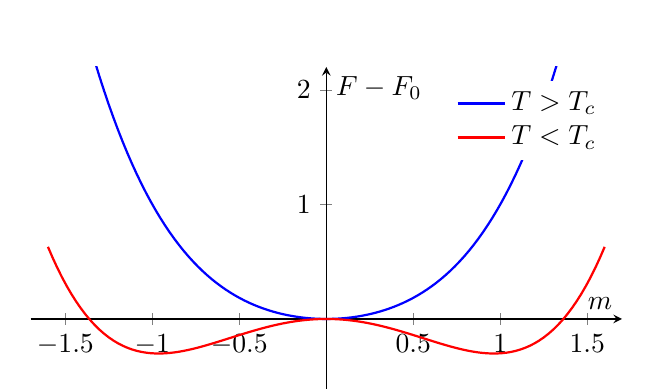
\begin{tikzpicture}
\begin{axis}[width=0.75\textwidth,height=5.8cm,
xlabel={$m$},ylabel={$F-F_0$},axis lines=middle,
xmin=-1.7,xmax=1.7,ymin=-0.7,ymax=2.2,samples=120,
legend style={draw=none,at={(0.98,0.96)},anchor=north east}]
\addplot[blue,thick,domain=-1.6:1.6] {0.65*x^2+0.35*x^4};
\addlegendentry{$T>T_c$}
\addplot[red,thick,domain=-1.6:1.6] {-0.65*x^2+0.35*x^4};
\addlegendentry{$T<T_c$}
\end{axis}
\end{tikzpicture}
\caption{Landau 自由能从单阱变为双阱，展示序参量的自发选择。}
\end{figure}

\begin{whybox}
为什么必须先确定序参量和对称性？Landau 展开允许的项由对称性决定。铁磁体零场下有 $m\to-m$，不能出现奇次项；若外场非零，$-hm$ 显式破坏该对称性。密度波序参量通常是复数，其相位对应平移；超导序参量也是复数，但还与电磁规范耦合。
\end{whybox}

\section{经典相变与量子相变}
经典连续相变由温度驱动，临界涨落主要是热涨落。量子相变发生在 $T=0$，由压力、磁场、掺杂或相互作用强度等非热参数调控，涨落来自不确定性。虚时间路径积分把 $d$ 维量子系统映射到额外含时间维的经典问题，动态临界指数 $z$ 描述
\[
\xi_\tau\sim\xi^z.
\]
有限温度会截断虚时间长度 $\hbar/\kb T$，在量子临界扇区产生非费米液体或非常规标度。面试中不必背所有指数，但要区分“零温基态重排”和普通热相变。

\section{线性响应与 Kubo 公式的物理结构}
若外扰
$H'(t)=-f(t)B$，一阶响应
\[
\delta\langle A(t)\rangle
=\int_{-\infty}^{t}\chi_{AB}(t-t')f(t')\dd t',
\]
\[
\boxed{\chi_{AB}(t)=\frac{i}{\hbar}\theta(t)
\langle[B(0),A(t)]\rangle_0}.
\]
$\theta(t)$ 保证因果性；对易子反映量子涨落。频域中响应的实部常描述色散，虚部描述吸收。电导率、磁化率、介电函数和散射谱都可以放入这一框架。静态涨落-响应关系是它在低频平衡极限的影子。

\section{三个完整例题}
\begin{examplebox}
\textbf{例 1：顺磁自旋的涨落。}对 $N$ 个独立 Ising 磁矩
$m_i=\pm\mu$，零场 $\langle M\rangle=0$，
$\langle M^2\rangle=N\mu^2$。涨落-响应给
\[
\chi=\beta\langle M^2\rangle/V
=\frac{n\mu^2}{\kb T},
\]
即 Curie 定律。平均场加入有效场反馈后变为 Curie-Weiss 形式。
\end{examplebox}

\begin{examplebox}
\textbf{例 2：一维经典 Ising 为何无有限温铁磁序？}产生一个畴壁代价有限能量
$\Delta E=2J$，但畴壁可放在约 $N$ 个位置，熵增
$\Delta S\simeq\kb\ln N$。任意 $T>0$ 下大系统的
$\Delta F=2J-\kb T\ln N$ 最终为负，畴壁增殖破坏长程有序。
\end{examplebox}

\begin{examplebox}
\textbf{例 3：由低温比热分离电子和声子。}若实验拟合
$C/T=\gamma+\beta T^2$，作 $C/T$ 对 $T^2$ 图，截距为 $\gamma$；由
\[
\beta=\frac{12\pi^4}{5}\frac{N\kb}{\Theta_D^3}
\]
可估算 $\Theta_D$。若低温出现指数衰减或跳变，则可能提示超导能隙或相变。
\end{examplebox}

\section{面试总结与自测}
\begin{interviewbox}
\textbf{配分函数为什么重要？}它是带权微观态计数，也是热力学量的生成函数；一阶导数给平均值，二阶导数给涨落和响应。回答时应给
$F=-\kb T\ln Z$、$U=-\partial_\beta\ln Z$ 与
$\langle(\Delta E)^2\rangle=\kb T^2C_V$ 三层关系。

\textbf{量子相变与经典相变有何不同？}先说驱动参数和涨落来源，再说有限温交叉和动态指数，不要把“发生在低温”当定义。
\end{interviewbox}
\begin{selftestbox}
\begin{enumerate}
\item 用最大熵法推导巨正则分布。
\item 推导能量涨落与热容关系，并估算相对涨落尺度。
\item 化学势在 Bose 与 Fermi 系统中的约束有何不同？
\item Sommerfeld 展开的适用条件是什么？
\item 为什么金属低温常画 $C/T$ 对 $T^2$？
\item 从 Landau 自由能求 $\beta_{\rm MF},\gamma_{\rm MF}$。
\item 梯度项如何定义关联长度？
\item 为什么一维短程 Ising 模型没有有限温相变？
\item Kubo 响应函数中的阶跃函数有何意义？
\item 声子、磁振子、电子分别服从什么统计，化学势如何处理？
\end{enumerate}
\end{selftestbox}


\part{电动力学}
\label{part:electrodynamics}
\renewcommand{\currentparttitle}{电动力学}
\chapter{电动力学概念骨架：场、波与规范}
\section{Maxwell 方程}
\[
\begin{array}{c|c}
\text{微分形式}&\text{积分形式}\\ \hline
\nabla\cdot\vb E=\rho/\varepsilon_0&\oint\vb E\cdot\dd\vb a=Q/\varepsilon_0\\
\nabla\cdot\vb B=0&\oint\vb B\cdot\dd\vb a=0\\
\nabla\times\vb E=-\partial_t\vb B&\oint\vb E\cdot\dd\vb l=-\dd\Phi_B/\dd t\\
\nabla\times\vb B=\mu_0\vb J+\mu_0\varepsilon_0\partial_t\vb E&
\oint\vb B\cdot\dd\vb l=\mu_0I+\mu_0\varepsilon_0\dd\Phi_E/\dd t
\end{array}
\]
四式依次表达电荷是电场源、无磁单极、变化磁场产生涡旋电场、传导电流与变化电场产生磁场。位移电流项还保证
$\partial_t\rho+\nabla\cdot\vb J=0$。

\section{静场、Green 函数与镜像法}
静电场 $\vb E=-\nabla\phi$，代入 Gauss 定律：
\[
\nabla^2\phi=-\rho/\varepsilon_0,
\]
无源区即 Laplace 方程。自由空间 Green 函数满足
$\nabla^2G(\vb r,\vb r')=-\delta(\vb r-\vb r')$，
$G=1/(4\pi|\vb r-\vb r'|)$，从而
$\phi=\varepsilon_0^{-1}\int G\rho\,\dd^3r'$ 加边界项。接地无限导体平面上方的点电荷，可在镜像位置放置 $-q$；上半空间边界条件相同，唯一性定理保证所得场正确，但镜像电荷不是真实源。

静磁场因 $\nabla\cdot\vb B=0$ 可写 $\vb B=\nabla\times\vb A$。取 Coulomb 规范
$\nabla\cdot\vb A=0$，由 $\nabla\times(\nabla\times\vb A)=\mu_0\vb J$ 得
\[
\nabla^2\vb A=-\mu_0\vb J.
\]

\section{电磁波、能流与规范}
真空无源区对 Faraday 定律取旋度：
\[
\nabla\times\nabla\times\vb E=\nabla(\nabla\cdot\vb E)-\nabla^2\vb E
=-\mu_0\varepsilon_0\partial_t^2\vb E,
\]
因 $\nabla\cdot\vb E=0$，
\[
\boxed{\nabla^2\vb E-\frac1{c^2}\partial_t^2\vb E=0},\qquad
c=(\mu_0\varepsilon_0)^{-1/2}.
\]
平面波代入散度方程得到 $\vb k\cdot\vb E=\vb k\cdot\vb B=0$，且
$\vb B=(1/\omega)\vb k\times\vb E$，所以真空波横向。偏振描述 $\vb E$ 端点轨迹；能流为
$\vb S=\vb E\times\vb H$。

势表示
\[
\vb B=\nabla\times\vb A,\qquad
\vb E=-\nabla\phi-\partial_t\vb A
\]
在变换
$\vb A'=\vb A+\nabla\chi,\ \phi'=\phi-\partial_t\chi$ 下不变。规范自由度是描述冗余而非新物理；选 Coulomb 或 Lorenz 规范是方便计算。四维记号中
$J^\mu=(c\rho,\vb J)$，$A^\mu=(\phi/c,\vb A)$，
$F^{\mu\nu}=\partial^\mu A^\nu-\partial^\nu A^\mu$；Maxwell 方程压缩为
$\partial_\mu F^{\mu\nu}=\mu_0J^\nu$ 和 Bianchi 恒等式。

\pitfall{电磁波横向结论这里限定真空均匀无源区；波导中可有纵向分量。规范势可变不表示势毫无意义，Aharonov--Bohm 效应体现其量子相位作用。}
\section{核心公式与面试回答}
\interview{推导波动方程时务必依次说“取旋度—用矢量恒等式—使用无源散度方程—代入另一条旋度方程”。回答规范不变性时直接代入势变换，展示二阶混合偏导抵消。}

\chapter{从作用量到传播与辐射}

\begin{prereqbox}
熟悉四维指标记号和分部积分。采用度规
$g_{\mu\nu}=\mathrm{diag}(1,-1,-1,-1)$，
$x^\mu=(ct,\vb r)$，
$A^\mu=(\phi/c,\vb A)$，
$J^\mu=(c\rho,\vb J)$。重复指标求和。不同教材的度规和势定义会改变若干符号，面试时应先声明约定。
\end{prereqbox}

\section{为什么从作用量出发}
Maxwell 方程若只作为四条经验公式记忆，规范自由度、守恒律和相对论结构彼此分离。作用量把它们统一：
\[
S[A]=\int\dd^4x\,\mathcal L,\qquad
\mathcal L=-\frac1{4\mu_0}F_{\mu\nu}F^{\mu\nu}-J_\mu A^\mu,
\]
\[
F_{\mu\nu}=\partial_\mu A_\nu-\partial_\nu A_\mu.
\]
第一项是自由场，第二项是外源与场的最小线性耦合。系数 $1/4$ 同时补偿
$F_{\mu\nu}$ 反对称导致的重复计数和变分时出现的因子 $2$。

\section{逐项变分推出非齐次 Maxwell 方程}
令 $A_\mu\to A_\mu+\delta A_\mu$，并要求变分在时空积分边界消失。首先
\[
\delta F_{\mu\nu}
=\partial_\mu\delta A_\nu-\partial_\nu\delta A_\mu.
\]
自由场项的变分是
\[
\delta S_f=-\frac1{4\mu_0}\int\dd^4x\,
\delta(F_{\mu\nu}F^{\mu\nu})
=-\frac1{2\mu_0}\int\dd^4x\,F^{\mu\nu}\delta F_{\mu\nu}.
\]
代入 $\delta F_{\mu\nu}$：
\[
\delta S_f=-\frac1{2\mu_0}\int\dd^4x\,
F^{\mu\nu}(\partial_\mu\delta A_\nu-\partial_\nu\delta A_\mu).
\]
第二项交换哑指标 $\mu\leftrightarrow\nu$，并用
$F^{\nu\mu}=-F^{\mu\nu}$：
\[
-F^{\mu\nu}\partial_\nu\delta A_\mu
=+F^{\nu\mu}\partial_\mu\delta A_\nu
=-F^{\mu\nu}\partial_\mu\delta A_\nu.
\]
因此两项相同，
\[
\delta S_f=-\frac1{\mu_0}\int\dd^4x\,
F^{\mu\nu}\partial_\mu\delta A_\nu.
\]
对 $\partial_\mu$ 分部积分：
\[
\delta S_f=
-\frac1{\mu_0}\int_{\partial\Omega}\dd\Sigma_\mu
F^{\mu\nu}\delta A_\nu
+\frac1{\mu_0}\int_\Omega\dd^4x\,
(\partial_\mu F^{\mu\nu})\delta A_\nu.
\]
边界变分为零，第一项消失。源项给
\[
\delta S_J=-\int\dd^4x\,J^\nu\delta A_\nu.
\]
合并：
\[
\delta S=\int\dd^4x\left[
\frac1{\mu_0}\partial_\mu F^{\mu\nu}-J^\nu
\right]\delta A_\nu.
\]
由于内部任意 $\delta A_\nu$ 都应使 $\delta S=0$，得到
\[
\boxed{\partial_\mu F^{\mu\nu}=\mu_0J^\nu}.
\]

\subsection{拆回三维形式}
取 $\nu=0$，利用
$F^{i0}=E_i/c$ 与 $\partial_i=\partial/\partial x_i$：
\[
\partial_iF^{i0}=\frac1c\nabla\cdot\vb E
=\mu_0c\rho,
\]
即
\[
\nabla\cdot\vb E=\mu_0c^2\rho=\rho/\varepsilon_0.
\]
取 $\nu=i$，时间项和空间项分别产生位移电流与磁场旋度，得到
\[
\nabla\times\vb B-\frac1{c^2}\pdv{\vb E}{t}
=\mu_0\vb J.
\]
这正是 Gauss 电定律和 Ampère--Maxwell 定律。

\section{齐次方程不是新的运动方程}
因为 $F=\dd A$，恒有
\[
\partial_\lambda F_{\mu\nu}
+\partial_\mu F_{\nu\lambda}
+\partial_\nu F_{\lambda\mu}=0.
\]
把 $F_{\mu\nu}=\partial_\mu A_\nu-\partial_\nu A_\mu$ 展开，所有二阶混合偏导两两抵消。这是 Bianchi 恒等式，不依赖作用量极值。其三维内容为
\[
\boxed{\nabla\cdot\vb B=0,\qquad
\nabla\times\vb E=-\pdv{\vb B}{t}}.
\]
因此四条 Maxwell 方程中，两条是作用量给出的动力学方程，两条来自用势表示场的几何恒等式。

\section{规范不变性与电荷守恒}
规范变换
\[
A_\mu\to A_\mu+\partial_\mu\chi
\]
不改变 $F_{\mu\nu}$。源耦合的变化为
\[
\delta_\chi S_J=-\int\dd^4x\,J^\mu\partial_\mu\chi.
\]
分部积分：
\[
\delta_\chi S_J
=-\int_{\partial\Omega}\dd\Sigma_\mu J^\mu\chi
+\int_\Omega\dd^4x\,\chi\,\partial_\mu J^\mu.
\]
边界项消失时，作用量对任意 $\chi$ 规范不变要求
\[
\boxed{\partial_\mu J^\mu=0}
\quad\Longleftrightarrow\quad
\pdv\rho t+\nabla\cdot\vb J=0.
\]
反过来，对场方程取 $\partial_\nu$：
\[
\partial_\nu\partial_\mu F^{\mu\nu}
=\mu_0\partial_\nu J^\nu.
\]
左边因偏导对称、$F$ 反对称而为零，也推出连续性方程。

\begin{pitfallbox}
规范变换是同一物理场的冗余描述，不是把一种物理状态变成另一种。所谓“规范对称性自发破缺”在严格表述中需要谨慎；超导中真正可观测的是规范不变相位梯度、磁通量子和相位刚度。
\end{pitfallbox}

\section{Lorenz 规范与波动方程}
将 $F^{\mu\nu}$ 展开：
\[
\partial_\mu F^{\mu\nu}
=\partial_\mu\partial^\mu A^\nu
-\partial^\nu(\partial_\mu A^\mu).
\]
定义 d'Alembert 算符
\[
\Box=\partial_\mu\partial^\mu
=\frac1{c^2}\frac{\partial^2}{\partial t^2}-\nabla^2.
\]
选择 Lorenz 规范
\[
\partial_\mu A^\mu=0
\quad\Longleftrightarrow\quad
\nabla\cdot\vb A+\frac1{c^2}\pdv\phi t=0,
\]
场方程化为四个波动方程
\[
\boxed{\Box A^\nu=\mu_0J^\nu}.
\]
规范并未完全固定：若 $\Box\chi=0$，则
$A_\mu+\partial_\mu\chi$ 仍满足 Lorenz 规范，这称剩余规范自由度。

\section{波动方程的推迟 Green 函数}
要求 Green 函数满足
\[
\Box G(x-x')=\delta^{(4)}(x-x').
\]
解可写为
\[
A^\mu(x)=\mu_0\int\dd^4x'\,G(x-x')J^\mu(x').
\]
物理上要求原因先于结果，即 $G(t<t')=0$，选择推迟 Green 函数。三维形式为
\[
G_{\rm ret}(\vb r,t;\vb r',t')
=\frac{\delta(t-t'-R/c)}{4\pi R},
\qquad R=|\vb r-\vb r'|.
\]
把它代回并先做 $t'$ 积分：
\[
\boxed{
\phi(\vb r,t)=\frac1{4\pi\varepsilon_0}
\int\frac{\rho(\vb r',t-R/c)}R\,\dd^3r'},
\]
\[
\boxed{
\vb A(\vb r,t)=\frac{\mu_0}{4\pi}
\int\frac{\vb J(\vb r',t-R/c)}R\,\dd^3r'}.
\]
源必须在推迟时刻 $t_r=t-R/c$ 取值。传播速度 $c$ 并非事后加入，而是双曲型场方程和因果边界条件的结果。

\subsection{验证 Green 函数结构}
Fourier 变换到 $(\vb k,\omega)$：
\[
G(\vb k,\omega)
=\frac1{k^2-(\omega/c)^2}.
\]
极点怎样绕过实轴决定边界条件。推迟解对应把极点移到保证
$t<t'$ 时积分闭合后为零的一侧。静态极限 $\omega=0$ 给
$G(\vb k)=1/k^2$，反变换就是 $1/4\pi R$ 的 Coulomb Green 函数。

\section{静电多极展开}
局域电荷分布外部 $r\gg r'$：
\[
\frac1{|\vb r-\vb r'|}
=\frac1r+\frac{\vb r\cdot\vb r'}{r^3}
+\frac{3(\vb r\cdot\vb r')^2-r^2r'^2}{2r^5}
+\cdots.
\]
代入
$\phi=(4\pi\varepsilon_0)^{-1}\int\rho(\vb r')/|\vb r-\vb r'|\dd^3r'$。
定义
\[
Q=\int\rho\,\dd^3r',\qquad
\vb p=\int\vb r'\rho\,\dd^3r',
\]
\[
Q_{ij}=\int\rho(3x_i'x_j'-r'^2\delta_{ij})\dd^3r'.
\]
于是
\[
\phi(\vb r)=\frac1{4\pi\varepsilon_0}
\left[\frac Qr+\frac{\vb p\cdot\hat{\vb r}}{r^2}
+\frac1{2r^3}Q_{ij}\hat r_i\hat r_j+\cdots\right].
\]
若总电荷 $Q\ne0$，偶极矩依赖原点；若 $Q=0$，平移原点不改变 $\vb p$。远场最低非零多极矩支配势。

\section{唯一性定理与镜像法}
若两组势 $\phi_1,\phi_2$ 在区域内满足同一 Poisson 方程并具有相同 Dirichlet 边界值，差
$u=\phi_1-\phi_2$ 满足 $\nabla^2u=0$ 且边界 $u=0$。利用 Green 第一恒等式：
\[
\int_V|\nabla u|^2\dd V
=\oint_{\partial V}u\pdv u n\dd a-\int_Vu\nabla^2u\dd V=0.
\]
所以 $\nabla u=0$，$u$ 为常数；边界令常数为零。镜像法只需在物理区域内满足 Poisson 方程和导体边界条件，唯一性定理便保证解正确。

\section{Poynting 定理逐步推导}
从 Ampère--Maxwell 方程点乘 $\vb E$：
\[
\vb E\cdot(\nabla\times\vb H)
=\vb J\cdot\vb E+\vb E\cdot\pdv{\vb D}{t}.
\]
从 Faraday 方程点乘 $\vb H$：
\[
\vb H\cdot(\nabla\times\vb E)
=-\vb H\cdot\pdv{\vb B}{t}.
\]
用恒等式
\[
\nabla\cdot(\vb E\times\vb H)
=\vb H\cdot\nabla\times\vb E
-\vb E\cdot\nabla\times\vb H
\]
相减，在线性无色散介质中
\[
\vb E\cdot\pdv{\vb D}{t}
=\pdv{}{t}\left(\frac12\vb E\cdot\vb D\right),
\]
\[
\vb H\cdot\pdv{\vb B}{t}
=\pdv{}{t}\left(\frac12\vb B\cdot\vb H\right).
\]
得到
\[
\boxed{\pdv u t+\nabla\cdot\vb S=-\vb J\cdot\vb E},
\]
\[
u=\frac12(\vb E\cdot\vb D+\vb B\cdot\vb H),
\qquad \vb S=\vb E\times\vb H.
\]
体积分形式表明：区域内场能变化 $+$ 流出表面的能流 $=$ 场对物质做功的负值。

\section{平面波、介质与 Fresnel 系数}
无源均匀介质取
$\vb E=\vb E_0e^{i(\vb k\cdot\vb r-\omega t)}$。
Maxwell 方程给
\[
\vb k\cdot\vb E_0=0,\qquad
\vb B_0=\frac1\omega\vb k\times\vb E_0,
\]
\[
k^2=\mu\varepsilon\omega^2,\qquad
v=\frac1{\sqrt{\mu\varepsilon}}.
\]
法向入射界面，切向 $E,H$ 连续。设入射、反射、透射振幅
$E_i,E_r,E_t$，波阻抗 $Z=\sqrt{\mu/\varepsilon}$：
\[
E_i+E_r=E_t,\qquad
\frac{E_i-E_r}{Z_1}=\frac{E_t}{Z_2}.
\]
解得
\[
r=\frac{E_r}{E_i}=\frac{Z_2-Z_1}{Z_2+Z_1},
\qquad
t=\frac{E_t}{E_i}=\frac{2Z_2}{Z_1+Z_2}.
\]
功率反射率 $R=|r|^2$；无耗散时需用 Poynting 流验证
$R+T=1$，其中 $T$ 含阻抗比。

\section{矩形波导的截止频率}
理想导体内切向电场为零。设波导横截面 $0<x<a,0<y<b$，沿
$z$ 传播。对 TM 模，纵向电场满足
\[
(\partial_x^2+\partial_y^2+k_c^2)E_z=0,
\quad E_z|_{\partial A}=0.
\]
分离变量得到
\[
E_z=E_0\sin\frac{m\pi x}{a}
\sin\frac{n\pi y}{b},
\]
\[
k_c^2=\left(\frac{m\pi}{a}\right)^2+
\left(\frac{n\pi}{b}\right)^2.
\]
纵向传播常数
\[
\beta^2=\frac{\omega^2}{c^2}-k_c^2.
\]
当 $\omega<ck_c$，$\beta$ 为虚数，模式指数衰减；截止频率
\[
\omega_c=ck_c.
\]
波导中场一般含纵向分量，因此“电磁波必为横波”只对均匀无界介质平面波成立。

\section{局域源的远区展开}
对尺寸 $d$ 的源，观察点 $r\gg d$：
\[
R=|\vb r-\vb r'|\simeq r-\hat{\vb r}\cdot\vb r',
\qquad
\frac1R\simeq\frac1r.
\]
推迟时间
\[
t-\frac Rc\simeq t-\frac rc+
\frac{\hat{\vb r}\cdot\vb r'}c.
\]
若源还满足长波条件 $d\ll\lambda$，最后一项相位可作展开。最低阶有时间变化的电偶极矩
\[
\vb p(t)=\int\vb r'\rho(\vb r',t)\dd^3r'.
\]
利用连续性方程：
\[
\dot{\vb p}
=\int\vb r'\pdv\rho t\dd^3r'
=-\int\vb r'\nabla'\cdot\vb J\,\dd^3r'.
\]
分部积分且局域源边界项消失：
\[
\boxed{\dot{\vb p}=\int\vb J\,\dd^3r'}.
\]
因此远区矢势最低阶为
\[
\vb A(\vb r,t)\simeq
\frac{\mu_0}{4\pi r}\dot{\vb p}(t-r/c).
\]

\section{电偶极辐射}
远区只保留 $1/r$ 项。由
$\vb B=\nabla\times\vb A$，对推迟时间求空间导数产生
$-\,\hat{\vb r}\partial_t/c$：
\[
\boxed{\vb B_{\rm rad}
=\frac{\mu_0}{4\pi cr}
\ddot{\vb p}(t-r/c)\times\hat{\vb r}}.
\]
远区局部像平面波，
\[
\boxed{\vb E_{\rm rad}
=c\,\vb B_{\rm rad}\times\hat{\vb r}
=\frac1{4\pi\varepsilon_0c^2r}
\hat{\vb r}\times(\ddot{\vb p}\times\hat{\vb r})}.
\]
若 $\vb p=p_0\cos\omega t\,\hat{\vb z}$，
\[
E_\theta=\frac{p_0\omega^2}{4\pi\varepsilon_0c^2r}
\sin\theta\cos[\omega(t-r/c)].
\]
周期平均 Poynting 流
\[
\avg S_r=\frac{p_0^2\omega^4}{32\pi^2
\varepsilon_0c^3r^2}\sin^2\theta.
\]
每立体角功率
\[
\boxed{\dv{\avg P}{\Omega}
=\frac{p_0^2\omega^4}{32\pi^2\varepsilon_0c^3}
\sin^2\theta}.
\]
积分
$\int\sin^2\theta\,\dd\Omega=8\pi/3$：
\[
\boxed{\avg P
=\frac{p_0^2\omega^4}{12\pi\varepsilon_0c^3}}.
\]
辐射沿偶极轴为零、赤道最大，且有强烈的 $\omega^4$ 依赖。

\section{近区、感应区和辐射区}
振荡偶极完整场包含
\[
E\sim\frac p{r^3}
+\frac{\dot p}{cr^2}
+\frac{\ddot p}{c^2r}.
\]
$1/r^3$ 是准静电近场，$1/r^2$ 是感应场，$1/r$ 是辐射场。只有辐射项使
$r^2S_r$ 在 $r\to\infty$ 保持有限总功率。近场能量在源和场之间往返交换，不代表净辐射。

\section{点电荷、Liénard--Wiechert 势与 Larmor 公式}
点电荷轨迹 $\vb r_q(t)$ 的源为
\[
\rho(\vb r,t)=q\delta[\vb r-\vb r_q(t)],
\qquad
\vb J=\rho\,\vb v(t).
\]
代入推迟势时，$\delta$ 函数的变量也依赖推迟时刻，积分产生 Jacobian
$\kappa=1-\hat{\vb n}\cdot\vb\beta$。得到
\[
\phi(\vb r,t)=
\left.\frac{q}{4\pi\varepsilon_0}
\frac1{\kappa R}\right|_{\rm ret},
\qquad
\vb A=\left.\frac{\vb v}{c^2}\phi\right|_{\rm ret}.
\]
求导后电场分成速度场与加速度场：
\[
\vb E=
\frac{q}{4\pi\varepsilon_0}
\left[
\frac{(1-\beta^2)(\hat{\vb n}-\vb\beta)}
{\kappa^3R^2}
+\frac{\hat{\vb n}\times[
(\hat{\vb n}-\vb\beta)\times\dot{\vb\beta}]}
c{\kappa^3R}
\right]_{\rm ret}.
\]
第一项 $\sim1/R^2$，第二项 $\sim1/R$ 并负责辐射。非相对论极限
$\beta\ll1$：
\[
\vb E_{\rm rad}
=\frac{q}{4\pi\varepsilon_0c^2R}
\hat{\vb n}\times(\hat{\vb n}\times\vb a).
\]
角积分得到 Larmor 功率
\[
\boxed{P=\frac{q^2a^2}{6\pi\varepsilon_0c^3}}.
\]
它与偶极辐射一致：单电荷偶极矩 $\vb p=q\vb r_q$，故
$\ddot{\vb p}=q\vb a$。

\section{完整例题：短偶极天线}
长度 $\ell\ll\lambda$ 的细导线电流近似
$I(t)=I_0\cos\omega t$。端点电荷满足
$\dot q=I$，偶极矩幅值
\[
p_0=q_0\ell=\frac{I_0\ell}{\omega}.
\]
代入偶极总辐射功率：
\[
\avg P=\frac{I_0^2\ell^2\omega^2}
{12\pi\varepsilon_0c^3}.
\]
若用峰值电流定义辐射电阻
$\avg P=I_0^2R_{\rm rad}/2$，则
\[
R_{\rm rad}=\frac{\ell^2\omega^2}
{6\pi\varepsilon_0c^3}
=80\pi^2\left(\frac{\ell}{\lambda}\right)^2\Omega.
\]
这展示了场论推导如何转化为可测的电路参数。

\section{面试表达与自测}
\begin{interviewbox}
\textbf{30 秒：}自由电磁场作用量由唯一的最低阶 Lorentz 标量
$F_{\mu\nu}F^{\mu\nu}$ 构成。对势变分给非齐次 Maxwell 方程；
$F=\dd A$ 自动给齐次方程；规范不变性要求电流守恒。Lorenz 规范把势化成波动方程，推迟 Green 函数保证因果传播，远区展开再给偶极辐射。

\textbf{黑板版：}至少能完整写出
$\delta(F^2)$、利用反对称性合并两项、分部积分、消去边界项和得到
$\partial_\mu F^{\mu\nu}=\mu_0J^\nu$ 的五步。
\end{interviewbox}
\begin{selftestbox}
\begin{enumerate}
\item 为什么场作用量系数是 $-1/4\mu_0$？
\item 变分时反对称性怎样把两项合并？
\item 齐次 Maxwell 方程为何是恒等式？
\item 规范不变性和电荷守恒的逻辑关系是什么？
\item 推迟与超前 Green 函数满足同一微分方程，物理上如何选择？
\item 多极展开的适用条件是什么？
\item 唯一性定理怎样保证镜像法？
\item 从哪一个矢量恒等式推出 Poynting 定理？
\item Fresnel 功率透射率为什么不总等于 $|t|^2$？
\item 波导截止的数学来源是什么？
\item 偶极远场中为什么出现 $\ddot p$？
\item 如何按 $1/r$ 幂次区分近场和辐射场？
\item Liénard--Wiechert 势中的 $\kappa$ 从哪里来？
\item Larmor 公式与偶极辐射如何相互验证？
\end{enumerate}
\end{selftestbox}

\chapter{波导模式与相对论电动力学}

\begin{mapbox}
第一部分仍使用 SI 制，从频域 Maxwell 方程推导 TE、TM、TEM 的纵向本征问题和横向场。第二部分改用 Gaussian 几何单位制并令 $c=1$，以作用量、场张量和 Lorentz 变换呈现相对论结构。两种单位制不在同一推导中混用。
\end{mapbox}

\section{频域 Maxwell 方程与纵横分解（SI）}
均匀、无源、无耗介质中取时间依赖 $e^{-i\omega t}$：
\[
\nabla\times\vb E=i\omega\mu\vb H,\qquad
\nabla\times\vb H=-i\omega\varepsilon\vb E,
\]
\[
\nabla\cdot\vb E=\nabla\cdot\vb H=0.
\]
沿 $z$ 传播的模式写成 $e^{i\beta z}$。分解
\[
\vb E=\vb E_t+\hat{\vb z}E_z,\qquad
\nabla=\nabla_t+i\beta\hat{\vb z}.
\]
定义介质波数 $k=\omega\sqrt{\mu\varepsilon}$ 和
\[
k_c^2=k^2-\beta^2.
\]
把 Maxwell 方程的纵向、横向分量联立消元，可得
\[
\boxed{
\vb E_t=\frac{i}{k_c^2}
\left[\beta\nabla_tE_z
+\omega\mu\,\hat{\vb z}\times\nabla_tH_z\right]},
\]
\[
\boxed{
\vb H_t=\frac{i}{k_c^2}
\left[\beta\nabla_tH_z
-\omega\varepsilon\,\hat{\vb z}\times\nabla_tE_z\right]}.
\]
同时纵向分量都满足二维 Helmholtz 方程：
\[
(\nabla_t^2+k_c^2)E_z=0,\qquad
(\nabla_t^2+k_c^2)H_z=0.
\]
因此只要解出 $E_z$ 或 $H_z$，其余四个横向分量就由上式唯一确定。

\section{TM、TE 与 TEM 的定义}
\[
\begin{array}{c|cc}
&E_z&H_z\\ \hline
\mathrm{TM}&\ne0&0\\
\mathrm{TE}&0&\ne0\\
\mathrm{TEM}&0&0
\end{array}
\]
TM 表示磁场完全横向；TE 表示电场完全横向。波导模式一般并非
$\vb E,\vb H$ 都横向。

理想导体边界上 $\vb E_{\parallel}=0$。对 TM 模，$E_z$ 沿导体壁切向，故
\[
E_z|_{\partial A}=0
\]
是 Dirichlet 条件。对 TE 模，将 $\vb E_t$ 公式投影到壁面切向，可得
\[
\pdv{H_z}{n}\bigg|_{\partial A}=0,
\]
即 Neumann 条件。

\section{矩形波导的 TM 模}
横截面 $0<x<a,\ 0<y<b$。分离变量
$E_z=X(x)Y(y)$：
\[
\frac{X''}{X}+\frac{Y''}{Y}=-k_c^2.
\]
四条边 $E_z=0$，故
\[
E_z=E_0\sin\frac{m\pi x}{a}\sin\frac{n\pi y}{b},
\]
\[
k_c^2=\left(\frac{m\pi}{a}\right)^2+
\left(\frac{n\pi}{b}\right)^2,\qquad m,n=1,2,\ldots.
\]
若任一指标为零，$E_z$ 恒为零，所以不存在 TM$_{m0}$ 或 TM$_{0n}$。
由纵横关系得到
\[
E_x=\frac{i\beta}{k_c^2}\pdv{E_z}{x},\quad
E_y=\frac{i\beta}{k_c^2}\pdv{E_z}{y},
\]
\[
H_x=\frac{i\omega\varepsilon}{k_c^2}\pdv{E_z}{y},\quad
H_y=-\frac{i\omega\varepsilon}{k_c^2}\pdv{E_z}{x}.
\]

\section{矩形波导的 TE 模}
Neumann 条件允许余弦解：
\[
H_z=H_0\cos\frac{m\pi x}{a}\cos\frac{n\pi y}{b},
\]
\[
k_c^2=\left(\frac{m\pi}{a}\right)^2+
\left(\frac{n\pi}{b}\right)^2,
\]
其中 $m,n$ 可以有一个为零，但不能同时为零。横向场为
\[
H_x=\frac{i\beta}{k_c^2}\pdv{H_z}{x},\quad
H_y=\frac{i\beta}{k_c^2}\pdv{H_z}{y},
\]
\[
E_x=-\frac{i\omega\mu}{k_c^2}\pdv{H_z}{y},\quad
E_y=\frac{i\omega\mu}{k_c^2}\pdv{H_z}{x}.
\]
若 $a>b$，最低截止波数是 $k_c=\pi/a$，主模为 TE$_{10}$：
\[
H_z=H_0\cos\frac{\pi x}{a},\qquad
\omega_c=\frac{\pi}{a\sqrt{\mu\varepsilon}}.
\]

\section{截止、色散、速度与波阻抗}
\[
\boxed{\beta^2=k^2-k_c^2
=\mu\varepsilon(\omega^2-\omega_c^2)}.
\]
$\omega>\omega_c$ 时 $\beta$ 为实数，模式传播；低于截止时场沿 $z$ 指数衰减。相速度与群速度
\[
v_p=\frac{\omega}{\beta}
=\frac{v}{\sqrt{1-(\omega_c/\omega)^2}},
\]
\[
v_g=\pdv\omega\beta
=v\sqrt{1-(\omega_c/\omega)^2},
\qquad v=\frac1{\sqrt{\mu\varepsilon}},
\]
所以
\[
\boxed{v_pv_g=v^2}.
\]
$v_p>v$ 不传递信息；包络和能量以 $v_g<v$ 传播。横向场幅度比定义模式阻抗：
\[
Z_{\rm TE}=\frac{\omega\mu}{\beta}
=\frac{Z}{\sqrt{1-(\omega_c/\omega)^2}},
\]
\[
Z_{\rm TM}=\frac{\beta}{\omega\varepsilon}
=Z\sqrt{1-(\omega_c/\omega)^2},
\quad Z=\sqrt{\mu/\varepsilon}.
\]

\section{TEM 模为何需要多连通截面}
若 $E_z=H_z=0$ 且 $k_c=0$，横向场满足二维静电问题
\[
\nabla_t\times\vb E_t=0,\qquad
\nabla_t\cdot\vb E_t=0.
\]
可写 $\vb E_t=-\nabla_t\phi$，其中 $\nabla_t^2\phi=0$。单一空心金属管的整个边界为同一等势面，唯一性定理迫使 $\phi$ 为常数，故不存在非零 TEM 模。同轴线有内外两个独立导体，可以维持电势差，因此支持 TEM。其
\[
\beta=k,\quad v_p=v_g=v,\quad Z_{\rm TEM}=Z
\]
且无截止频率。

\section{模式正交、功率与谐振腔}
二维 Helmholtz 算符在相应边界条件下自伴，不同 $k_c^2$ 的本征函数正交。时间平均功率
\[
P=\frac12\operatorname{Re}\int_A
(\vb E\times\vb H^*)\cdot\hat{\vb z}\,\dd A.
\]
正交性使不同模式的交叉功率积分为零。若在 $z$ 方向再以 PEC 封闭成长度 $d$ 的矩形腔，纵向驻波要求
$k_z=p\pi/d$，谐振频率
\[
\boxed{
\omega_{mnp}=\frac1{\sqrt{\mu\varepsilon}}
\sqrt{\left(\frac{m\pi}{a}\right)^2+
\left(\frac{n\pi}{b}\right)^2+
\left(\frac{p\pi}{d}\right)^2}}.
\]
品质因数 $Q=\omega U/P_{\rm loss}$ 衡量每周期损耗相对储能。

\begin{examplebox}[title=TE$_{10}$ 的截止与色散]
空气波导 $a=2.0\,\mathrm{cm}$。主模截止频率
\[
f_c=\frac{c}{2a}=7.5\,\mathrm{GHz}.
\]
若工作频率 $f=10\,\mathrm{GHz}$，
\[
v_g=c\sqrt{1-(f_c/f)^2}\simeq0.661c,
\quad
v_p=\frac{c^2}{v_g}\simeq1.51c.
\]
乘积仍为 $c^2$，所以超光速相速度没有违反相对论。
\end{examplebox}

\chapter{高斯几何单位制相对论电动力学（光速归一为 1）}

\begin{prereqbox}
本章约定度规 $g_{\mu\nu}=\operatorname{diag}(1,-1,-1,-1)$，
$x^\mu=(t,\vb r)$，并设 $c=1$。时间与长度具有相同量纲，速度是以真空光速为单位的无量纲量，故
$\gamma=(1-v^2)^{-1/2}$。以下公式均为 Gaussian 几何单位制；电荷和场的量纲与 SI 不同。恢复 $c$ 时必须依据量纲和四维定义统一恢复，不能只在个别公式中补写 $c$。
\end{prereqbox}

\section{SI 与 Gaussian 几何制的必要对照}
\[
\begin{array}{c|c|c}
&\mathrm{SI}&\mathrm{Gaussian},\ c=1\\ \hline
\nabla\cdot\vb E&\rho/\varepsilon_0&4\pi\rho\\
\nabla\times\vb B&\mu_0\vb J+c^{-2}\partial_t\vb E&
\ 4\pi\vb J+\partial_t\vb E\\
\nabla\times\vb E&-\partial_t\vb B&-\partial_t\vb B\\
\vb F/q&\vb E+\vb v\times\vb B&
\vb E+\vb v\times\vb B\\
u&(\varepsilon_0E^2+B^2/\mu_0)/2&(E^2+B^2)/(8\pi)
\end{array}
\]
Gaussian 制中 $\vb E,\vb B$ 具有相同量纲；再令 $c=1$ 后，光锥为
$t^2-r^2=0$，四维公式中不再出现人为的 $c$ 因子。表中两列的数值不可直接相等，它们只是同一物理定律在不同单位约定下的形式对照。
本章的三维 Maxwell 方程统一写为
\[
\nabla\cdot\vb E=4\pi\rho,\qquad
\nabla\cdot\vb B=0,
\]
\[
\nabla\times\vb E=-\partial_t\vb B,\qquad
\nabla\times\vb B=4\pi\vb J+\partial_t\vb E.
\]

\section{粒子作用量推出 Lorentz 力}
在 $c=1$ 的 Gaussian 几何单位中，带电粒子的作用量为
\[
\boxed{S_p=-m\int\dd s-q\int A_\mu\dd x^\mu}.
\]
用坐标时间 $t$ 参数化，且取
$A_\mu\dd x^\mu=\phi\,\dd t-\vb A\cdot\dd\vb r$：
\[
L=-m\sqrt{1-v^2}+q\vb A\cdot\vb v-q\phi.
\]
正则动量
\[
\pdv L{\vb v}=\gamma m\vb v+q\vb A.
\]
Euler--Lagrange 方程的第 $i$ 分量：
\[
\dv{}{t}\left(\gamma mv_i+qA_i\right)
=qv_j\partial_iA_j-q\partial_i\phi.
\]
移项并使用
\[
v_j(\partial_iA_j-\partial_jA_i)
=[\vb v\times(\nabla\times\vb A)]_i
\]
以及
$\vb E=-\nabla\phi-\partial_t\vb A$，得到
\[
\boxed{\dv{}t(\gamma m\vb v)
=q\left(\vb E+\vb v\times\vb B\right)}.
\]
$v<1$ 对应有质量粒子低于光速。若恢复普通单位，$\vb v$ 换成
$\vb v/c$，右侧磁力项恢复为 $q\vb v\times\vb B/c$。

\section{场作用量与协变 Maxwell 方程}
定义
\[
A^\mu=(\phi,\vb A),\qquad A_\mu=(\phi,-\vb A),
\]
\[
J^\mu=(\rho,\vb J),\qquad J_\mu=(\rho,-\vb J).
\]
取
\[
S[A]=-\frac1{16\pi}\int F_{\mu\nu}F^{\mu\nu}\dd^4x
-\int J_\mu A^\mu\dd^4x,
\]
\[
F_{\mu\nu}=\partial_\mu A_\nu-\partial_\nu A_\mu.
\]
变分
\[
\delta(F_{\mu\nu}F^{\mu\nu})
=2F^{\mu\nu}(\partial_\mu\delta A_\nu-\partial_\nu\delta A_\mu)
=4F^{\mu\nu}\partial_\mu\delta A_\nu,
\]
其中最后一步使用 $F^{\mu\nu}=-F^{\nu\mu}$。分部积分：
\[
\delta S=
\frac1{4\pi}\int(\partial_\mu F^{\mu\nu})\delta A_\nu\dd^4x
-\int J^\nu\delta A_\nu\dd^4x,
\]
边界项因 $\delta A_\nu|_{\partial\mathcal M}=0$ 消失。任意变分给
\[
\boxed{\partial_\mu F^{\mu\nu}=4\pi J^\nu}.
\]
另一方面 $F=\dd A$ 自动满足
\[
\boxed{\partial_\lambda F_{\mu\nu}
+\partial_\mu F_{\nu\lambda}
+\partial_\nu F_{\lambda\mu}=0}.
\]
二者分别对应非齐次和齐次 Maxwell 方程。

\section{规范不变性与连续性方程}
\[
A_\mu\to A_\mu+\partial_\mu\chi
\]
不改变 $F_{\mu\nu}$。源耦合项变化
\[
\delta S_{\rm int}
=-\int J^\mu\partial_\mu\chi\,\dd^4x
=\int(\partial_\mu J^\mu)\chi\,\dd^4x
\]
（舍去边界项）。要对任意 $\chi$ 保持规范不变，必须
\[
\boxed{\partial_\mu J^\mu=0}
\quad\Longleftrightarrow\quad
\partial_t\rho+\nabla\cdot\vb J=0.
\]
也可直接对场方程取 $\partial_\nu$，因对称导数收缩反对称张量恒为零而得到同一结论。

\section{场张量、Lorentz 变换与不变量}
一种一致约定为
\[
F^{\mu\nu}=
\begin{pmatrix}
0&-E_x&-E_y&-E_z\\
E_x&0&-B_z&B_y\\
E_y&B_z&0&-B_x\\
E_z&-B_y&B_x&0
\end{pmatrix}.
\]
沿 $x$ 方向速度 $\vb v=v\hat{\vb x}$ 的 boost 给
\[
E_x'=E_x,\quad B_x'=B_x,
\]
\[
\vb E_\perp'=\gamma(\vb E_\perp+\vb\beta\times\vb B),
\]
\[
\vb B_\perp'=\gamma(\vb B_\perp-\vb\beta\times\vb E),
\qquad \vb\beta=\vb v,\quad \gamma=(1-v^2)^{-1/2}.
\]
由张量收缩得到两个 Lorentz 不变量：
\[
\boxed{I_1=E^2-B^2},\qquad
\boxed{I_2=\vb E\cdot\vb B}.
\]
若 $I_2=0$ 且 $I_1>0$，存在某参考系使 $\vb B'=0$；若
$I_2=0$ 且 $I_1<0$，存在某系使 $\vb E'=0$。平面真空电磁波满足
$I_1=I_2=0$，不能通过有限 boost 变成纯电场或纯磁场。

\section{能动张量与局域守恒}
Gaussian 几何制电磁能动张量可写为
\[
T^{\mu\nu}=\frac1{4\pi}
\left(-F^{\mu\lambda}F^\nu{}_\lambda
+\frac14g^{\mu\nu}F_{\alpha\beta}F^{\alpha\beta}\right)
\]
（整体号随度规和 $F$ 定义而变，但物理分量固定）。其分量包含
\[
T^{00}=\frac{E^2+B^2}{8\pi},\qquad
T^{0i}=S_i,\qquad
\vb S=\frac1{4\pi}\vb E\times\vb B.
\]
利用 Maxwell 方程和 Bianchi 恒等式可得
\[
\boxed{\partial_\mu T^{\mu\nu}
=-F^{\nu\lambda}J_\lambda}.
\]
右侧是场对物质四维力密度的负值；把物质能动张量加入后，总能量动量局域守恒。

\begin{interviewbox}
\textbf{TE/TM 的回答顺序：}先按纵向分量定义，再说 $E_z,H_z$ 满足横向 Helmholtz 方程；PEC 使 TM 对应 Dirichlet、TE 对应 Neumann；本征值给截止频率，横向场由 Maxwell 方程恢复。TEM 要求 $k_c=0$，单连通空心金属管因唯一性定理不能支持它。

\textbf{相对论电动力学的回答顺序：}四维势生成反对称场张量；场作用量变分给非齐次 Maxwell 方程，$F=\dd A$ 给齐次方程；规范不变性要求电流守恒；$F^{\mu\nu}$ 的 Lorentz 变换统一解释电场和磁场的混合。
\end{interviewbox}

\begin{selftestbox}
\begin{enumerate}
\item 从频域 Maxwell 方程重新推出 $\vb E_t,\vb H_t$。
\item 为什么 TM 模的两个指标都不能为零？
\item 推导 TE 和 TM 模式阻抗。
\item 为什么 TE$_{10}$ 是 $a>b$ 矩形波导的主模？
\item 用唯一性定理说明空心矩形波导没有 TEM。
\item 从粒子作用量逐分量推出 $c=1$ 的 Gaussian 几何制 Lorentz 力。
\item 场作用量中的 $1/16\pi$ 为什么在变分后变成 $1/4\pi$？
\item 用两个场不变量判断能否找到纯电场参考系。
\end{enumerate}
\end{selftestbox}


\part{固体物理}
\label{part:solid-state}
\renewcommand{\currentparttitle}{固体物理}
\chapter{固体物理概念主线：结构、声子、电子与能带}

\section{晶体结构与倒格子}

\subsection{直接格子、原胞与晶面}
理想晶体的结构写成“Bravais 格子 $+$ 基元”。Bravais 格点
\[
\vb R=n_1\vb a_1+n_2\vb a_2+n_3\vb a_3,\qquad n_i\in\mathbb Z
\]
描述平移对称性；每个格点附着的一组原子称基元。原胞只要求平移后无缝铺满空间，体积
$\Omega_c=\abs{\vb a_1\cdot(\vb a_2\times\vb a_3)}$；Wigner--Seitz 原胞则是到某格点比到其他格点更近的点集，直观地保留点群对称性。

晶面族 $(hkl)$ 的截距与 $a/h,b/k,c/l$ 成比例。立方晶系中，相邻晶面沿法向的相位增加 $2\pi$，故
\[
\vb G_{hkl}=\frac{2\pi}{a}(h,k,l),\qquad
d_{hkl}=\frac{2\pi}{\abs{\vb G_{hkl}}}
=\frac{a}{\sqrt{h^2+k^2+l^2}}.
\]
这里 $d=2\pi/G$ 是“一段实空间位移使平面波相位增加 $2\pi$”的直接结果。

\subsection{倒格子的构造}
倒格基矢定义为
\[
\vb a_i\cdot\vb b_j=2\pi\delta_{ij}.
\]
要构造 $\vb b_1$，它必须同时垂直于 $\vb a_2,\vb a_3$，所以
$\vb b_1=C(\vb a_2\times\vb a_3)$。再用 $\vb a_1\cdot\vb b_1=2\pi$ 定出
\[
\boxed{\vb b_1=2\pi\frac{\vb a_2\times\vb a_3}
{\vb a_1\cdot(\vb a_2\times\vb a_3)}} ,
\]
循环置换即得
\[
\vb b_2=2\pi\frac{\vb a_3\times\vb a_1}{\vb a_1\cdot(\vb a_2\times\vb a_3)},\quad
\vb b_3=2\pi\frac{\vb a_1\times\vb a_2}{\vb a_1\cdot(\vb a_2\times\vb a_3)}.
\]
任意倒格矢 $\vb G=h\vb b_1+k\vb b_2+l\vb b_3$ 对任意格矢满足
\[
\vb G\cdot\vb R=2\pi(hn_1+kn_2+ln_3),\qquad
\boxed{\ee^{\ii\vb G\cdot\vb R}=1}.
\]
因此倒格子恰好给出所有与晶格周期相容的傅里叶波矢。第一布里渊区是倒格子的 Wigner--Seitz 原胞；相差 $\vb G$ 的 Bloch 波矢等价，故它是独立准动量的基本区域。

\paragraph{bcc 与 fcc 的互为倒格子}
取 bcc 原始基矢
\[
\vb a_1=\frac a2(-1,1,1),\quad \vb a_2=\frac a2(1,-1,1),\quad
\vb a_3=\frac a2(1,1,-1).
\]
代入交叉乘积公式，得到
\[
\vb b_1=\frac{2\pi}{a}(0,1,1),\quad
\vb b_2=\frac{2\pi}{a}(1,0,1),\quad
\vb b_3=\frac{2\pi}{a}(1,1,0),
\]
正是常规边长 $4\pi/a$ 的 fcc 原始基矢。反向计算表明 fcc 的倒格子为 bcc。sc 自身对偶；hcp 不是 Bravais 格子名称的完整替代，它是六角 Bravais 格子加双原子基元。

\pitfall{原胞不一定是 Wigner--Seitz 原胞；晶格不等于晶体结构；$(hkl)$ 是晶面族，$[hkl]$ 是晶向。只有立方晶系中同指标的晶向才必与晶面垂直。}
\interview{回答“为何引入倒格子”时先说周期函数适合傅里叶展开，再说衍射动量转移和 Bloch 准动量均天然生活在倒空间，最后指出第一布里渊区消除了 $\vb k$ 与 $\vb k+\vb G$ 的重复。}

\section{晶体衍射}
入射与散射波分别为 $\ee^{\ii\vb k\cdot\vb r}$ 和
$\ee^{\ii\vb k'\cdot\vb r}$。相邻格点贡献的相位差是
$(\vb k'-\vb k)\cdot\vb R$。所有格点相干增强要求它为 $2\pi$ 的整数倍，结合倒格子定义得到
\[
\boxed{\Delta\vb k=\vb k'-\vb k=\vb G}\qquad\text{（Laue 条件）}.
\]
弹性散射有 $k'=k=2\pi/\lambda$。几何上 $\abs{\Delta\vb k}=2k\sin\theta$；而
$G=2\pi n/d$，于是
\[
2\frac{2\pi}{\lambda}\sin\theta=\frac{2\pi n}{d}
\quad\Longrightarrow\quad
\boxed{2d\sin\theta=n\lambda}.
\]
这证明 Laue 条件与 Bragg 条件是同一相干条件的倒空间和实空间表述。

若一个原胞内原子位于 $\vb r_j$，单胞散射振幅为
\[
S_{\vb G}=\sum_j f_j\ee^{-\ii\vb G\cdot\vb r_j},\qquad I_{\vb G}\propto|S_{\vb G}|^2 .
\]
$f_j$ 是原子散射因子；$S_{\vb G}$ 编码基元内部的相消或相长。对同种原子：
\[
\begin{array}{ll}
\text{bcc:}&S=f[1+\ee^{-\ii\pi(h+k+l)}],\quad h+k+l\text{ 为偶数才允许};\\
\text{fcc:}&S=f[1+\ee^{-\ii\pi(k+l)}+\ee^{-\ii\pi(h+l)}+\ee^{-\ii\pi(h+k)}],\\
&h,k,l\text{ 全奇或全偶才允许};\\
\text{diamond:}&S_{\rm dia}=S_{\rm fcc}[1+\ee^{-\ii\pi(h+k+l)/2}].
\end{array}
\]
因此 diamond 先满足 fcc 选择定则；全偶反射中若 $h+k+l=4n+2$ 则额外消光，全奇反射仍允许但强度不同。

X 射线主要耦合电子云，适合测电子密度；中子耦合原子核且带磁矩，擅长轻元素和磁结构；电子带电、散射强，适合薄样品与表面，但多重散射更明显。
\pitfall{“峰消失”可能来自基元结构因子，也可能是实验几何、有限温度 Debye--Waller 因子或仪器灵敏度，不能一概称为不存在该晶面。}

\section{晶格振动与声子}
\subsection{一维单原子链}
质量 $M$、间距 $a$、最近邻弹性常数 $K$ 的链满足
\[
M\ddot u_n=K(u_{n+1}+u_{n-1}-2u_n).
\]
代入正规模 $u_n=u\ee^{\ii(kna-\omega t)}$：
\[
-M\omega^2=K(\ee^{\ii ka}+\ee^{-\ii ka}-2)=-4K\sin^2\frac{ka}{2},
\]
故
\[
\boxed{\omega(k)=2\sqrt{\frac KM}\abs{\sin\frac{ka}{2}}}.
\]
长波极限 $\sin(ka/2)\simeq ka/2$，
\[
\omega\simeq a\sqrt{K/M}\abs k\equiv v_s\abs k.
\]
它就是连续介质中的声波。$k=0$ 是整体平移，不产生弹性恢复力，所以声学支频率为零。

\subsection{双原子链}
每个原胞含质量 $M_1,M_2$，相邻间距 $a/2$。令位移振幅为 $U,V$，方程化为
\[
\begin{pmatrix}
2K-M_1\omega^2&-2K\cos(ka/2)\\
-2K\cos(ka/2)&2K-M_2\omega^2
\end{pmatrix}
\binom UV=0.
\]
行列式为零给出
\[
\omega_\pm^2=K\left(\frac1{M_1}+\frac1{M_2}\right)
\pm K\sqrt{\left(\frac1{M_1}+\frac1{M_2}\right)^2-
\frac{4\sin^2(ka/2)}{M_1M_2}}.
\]
$-$ 支在 $k\to0$ 时两原子同相运动，是声学支；$+$ 支反相运动且有有限频率，是光学支。离子晶体中反相位移产生振荡电偶极矩，故可与红外电磁波耦合。

\subsection{量子化、态密度与热容}
将位移展开为正规坐标 $Q_{\vb q s}$ 后，哈密顿量成为独立简谐振子之和：
\[
H=\sum_{\vb q s}\left(\frac{P_{\vb q s}^2}{2}
+\frac{\omega_{\vb q s}^2Q_{\vb q s}^2}{2}\right)
=\sum_{\vb q s}\hbar\omega_{\vb q s}
\left(a_{\vb q s}^\dagger a_{\vb q s}+\frac12\right).
\]
一个模式的能量为 $E_n=\hbar\omega(n+\tfrac12)$；其激发量子称声子。声子是集体模的准粒子，不是脱离晶格存在的基本粒子，数目一般不守恒。

Debye 模型把三条声学支近似为 $\omega=v_s q$。半径 $q$ 的球内模式数（含三偏振）为
$N(q)=3V(4\pi q^3/3)/(2\pi)^3$，所以
\[
g(\omega)=\dv{N}{\omega}=\frac{3V}{2\pi^2}\frac{\omega^2}{v_s^3}
\quad(\text{单一平均声速近似}).
\]
以截止频率 $\omega_D$ 保证总模数 $\int_0^{\omega_D}g(\omega)\dd\omega=3N$。热能
\[
U_{\rm th}=\int_0^{\omega_D}\frac{\hbar\omega\,g(\omega)}
{\ee^{\beta\hbar\omega}-1}\dd\omega.
\]
低温 $T\ll\Theta_D$ 时令 $x=\hbar\omega/\kb T$ 并将上限延至无穷：
\[
U_{\rm th}=9N\kb T\left(\frac{T}{\Theta_D}\right)^3
\int_0^\infty\frac{x^3}{\ee^x-1}\dd x
=\frac{3\pi^4}{5}N\kb\frac{T^4}{\Theta_D^3},
\]
于是
\[
\boxed{C_V=\frac{12\pi^4}{5}N\kb\left(\frac T{\Theta_D}\right)^3}.
\]
指数 $3$ 来自三维线性色散的 $g(\omega)\propto\omega^2$。Einstein 模型令所有原子同频，能描述高温极限但低温给指数衰减，遗漏了必然存在的低频声学模。

\section{自由电子气与费米面}
周期边界条件下，每个 $\vb k$ 态占据 $k$ 空间体积 $(2\pi)^3/V$，再乘自旋简并 $2$：
\[
N(k)=2\frac{V}{(2\pi)^3}\frac{4\pi k^3}{3}
=\frac{Vk^3}{3\pi^2}.
\]
用 $E=\hbar^2k^2/2m$，
\[
g(E)=\dv{N}{E}=\frac{V}{2\pi^2}\left(\frac{2m}{\hbar^2}\right)^{3/2}E^{1/2}.
\]
$T=0$ 时 $N=\int_0^{E_F}g(E)\dd E$，即
\[
n=\frac{1}{3\pi^2}\left(\frac{2mE_F}{\hbar^2}\right)^{3/2},
\qquad
\boxed{E_F=\frac{\hbar^2}{2m}(3\pi^2n)^{2/3}}.
\]
$T_F=E_F/\kb$。费米面是 $T=0$ 占据区边界；低温下深处态的目标态已被 Pauli 原理占满，只有厚度约 $\kb T$ 的壳层能改变占据。Sommerfeld 展开给
\[
C_V^{\rm el}=\gamma T,\qquad \gamma=\frac{\pi^2}{3}\kb^2 g(E_F).
\]
同一费米面壳层也控制 Pauli 顺磁性；Landau 轨道量子化给抗磁修正。

Drude 模型用平均碰撞时间 $\tau$：
\[
m\dv{\vb v_d}{t}=-e\vb E-\frac{m\vb v_d}{\tau}
\quad\Rightarrow\quad
\vb j=-ne\vb v_d=\frac{ne^2\tau}{m}\vb E,
\]
故 $\sigma=ne^2\tau/m$。在单一电子型载流子近似下
$R_H=E_y/(j_xB_z)=-1/(ne)$。模型成功解释欧姆律、数量级与 Hall 符号，却用经典统计错误预测电子热容，也不能处理能带、正 Hall 系数和温度依赖的微观来源。电子瞬时速度约为费米速度，场只使分布发生极小偏移，所以漂移速度很小。

\section{能带理论}
\subsection{Bloch 定理}
周期势满足 $V(\vb r+\vb R)=V(\vb r)$，故平移算符
$T_{\vb R}$ 与 $H$ 对易。所有平移彼此对易，可选共同本征态
\[
T_{\vb R}\psi(\vb r)=\psi(\vb r+\vb R)=\lambda_{\vb R}\psi(\vb r).
\]
幺正性给 $|\lambda|=1$，群性质
$\lambda_{\vb R+\vb R'}=\lambda_{\vb R}\lambda_{\vb R'}$ 允许写成
$\lambda_{\vb R}=\ee^{\ii\vb k\cdot\vb R}$。定义
$u_{\vb k}(\vb r)=\ee^{-\ii\vb k\cdot\vb r}\psi_{\vb k}(\vb r)$，则
$u(\vb r+\vb R)=u(\vb r)$，从而
\[
\boxed{\psi_{n\vb k}(\vb r)=\ee^{\ii\vb k\cdot\vb r}u_{n\vb k}(\vb r)}.
\]
物理上电子不是自由平面波，但其平移相位仍由准动量 $\hbar\vb k$ 标记。

\subsection{近自由电子与能隙}
将周期势写为 $V(\vb r)=\sum_{\vb G}V_{\vb G}\ee^{\ii\vb G\cdot\vb r}$。
在区边界 $\vb k=\vb G/2$，自由电子态
$|\vb k\rangle$ 与 $|\vb k-\vb G\rangle$ 能量相同。简并子空间中的矩阵为
\[
\begin{pmatrix}E_0+V_0&V_{\vb G}\\V_{\vb G}^*&E_0+V_0\end{pmatrix},
\]
本征值 $E_\pm=E_0+V_0\pm|V_{\vb G}|$，所以
\[
\boxed{\Delta E=2|V_{\vb G}|}.
\]
这是 Bragg 反射使两平面波形成驻波；两驻波在离子附近概率密度不同，势能不同，于是简并劈裂。

紧束缚极限以局域轨道为基。最近邻一维链取跃迁矩阵元 $-t$，Bloch 叠加给
\[
\boxed{E(k)=\epsilon_0-2t\cos ka}.
\]
近自由电子适合弱周期势、宽能带；紧束缚适合轨道重叠小、窄能带。能带曲率定义有效质量
\[
\frac1{m^*}=\frac1{\hbar^2}\frac{\dd^2E}{\dd k^2},
\]
配合
\[
\hbar\dot{\vb k}=-e\vb E,\qquad
\vb v_n=\frac1\hbar\nabla_{\vb k}E_n
\]
使晶格作用被封装进 $E_n(\vb k)$。带顶曲率为负，电子有效质量可为负；改用带正电、正质量的空穴描述更自然。费米能穿过部分填充能带为金属；满带与空带间有带隙，带隙较小且热激发可观为半导体，较大为绝缘体。

\section{半导体基础}
非简并极限下，导带底附近
$f(E)\simeq\ee^{-(E-E_F)/\kb T}$。将抛物线能带态密度积分，定义
\[
N_c=2\left(\frac{m_e^*\kb T}{2\pi\hbar^2}\right)^{3/2},\quad
N_v=2\left(\frac{m_h^*\kb T}{2\pi\hbar^2}\right)^{3/2},
\]
可得
\[
n=N_c\ee^{-(E_c-E_F)/\kb T},\qquad
p=N_v\ee^{-(E_F-E_v)/\kb T}.
\]
相乘消去 $E_F$：
\[
np=N_cN_v\ee^{-E_g/\kb T}=n_i^2.
\]
施主掺杂提供电子，使 $E_F$ 靠近导带；受主掺杂提供空穴，使其靠近价带。空穴是几乎满带中缺失电子的集体记账方式，带正电且具有正有效质量。

直接带隙的带顶、带底在同一 $\vb k$，光子可近似竖直跃迁；间接带隙还需声子补偿晶格动量。PN 结接触后载流子扩散并留下离化杂质，形成耗尽层电场，漂移最终抵消扩散。突变结、完全离化与非简并近似下
\[
V_{bi}=\frac{\kb T}{e}\ln\frac{N_AN_D}{n_i^2}.
\]

\section{磁性、相变与超导}
\subsection{局域磁矩与平均场}
弱场下独立磁矩 $\mu$ 的两能级配分函数与平均磁矩为
\[
Z=2\cosh(\beta\mu B),\qquad
\avg m=\mu\tanh(\beta\mu B)\simeq\frac{\mu^2B}{\kb T}.
\]
因此
\[
\chi=\frac{\partial M}{\partial H}\propto\frac{N\mu^2}{\kb T}
\equiv\frac CT.
\]
Heisenberg 模型
\[
H=-J\sum_{\langle ij\rangle}\vb S_i\cdot\vb S_j
\]
中按此符号约定 $J>0$ 偏好平行（铁磁），$J<0$ 偏好反平行（反铁磁）。交换相互作用源于库仑作用、波函数交换对称性与 Pauli 原理，不是弱得多的经典偶极相互作用。Ising 模型
$H=-J\sum_{\langle ij\rangle}s_is_j$，$s_i=\pm1$，保留竞争、热涨落与对称破缺，是相变的最小模型之一。

平均场把邻居替换为平均磁化，写有效场 $H_{\rm eff}=H+\lambda M$。在线性区
$M=(C/T)(H+\lambda M)$，解得
\[
\boxed{\chi=\frac{M}{H}=\frac{C}{T-\lambda C}
=\frac{C}{T-T_C}}.
\]
它抓住自发磁化，但忽略临界涨落，临界指数通常不精确。

\subsection{超导}
超导的两个核心实验特征是零直流电阻与 Meissner 排磁。London 方程可写为
\[
\nabla\times\vb j_s=-\frac{n_se^2}{m}\vb B.
\]
取旋度并用 $\nabla\times\vb B=\mu_0\vb j_s$、$\nabla\cdot\vb B=0$：
\[
-\nabla^2\vb B=-\frac{\mu_0n_se^2}{m}\vb B
\quad\Rightarrow\quad
\boxed{\nabla^2\vb B=\frac{\vb B}{\lambda_L^2}},\qquad
\lambda_L=\sqrt{\frac{m}{\mu_0n_se^2}}.
\]
半无限样品中 $B(x)=B(0)\ee^{-x/\lambda_L}$。完美导体只要求电阻为零，会“冻结”初始磁通；超导体在跨越临界温度时主动排斥体内磁场，显示它是新的热力学相。

Cooper 问题中，费米海之上两个时间反演态电子即使只有任意弱吸引，也因费米面附近连续态与 Pauli 阻塞而出现束缚解。这说明正常费米面不稳定。BCS 态是大量重叠 Cooper 对的相干凝聚；准粒子谱
$E_{\vb k}=\sqrt{\xi_{\vb k}^2+|\Delta|^2}$，$\Delta$ 是破坏配对所需激发能标度，导致低温热容和隧穿谱的能隙。Josephson 效应则直接展示宏观相位差驱动的超电流。

\section{本章核心公式、问法与回答框架}
\begin{longtable}{p{0.31\textwidth}p{0.61\textwidth}}
\toprule
核心公式&物理意义与口试切入点\\\midrule
\endhead
$\vb a_i\cdot\vb b_j=2\pi\delta_{ij}$&倒格子是晶格周期允许的傅里叶波矢集合。\\
$\Delta\vb k=\vb G\Leftrightarrow2d\sin\theta=n\lambda$&同一相干衍射条件的倒空间与晶面语言。\\
$\omega=2\sqrt{K/M}|\sin(ka/2)|$&离散平移对称性导致周期色散；长波端恢复声波。\\
$C_V^{ph}\sim T^3,\ C_V^{el}\sim T$&前者源于三维声子态密度，后者只取费米面薄壳层。\\
$E_F=\frac{\hbar^2}{2m}(3\pi^2n)^{2/3}$&填满自旋简并的三维 $k$ 球得到。\\
$\psi=\ee^{i\vb k\cdot\vb r}u_{\vb k}$&周期势本征态是平面波相位乘周期函数。\\
$\Delta E=2|V_G|$&区边界简并态被周期势的 Fourier 分量耦合并劈裂。\\
$np=n_i^2$&热平衡、非简并半导体的质量作用定律。\\
$\chi=C/(T-T_C)$&分子场反馈把 Curie 定律的发散点移至 $T_C$。\\
$\nabla^2\vb B=\vb B/\lambda_L^2$&超导磁场只在穿透深度内存在。\\\bottomrule
\end{longtable}

\paragraph{高频问法与标准思路}
\begin{enumerate}
\item \textbf{第一布里渊区为何重要？} 先定义为倒格 Wigner--Seitz 原胞；再说明 $\vb k$ 模倒格矢等价；最后联系 Bragg 面、能隙和所有独立 Bloch 态。
\item \textbf{声子是否真实粒子？} 它是可量子化集体正规模，能量和准动量离散、可散射；但依赖介质且数目不守恒，所以是准粒子。
\item \textbf{为何区边界开隙？} 区边界满足 Bragg 条件，自由电子的两反向传播态简并；周期势耦合它们，二阶矩阵本征值相差 $2|V_G|$。
\item \textbf{有效质量为何为负？} 半经典加速度取决于能带曲率；带顶曲率为负。实际常改用空穴，使电荷和质量符号都更直观。
\item \textbf{Meissner 与零电阻有何不同？} 零电阻是输运性质，不能决定初始磁通；Meissner 是平衡态排磁，证明超导是热力学相。
\end{enumerate}

\chapter{晶格、电子气与能带的核心推导}

\section{倒格基矢与体积}
要求
$\vb a_i\cdot\vb b_j=2\pi\delta_{ij}$。$\vb b_1$ 必须垂直
$\vb a_2,\vb a_3$，故
$\vb b_1=C\vb a_2\times\vb a_3$。点乘 $\vb a_1$：
\[
C\,\vb a_1\cdot(\vb a_2\times\vb a_3)=2\pi,
\]
\[
\boxed{\vb b_1=2\pi
\frac{\vb a_2\times\vb a_3}{\Omega_c}},
\quad
\Omega_c=\vb a_1\cdot(\vb a_2\times\vb a_3).
\]
循环置换得其余基矢。矩阵形式 $B^TA=2\pi I$：
\[
\boxed{\Omega_c^*=\det B=\frac{(2\pi)^3}{\Omega_c}}.
\]

\section{Laue 与 Bragg 等价}
格点散射振幅
\[
\mathcal A\propto\sum_{\vb R}
e^{i(\vb k-\vb k')\cdot\vb R}.
\]
所有格点同相要求
\[
(\vb k'-\vb k)\cdot\vb R=2\pi n
\quad\forall\vb R,
\]
所以
\[
\boxed{\vb k'-\vb k=\vb G}.
\]
弹性散射 $|\vb k|=|\vb k'|=2\pi/\lambda$。几何上
$|\vb G|=2k\sin\theta$；晶面族
$|\vb G|=2\pi n/d$：
\[
2\frac{2\pi}{\lambda}\sin\theta=\frac{2\pi n}{d}
\Rightarrow\boxed{2d\sin\theta=n\lambda}.
\]

\section{单原子链色散}
\[
M\ddot u_n=K(u_{n+1}+u_{n-1}-2u_n).
\]
取
$u_n=u e^{i(kna-\omega t)}$：
\[
-M\omega^2u
=Ku(e^{ika}+e^{-ika}-2)
=-4Ku\sin^2(ka/2).
\]
所以
\[
\boxed{\omega=2\sqrt{K/M}|\sin(ka/2)|}.
\]
$ka\ll1$：
\[
\omega\simeq a\sqrt{K/M}|k|,\quad
v_s=a\sqrt{K/M}.
\]
$k=0$ 是刚性平移，故频率必须为零。

\section{Debye 态密度与热容}
三维 $q$ 空间每态体积 $(2\pi)^3/V$。含三偏振：
\[
N(q)=3\frac{V}{(2\pi)^3}\frac{4\pi q^3}{3}
=\frac{Vq^3}{2\pi^2}.
\]
$\omega=v_sq$：
\[
g(\omega)=\dv{N}{\omega}
=\frac{3V\omega^2}{2\pi^2v_s^3}.
\]
以 $\int_0^{\omega_D}g\,\dd\omega=3N$ 定义截止。热能
\[
U=9N\kb T\left(\frac T{\Theta_D}\right)^3
\int_0^{\Theta_D/T}\frac{x^3}{e^x-1}\dd x.
\]
$T\ll\Theta_D$ 时上限延至无穷，
$\int_0^\infty x^3/(e^x-1)\dd x=\pi^4/15$：
\[
U=\frac{3\pi^4}{5}N\kb\frac{T^4}{\Theta_D^3},
\quad
\boxed{C_V=\frac{12\pi^4}{5}N\kb(T/\Theta_D)^3}.
\]

\section{自由电子态密度与费米能}
含自旋的 $k$ 球内态数
\[
N(k)=2\frac V{(2\pi)^3}\frac{4\pi k^3}{3}
=\frac{Vk^3}{3\pi^2}.
\]
$E=\hbar^2k^2/2m$：
\[
\dv kE=\frac m{\hbar^2k},
\]
\[
g(E)=\dv Nk\dv kE
=\frac{Vk^2}{\pi^2}\frac m{\hbar^2k}
=\boxed{\frac V{2\pi^2}
\left(\frac{2m}{\hbar^2}\right)^{3/2}\sqrt E}.
\]
$T=0$：
\[
N=\int_0^{E_F}g(E)\dd E
=\frac V{3\pi^2}
\left(\frac{2mE_F}{\hbar^2}\right)^{3/2},
\]
\[
\boxed{E_F=\frac{\hbar^2}{2m}(3\pi^2n)^{2/3}}.
\]

\section{Bloch 定理}
周期势使
$[H,T_{\vb R}]=0$。平移算符幺正，取共同本征态：
\[
T_{\vb R}\psi=\lambda(\vb R)\psi,\quad|\lambda|=1.
\]
平移群性质
$T_{\vb R}T_{\vb R'}=T_{\vb R+\vb R'}$ 给
\[
\lambda(\vb R)\lambda(\vb R')
=\lambda(\vb R+\vb R').
\]
其一维表示写成
$\lambda=e^{i\vb k\cdot\vb R}$。定义
\[
u_{\vb k}(\vb r)=e^{-i\vb k\cdot\vb r}\psi_{\vb k}(\vb r),
\]
\[
u(\vb r+\vb R)
=e^{-i\vb k\cdot(\vb r+\vb R)}
e^{i\vb k\cdot\vb R}\psi(\vb r)=u(\vb r).
\]
故
\[
\boxed{\psi_{n\vb k}=e^{i\vb k\cdot\vb r}u_{n\vb k}}.
\]

\section{区边界能隙}
周期势
$V=\sum_GV_Ge^{iGx}$ 耦合 $|k\rangle$ 和 $|k-G\rangle$。
$k=G/2$ 时二者自由能相同。简并子空间：
\[
\begin{pmatrix}
E_0+V_0&V_G\\
V_G^*&E_0+V_0
\end{pmatrix}.
\]
特征方程
\[
(E_0+V_0-E)^2-|V_G|^2=0,
\]
\[
E_\pm=E_0+V_0\pm|V_G|,
\quad\boxed{\Delta=2|V_G|}.
\]
本征态是两平面波的相干叠加，即不同相位的驻波；其电荷密度与离子势重叠不同，故能量劈裂。

\section{Boltzmann 电导}
均匀稳态、弱电场：
\[
\dot{\vb k}\cdot\nabla_kf
=-\frac{f-f_0}{\tau},\qquad
\hbar\dot{\vb k}=-e\vb E.
\]
令 $f=f_0+\delta f$ 并只保留一阶：
\[
-\frac e\hbar\vb E\cdot\nabla_kf_0
=-\frac{\delta f}{\tau}.
\]
因
$\nabla_kf_0=(\partial_Ef_0)\nabla_kE
=\hbar\vb v\partial_Ef_0$：
\[
\delta f=e\tau\vb E\cdot\vb v(-\partial_Ef_0).
\]
\[
j_\alpha=-e\int\frac{\dd^3k}{(2\pi)^3}
v_\alpha\delta f
=\sigma_{\alpha\beta}E_\beta,
\]
\[
\boxed{\sigma_{\alpha\beta}
=e^2\int\frac{\dd^3k}{(2\pi)^3}
\tau v_\alpha v_\beta(-\partial_Ef_0)}.
\]
零温 $-\partial_Ef_0=\delta(E-E_F)$，明确显示输运是费米面性质。

\section{半导体载流子浓度}
导带底抛物线态密度
\[
g_c(E)=\frac1{2\pi^2}
\left(\frac{2m_e^*}{\hbar^2}\right)^{3/2}
\sqrt{E-E_c}.
\]
非简并极限
$f\simeq e^{-(E-E_F)/\kb T}$：
\[
n=\int_{E_c}^\infty g_c(E)f(E)\dd E.
\]
令 $\epsilon=E-E_c$：
\[
n=e^{-(E_c-E_F)/\kb T}
\frac1{2\pi^2}\left(\frac{2m_e^*}{\hbar^2}\right)^{3/2}
\int_0^\infty\epsilon^{1/2}e^{-\epsilon/\kb T}\dd\epsilon.
\]
用
$\int_0^\infty x^{1/2}e^{-x}\dd x=\sqrt\pi/2$：
\[
\boxed{n=N_ce^{-(E_c-E_F)/\kb T}},
\quad
N_c=2\left(\frac{m_e^*\kb T}{2\pi\hbar^2}\right)^{3/2}.
\]
同理
$p=N_ve^{-(E_F-E_v)/\kb T}$，相乘：
\[
\boxed{np=N_cN_ve^{-E_g/\kb T}=n_i^2}.
\]

\section{Curie--Weiss 平均场}
独立两能级磁矩
\[
Z=2\cosh(\beta\mu B),\quad
\langle m\rangle=\frac1\beta\pdv{\ln Z}{B}
=\mu\tanh(\beta\mu B).
\]
弱场
$\langle m\rangle\simeq\mu^2B/\kb T$，得 Curie 定律。
平均场取
$H_{\rm eff}=H+\lambda M$：
\[
M=\frac CT(H+\lambda M).
\]
移项：
\[
M\left(1-\frac{C\lambda}{T}\right)=\frac CT H,
\]
\[
\boxed{\chi=\frac MH=\frac C{T-C\lambda}
=\frac C{T-T_c}}.
\]

\section{London 穿透深度}
London 第二方程
\[
\nabla\times\vb j_s=-\frac{n_se^{*2}}{m^*}\vb B.
\]
对 Ampère 方程
$\nabla\times\vb B=\mu_0\vb j_s$ 取旋度：
\[
\nabla\times\nabla\times\vb B
=\mu_0\nabla\times\vb j_s.
\]
用
$\nabla\times\nabla\times\vb B
=\nabla(\nabla\cdot\vb B)-\nabla^2\vb B=-\nabla^2\vb B$：
\[
-\nabla^2\vb B
=-\mu_0\frac{n_se^{*2}}{m^*}\vb B.
\]
\[
\boxed{\nabla^2\vb B=\vb B/\lambda_L^2},
\quad
\lambda_L=\sqrt{\frac{m^*}{\mu_0n_se^{*2}}}.
\]
半无限样品 $x>0$ 的有限解
$B(x)=B(0)e^{-x/\lambda_L}$。

\begin{selftestbox}
\begin{enumerate}
\item 倒格原胞体积如何由矩阵行列式推出？
\item Laue 条件怎样化成 Bragg 条件？
\item 单原子链周期色散来自哪个离散结构？
\item Debye 态密度的 $\omega^2$ 来自哪里？
\item 自由电子态密度如何包含自旋因子？
\item Bloch 平移本征值为何是指数形式？
\item 能隙为何等于 $2|V_G|$？
\item Boltzmann 电导中费米面窗口是什么？
\item 有效态密度 $N_c$ 的 $T^{3/2}$ 怎样出现？
\item London 方程如何区别超导与完美导体？
\end{enumerate}
\end{selftestbox}

\chapter{固体物理专题：三维声子、输运与磁性}

\begin{prereqbox}
已经完成晶格、倒格子、单原子链、自由电子气和 Bloch 定理的基础推导。本章补足三维晶格动力学、Kronig--Penney、态密度奇点、Boltzmann 输运和固体磁响应。
\end{prereqbox}
\begin{mapbox}
\[
\begin{aligned}
\text{晶体对称性}&\to\text{允许的 Bloch 态与简并},\\
\text{色散}&\to\text{速度、态密度、响应},
\text{散射机制}&\to\tau,\\
\tau&\to\text{电导、Hall、热导},\\
\text{电子统计}&\to\text{磁性与低温热力学}.
\end{aligned}
\]
\end{mapbox}

\section{点群、空间群与对称性标签}
Bravais 格子描述平移，点群描述保持某点不动的旋转、反射与反演，空间群把二者以及螺旋轴、滑移面统一起来。面试不要求背完 230 个空间群，但要理解三件事：
\begin{enumerate}
\item 对称操作与 Hamiltonian 对易，能态可按不可约表示分类；
\item 高对称 $\vb k$ 点的小群更大，因而常出现受保护简并；
\item 破坏某个对称性会允许原先禁阻的耦合，进而劈裂能级或打开能隙。
\end{enumerate}
若有反演 $P$ 与时间反演 $\Theta$，自旋 $1/2$ 系统中
$P\Theta$ 保持 $\vb k$ 不变且 $(P\Theta)^2=-1$，所以每个 $\vb k$ 上都至少二重简并。若破坏反演但保留时间反演，只有时间反演不变动量处必然 Kramers 简并，其他 $\vb k$ 可发生 Rashba 型分裂。

\section{Kronig--Penney 模型：能带如何整体出现}
考虑周期为 $a$ 的一维 $\delta$ 势
\[
V(x)=P\sum_n\delta(x-na).
\]
单胞内为自由解。用转移矩阵把波函数与导数从一个单胞左侧传到下一个；Bloch 条件要求转移矩阵本征值为 $e^{\pm ika}$。计算迹得到
\[
\boxed{\cos ka=\cos qa+\frac{mP}{\hbar^2q}\sin qa},
\qquad E=\frac{\hbar^2q^2}{2m}.
\]
左边必须落在 $[-1,1]$，因此右边落在区间外的能量不允许，形成禁带。弱势时禁带在自由电子 Bragg 点附近很窄；强势时允许带变窄并接近孤立原子能级展宽。

\begin{whybox}
二能级近自由电子推导解释“某个区边界为什么开隙”，Kronig--Penney 则展示“周期势为什么产生一系列允许带和禁带”。两者是局部与整体视角，不是竞争模型。
\end{whybox}

\section{紧束缚、成键与轨道杂化}
以局域轨道 $|\phi_{n\alpha}\rangle$ 为基，Bloch 和为
\[
|\alpha\vb k\rangle=\frac1{\sqrt N}\sum_n
e^{i\vb k\cdot\vb R_n}|\phi_{n\alpha}\rangle.
\]
Hamiltonian 化为轨道空间矩阵 $H_{\alpha\beta}(\vb k)$。对两个轨道
\[
H(\vb k)=\begin{pmatrix}\epsilon_A&f(\vb k)\\
f^*(\vb k)&\epsilon_B\end{pmatrix},
\]
本征值
\[
E_\pm=\frac{\epsilon_A+\epsilon_B}{2}\pm
\sqrt{\left(\frac{\epsilon_A-\epsilon_B}{2}\right)^2+|f|^2}.
\]
避免交叉的尺度由杂化 $|f|$ 控制；只有当对称性使矩阵元严格为零时，能带交叉才可受保护。

\begin{figure}[htbp]
\centering
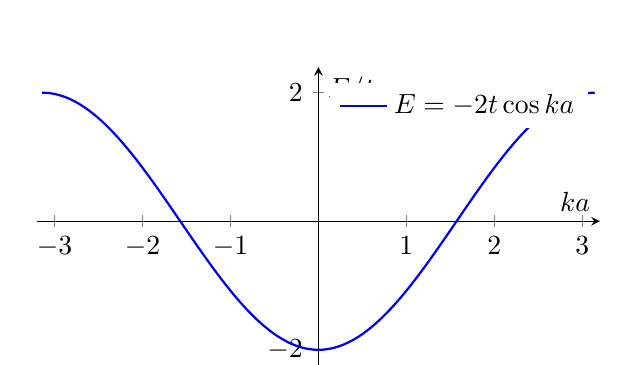
\begin{tikzpicture}
\begin{axis}[width=0.72\textwidth,height=5.5cm,
xlabel={$ka$},ylabel={$E/t$},xmin=-3.2,xmax=3.2,ymin=-2.4,ymax=2.4,
axis lines=middle,samples=160,legend style={draw=none,at={(0.98,0.95)},anchor=north east}]
\addplot[blue,thick,domain=-3.1416:3.1416] {-2*cos(deg(x))};
\addlegendentry{$E=-2t\cos ka$}
\end{axis}
\end{tikzpicture}
\caption{一维最近邻紧束缚能带。带底与带顶曲率符号相反，因而有效质量符号不同。}
\end{figure}

\begin{examplebox}
\textbf{一维二聚化链。}胞内、胞间跃迁为 $t_1,t_2$，
\[
H(k)=\begin{pmatrix}0&t_1+t_2e^{-ika}\\
t_1+t_2e^{ika}&0\end{pmatrix},
\quad E_\pm=\pm|t_1+t_2e^{ika}|.
\]
在 $k=\pi/a$ 的能隙为 $2|t_1-t_2|$。当 $t_1=t_2$，二聚化消失且能隙关闭；这既是 Peierls 图像，也是 SSH 拓扑转变的起点。
\end{examplebox}

\section{态密度与 Van Hove 奇点}
一般能带的态密度
\[
g(E)=\sum_n\int_{\rm BZ}\frac{V\dd^dk}{(2\pi)^d}
\delta[E-E_n(\vb k)].
\]
利用 $\delta$ 函数换元可写为等能面积分
\[
\boxed{g(E)=\sum_n\frac{V}{(2\pi)^d}
\int_{E_n(\vb k)=E}\frac{\dd S}{|\nabla_{\vb k}E_n|}}.
\]
当群速度 $\nabla_kE$ 在极值或鞍点为零时，态密度出现 Van Hove 奇性。一维抛物线带边
$g(E)\propto(E-E_c)^{-1/2}$ 发散；二维抛物线为常数；三维为
$\sqrt{E-E_c}$。二维鞍点常给对数发散，可增强密度波、磁性或超导不稳定性。

\section{三维晶格动力学}
令原胞 $l$ 中第 $\kappa$ 个原子位移为 $u_\alpha(l\kappa)$，谐近似势能
\[
V=\frac12\sum_{l\kappa\alpha,l'\kappa'\beta}
\Phi_{\alpha\beta}(l\kappa,l'\kappa')
u_\alpha(l\kappa)u_\beta(l'\kappa').
\]
代入平面波
\[
u_\alpha(l\kappa,t)=\frac{e_{\kappa\alpha}(\vb q)}
{\sqrt{M_\kappa}}e^{i(\vb q\cdot\vb R_l-\omega t)}
\]
得到动力学矩阵本征问题
\[
\sum_{\kappa'\beta}D_{\kappa\alpha,\kappa'\beta}(\vb q)
e_{\kappa'\beta}=\omega^2(\vb q)e_{\kappa\alpha},
\]
\[
D_{\kappa\alpha,\kappa'\beta}(\vb q)=
\frac1{\sqrt{M_\kappa M_{\kappa'}}}
\sum_{l'}\Phi_{\alpha\beta}(0\kappa,l'\kappa')
e^{i\vb q\cdot(\vb R_{l'}-\vb R_0)}.
\]
每个含 $r$ 个原子的三维原胞有 $3r$ 支：三条声学支和 $3r-3$ 条光学支。声学和规则来自均匀平移不改变能量，保证 $\vb q=0$ 有三个零频模。

量子化位移为
\[
\vb u(l\kappa)=\frac1{\sqrt N}\sum_{\vb q s}
\sqrt{\frac{\hbar}{2M_\kappa\omega_{\vb q s}}}
\vb e_{\kappa s}(\vb q)
(a_{\vb q s}+a_{-\vb q s}^\dagger)
e^{i\vb q\cdot\vb R_l}.
\]
偏振矢量说明原胞内各原子的相对运动，散射实验强度不仅取决于 $\omega$，还取决于偏振与原子散射长度。

\section{电子--声子耦合与电阻温度依赖}
离子位移调制电子周期势，最低阶耦合写成
\[
H_{e-ph}=\sum_{\vb k\vb q s}g_{\vb q s}
c_{\vb k+\vb q}^\dagger c_{\vb k}
(a_{\vb q s}+a_{-\vb q s}^\dagger).
\]
它允许电子吸收或发射声子并改变晶体动量。高温 $T\gtrsim\Theta_D$ 时声子数约正比于 $T$，金属电阻常近似线性；低温只剩小 $q$ 声子，输运还额外抑制小角散射，三维洁净金属出现 Bloch--Grüneisen
$\rho\propto T^5$。杂质给近似温度无关的残余电阻。

\begin{pitfallbox}
Matthiessen 规则 $\rho\simeq\rho_0+\rho_{ph}$ 是独立散射、单一能带等近似下的经验加和，并非严格定理。强各向异性、多带或相干散射时可能失效。
\end{pitfallbox}

\section{Boltzmann 方程与弛豫时间近似}
分布函数 obey
\[
\pdv f t+\dot{\vb r}\cdot\nabla_{\vb r}f
+\dot{\vb k}\cdot\nabla_{\vb k}f
=\left(\pdv f t\right)_{\rm coll}.
\]
均匀稳态、电场作用且
$\hbar\dot{\vb k}=-e\vb E$。取弛豫时间近似
\[
\left(\pdv f t\right)_{\rm coll}=-\frac{f-f_0}{\tau},
\]
令 $f=f_0+\delta f$，保留一阶：
\[
\delta f=e\tau\,\vb E\cdot\vb v
\left(-\pdv{f_0}{E}\right).
\]
电流
\[
j_\alpha=-e\sum_n\int\frac{\dd^3k}{(2\pi)^3}
v_\alpha\delta f
=\sigma_{\alpha\beta}E_\beta,
\]
\[
\boxed{\sigma_{\alpha\beta}=e^2\sum_n\int\frac{\dd^3k}{(2\pi)^3}
\tau_{n\vb k}v_\alpha v_\beta
\left(-\pdv{f_0}{E}\right)}.
\]
$-\partial_Ef_0$ 像宽度 $\kb T$ 的窗口，明确显示输运只取样费米面附近。

\begin{examplebox}
\textbf{恢复 Drude 公式。}各向同性抛物线带中 $\tau$ 为常数，角平均
$\langle v_x^2\rangle=v^2/3$。零温窗口变为
$\delta(E-E_F)$，积分可化为
$\sigma=ne^2\tau/m$。因此 Drude 结果并非只能靠经典碰撞图像，也能由量子统计的 Boltzmann 理论得到。
\end{examplebox}

\section{Hall 效应、多带与磁阻}
有磁场时
\[
\hbar\dot{\vb k}=-e(\vb E+\vb v\times\vb B).
\]
单一各向同性电子带给
$R_H=-1/ne$。若同时有电子和空穴，弱场两带模型
\[
R_H=\frac{p\mu_h^2-n\mu_e^2}
{e(p\mu_h+n\mu_e)^2}.
\]
Hall 符号因此取决于密度和迁移率，不能简单等同于“费米面是电子型还是空穴型”。磁阻反映轨道弯曲、多带补偿、散射各向异性，也可能含弱局域化或自旋散射。

\section{热输运与 Wiedemann--Franz 定律}
温度梯度驱动费米面附近高能粒子从热端向冷端扩散。对弹性散射、简并自由电子，
\[
\kappa=\frac{\pi^2}{3}\frac{n\kb^2T\tau}{m},
\qquad \sigma=\frac{ne^2\tau}{m},
\]
所以
\[
\boxed{\frac{\kappa}{\sigma T}=L_0=
\frac{\pi^2}{3}\left(\frac{\kb}{e}\right)^2}.
\]
这说明热流和电流由相同准粒子承担。强非弹性散射、声子热导、非费米液体或中性激发会使 Lorenz 数偏离 $L_0$。

\section{Pauli 顺磁与 Landau 抗磁}
弱磁场使自旋上下能带相对移动 $\pm\mu_BB$。费米面处转移粒子数约
$g(E_F)\mu_BB$，磁化
\[
M=\mu_B(N_\uparrow-N_\downarrow)
\quad\Rightarrow\quad
\chi_P=\mu_0\mu_B^2g(E_F)
\]
（$g$ 取总态密度时需注意因子约定）。它近似与温度无关，因为只涉及费米面态。

轨道磁场把平面运动量子化成 Landau 能级
\[
E_{n,k_z}=\hbar\omega_c(n+\tfrac12)
+\frac{\hbar^2k_z^2}{2m},
\quad\omega_c=eB/m.
\]
能级随场变化产生抗磁响应。三维自由电子在简单极限下
$\chi_L=-\chi_P/3$。晶体中有效质量、Berry 曲率和多带耦合可显著修改轨道磁性。

\section{量子振荡与费米面}
Landau 能级扫过费米能时，态密度和电阻周期振荡。Onsager 关系
\[
\boxed{F=\frac{\hbar}{2\pi e}A_{\rm ext}},\qquad
\Delta(1/B)=1/F,
\]
把振荡频率 $F$ 与垂直磁场的费米面极值截面积 $A_{\rm ext}$ 相连。温度衰减给回旋有效质量，Dingle 因子给量子寿命，振荡相位可含 Berry 相位信息。

\section{面试总结与自测}
\begin{interviewbox}
\textbf{怎样从一个能带 $E_n(\vb k)$ 推到可观测量？}
先求群速度和曲率；等能面积分给态密度；费米面窗口加散射时间给电导；磁场下半经典轨道或 Landau 量子化给 Hall、磁阻与量子振荡。强调“色散本身还不够，输运还需要占据和散射”。
\end{interviewbox}
\begin{selftestbox}
\begin{enumerate}
\item Kronig--Penney 方程中为何右边超出 $[-1,1]$ 就是禁带？
\item 什么时候两个能带可以真正交叉而非避免交叉？
\item 推导一、二、三维抛物线带边态密度。
\item 三维 $r$ 原子原胞为何有 $3r$ 条声子支？
\item 声学和规则如何约束动力学矩阵？
\item 推导弛豫时间近似下的 $\delta f$。
\item 为什么电导是费米面性质？
\item 两带 Hall 系数为什么可能改变符号？
\item Wiedemann--Franz 定律依赖哪些假设？
\item 量子振荡能测出费米面的哪些信息？
\end{enumerate}
\end{selftestbox}


\part{量子材料与计算}
\label{part:quantum-materials}
\renewcommand{\currentparttitle}{量子材料与计算}
\chapter{量子材料理论专题}

\begin{prereqbox}
Bloch 能带、二次量子化、Fermi/Bose 统计、角动量与微扰论。本章追求面试可解释深度：能写出最小模型、说明序参量或拓扑量、给出可观测后果，并明确近似边界。
\end{prereqbox}
\begin{mapbox}
\[
\text{电子相互作用}\to
\begin{cases}
\text{屏蔽与 Fermi 液体}\\
\text{Mott、磁性与密度波}\\
\text{配对与超导}
\end{cases}
\]
\[
\text{波函数几何}+\text{对称性}
\to\text{Berry 曲率、拓扑数、边界态}.
\]
“强关联”和“拓扑”回答不同问题：前者关心相互作用能否破坏单粒子图像，后者关心量子态整体几何能否连续变为平庸态；二者可以共存。
\end{mapbox}

\section{电子气、Hartree--Fock 与屏蔽}
连续电子气的 Hamiltonian
\[
H=\sum_{\vb k\sigma}\epsilon_{\vb k}
c_{\vb k\sigma}^\dagger c_{\vb k\sigma}
+\frac1{2V}\sum_{\vb q\ne0}v(q)\rho_{\vb q}\rho_{-\vb q},
\]
$v(q)=e^2/\varepsilon_0q^2$，均匀正背景抵消 $\vb q=0$ 发散。

Hartree--Fock 用 Slater 行列式近似多体态。Hartree 项是平均电荷产生的直接势，均匀电子气中被背景抵消；Fock 项来自费米反对称性，只作用于同自旋并降低能量。它能解释交换能，却缺少动态关联和有效屏蔽。

外势引起
$\delta n(q)=\chi_0(q)V_{\rm tot}(q)$，而
$V_{\rm tot}=V_{\rm ext}+v(q)\delta n$。解得
\[
V_{\rm tot}(q)=\frac{V_{\rm ext}(q)}
{1-v(q)\chi_0(q)}
\equiv\frac{V_{\rm ext}(q)}{\varepsilon(q)}.
\]
长波静态 Thomas--Fermi 近似给
\[
\varepsilon(q)=1+\frac{q_{\rm TF}^2}{q^2},\qquad
V(r)\propto\frac{e^{-q_{\rm TF}r}}r.
\]
金属自由载流子重新排列，把长程 Coulomb 势变为屏蔽势。绝缘体缺少费米面载流子，静态长波屏蔽机制不同。

\section{Lindhard 响应的结构}
非相互作用费米气的密度响应为
\[
\chi_0(\vb q,\omega)=
\sum_{\vb k}\frac{f(\epsilon_{\vb k})-
f(\epsilon_{\vb k+\vb q})}
{\hbar\omega+\epsilon_{\vb k}-\epsilon_{\vb k+\vb q}+i0^+}.
\]
分子描述粒子--空穴激发的占据差，分母描述能量代价。虚部在允许粒子--空穴连续谱内非零，对应吸收；实部控制屏蔽和集体模。RPA 条件
$\varepsilon(q,\omega)=0$ 给等离激元。三维长波极限
\[
\omega_p=\sqrt{\frac{ne^2}{m\varepsilon_0}},
\]
其 $q\to0$ 频率有限，源于长程 Coulomb 恢复力。

\section{Hubbard 模型与 Mott 绝缘体}
最小局域关联模型
\[
\boxed{H=-t\sum_{\langle ij\rangle\sigma}
(c_{i\sigma}^\dagger c_{j\sigma}+\mathrm{h.c.})
+U\sum_i n_{i\uparrow}n_{i\downarrow}}.
\]
$t$ 倾向电子离域形成能带，$U$ 惩罚双占据并倾向局域化。半填充时，$U=0$ 通常给金属；$U\gg t$ 时移动电子必然暂时制造双占据，电荷激发代价约 $U$，可成为 Mott 绝缘体，即使单粒子能带理论预测部分填充。

\subsection{强耦合映射到 Heisenberg 模型}
两个相邻格点各一个电子。直接一阶跃迁离开低能子空间，因为会形成一个空位和一个双占据，能量升高 $U$。二阶虚过程“跳过去再跳回来”给能量修正尺度 $t^2/U$。

自旋平行时 Pauli 原理阻止进入同一单轨道；反平行的自旋单态可通过双占据虚态降低能量。严格投影得到
\[
H_{\rm eff}=J\sum_{\langle ij\rangle}
\left(\vb S_i\cdot\vb S_j-\frac14n_in_j\right),
\qquad\boxed{J=\frac{4t^2}{U}>0}.
\]
在每点一个电子的子空间，密度项是常数，剩下反铁磁 Heisenberg 模型。这说明交换相互作用可以由电子的动能和 Pauli 原理共同产生。

\begin{examplebox}
\textbf{Hubbard 二聚体。}两电子半填充时，三重态不能通过跃迁混入双占据，能量近似不降；单态与双占据态耦合，二阶能量降低约 $-4t^2/U$。因此单态更低，单重--三重劈裂就是 $J$。
\end{examplebox}

\section{磁有序、挫折与自旋波}
Heisenberg 模型
$H=J\sum_{\langle ij\rangle}\vb S_i\cdot\vb S_j$（本节采用 $J>0$ 反铁磁约定）。若晶格几何使所有键不能同时取最低能，就产生几何挫折，如三角格反铁磁。若不同相互作用竞争，也可有交换挫折。

铁磁基态附近用 Holstein--Primakoff 变换
\[
S_i^z=S-a_i^\dagger a_i,\quad
S_i^+\simeq\sqrt{2S}\,a_i,\quad
S_i^-\simeq\sqrt{2S}\,a_i^\dagger.
\]
保留二次项后得到自由玻色子磁振子。各向同性交换铁磁体长波
$\omega\propto q^2$；反铁磁体有两个子格，经 Bogoliubov 变换得到长波线性色散。磁振子是自旋有序背景的集体激发。

量子自旋液体不是“自旋方向随机”的高温顺磁体，而是零温无常规磁长程序、仍有强量子纠缠和分数量子激发的基态。仅凭“没有磁峰”不能确证，还需排除无序、弱矩或动力学缓慢等普通解释。

\section{Peierls 不稳定性与密度波}
一维半填充金属有 $2k_F$ 嵌套：把右费米点平移 $2k_F$ 与左费米点重合。周期为 $\pi/k_F$ 的晶格畸变耦合 $\pm k_F$ 态并在费米能开隙，电子能降低。弹性能升高与电子能降低竞争；一维费米面响应在 $2k_F$ 特别强，使任意弱耦合也可能不稳定。

电荷密度波写成
\[
\rho(\vb r)=\rho_0+\mathrm{Re}[
\rho_{\vb Q}e^{i\vb Q\cdot\vb r}],
\]
自旋密度波把标量 $\rho_{\vb Q}$ 换成自旋矢量。其成因可能是费米面嵌套、电子--声子耦合或电子关联。实验上应综合超晶格峰、能隙、声子软化和局域谱，而非把所有周期调制都归于同一机制。

\section{Berry 相位、连接与曲率}
若 Hamiltonian 缓慢依赖参数 $\vb R$，绝热演化的本征态除动力学相位外还积累
\[
\gamma_n=\oint_{\mathcal C}
\vb{\mathcal A}_n(\vb R)\cdot\dd\vb R,\qquad
\vb{\mathcal A}_n=i\langle n|\nabla_{\vb R}n\rangle.
\]
改变局域相位
$|n\rangle\to e^{i\chi(\vb R)}|n\rangle$ 时
$\vb{\mathcal A}\to\vb{\mathcal A}-\nabla\chi$，连接依赖规范；曲率
\[
\vb\Omega_n=\nabla_{\vb R}\times\vb{\mathcal A}_n
\]
规范不变。闭合回路相位只模 $2\pi$ 有意义。

在二维布里渊区
\[
\boxed{C_n=\frac1{2\pi}\int_{\rm BZ}\Omega_{n,z}(\vb k)\dd^2k}
\]
为第一 Chern 数。由于布里渊区是闭合流形，光滑规范拼接条件使积分量子化为整数。满带 Hall 电导
\[
\sigma_{xy}=C\frac{e^2}{h}.
\]

\begin{whybox}
拓扑不变量为何必须在能隙关闭时才能改变？只要占据带与空带之间始终有隙，本征投影可随参数光滑变化，整数 $C$ 不可能连续改变。改变拓扑类必须让波函数失去全局光滑定义，通常对应体能隙关闭或相关对称性被破坏。
\end{whybox}

\section{二能带模型与 Dirac 点}
一般二能带 Hamiltonian
\[
H(\vb k)=d_0(\vb k)I+\vb d(\vb k)\cdot\vb\sigma,
\qquad E_\pm=d_0\pm|\vb d|.
\]
能隙关闭要求 $\vb d=0$。归一化
$\hat{\vb d}(\vb k)$ 把布里渊区映射到 Bloch 球，Berry 曲率衡量该映射的局域扭转，Chern 数计数覆盖次数。

二维 Dirac Hamiltonian
\[
H=v(k_x\sigma_x+k_y\sigma_y)+m\sigma_z
\]
有谱
$E_\pm=\pm\sqrt{v^2k^2+m^2}$。$m$ 是质量项并打开 $2|m|$ 的隙；不同对称性限制哪些质量项允许。质量变号的界面可产生局域边界态，这是体边对应的最简连续图像。

\begin{figure}[htbp]
\centering
\begin{tikzpicture}[scale=1.05]
\draw[->] (-3,0)--(3.2,0) node[right] {$k$};
\draw[->] (0,-3)--(0,3.2) node[above] {$E$};
\draw[blue,thick,domain=-2.7:2.7,samples=100] plot (\x,{sqrt(\x*\x+0.55)});
\draw[red,thick,domain=-2.7:2.7,samples=100] plot (\x,{-sqrt(\x*\x+0.55)});
\draw[<->] (0,{-sqrt(0.55)})--(0,{sqrt(0.55)}) node[midway,right] {$2|m|$};
\node at (1.75,2.45) {导带};
\node at (1.75,-2.35) {价带};
\end{tikzpicture}
\caption{有质量 Dirac 模型的能隙。拓扑转变中质量变号通常伴随 $m=0$ 处体能隙关闭。}
\end{figure}

\section{SSH 模型与一维体边对应}
SSH Bloch Hamiltonian
\[
H(k)=[t_1+t_2\cos ka]\sigma_x+
[t_2\sin ka]\sigma_y.
\]
$\vb d(k)$ 位于赤道。若 $|t_2|>|t_1|$，随 $k$ 绕原点一周，绕数为 1；若
$|t_1|>|t_2|$，绕数为 0。开边界且截断方式固定时，非平庸相出现端态。

\begin{figure}[htbp]
\centering
\begin{tikzpicture}[scale=1.0,>=Latex]
\foreach \x in {0,2,4,6}{
  \fill[blue] (\x,0) circle (2.5pt);
  \fill[red] (\x+0.8,0) circle (2.5pt);
  \draw[very thick] (\x+0.08,0)--(\x+0.72,0);
}
\foreach \x in {0,2,4}{
  \draw[thick,dashed] (\x+0.88,0)--(\x+1.92,0);
}
\node[below] at (0.4,-0.1) {$t_1$};
\node[below] at (1.4,-0.1) {$t_2$};
\node[right] at (6.9,0) {开边界};
\end{tikzpicture}
\caption{SSH 二聚化链。胞内和胞间跃迁的相对大小决定绕数与端态。}
\end{figure}

端态能量钉在零附近依赖手征/亚晶格对称性；破坏该对称性可移动端态能量，但只要保护条件和体隙保持，拓扑差异仍以适当形式存在。回答“有边界态所以拓扑”不充分，还要说明保护对称性与体不变量。

\section{石墨烯、拓扑绝缘体与量子 Hall}
石墨烯蜂窝格由两个子格组成，最近邻紧束缚在 $K,K'$ 点产生 Dirac 锥。低能
\[
H_\tau=\hbar v_F(\tau q_x\sigma_x+q_y\sigma_y),
\]
$\tau=\pm1$ 标记谷。子格势差产生 $\sigma_z$ 质量并开平庸隙；特定时间反演破缺的复次近邻跃迁可产生 Chern 绝缘体。

二维量子自旋 Hall 可看作时间反演伙伴的两份相反 Chern 系统，总电荷 Chern 数为零但边缘态成 Kramers 对。三维拓扑绝缘体体内有隙、表面有奇数个 Dirac 锥；非磁无序不能单粒子弹性后向散射一个孤立 Kramers 对。强磁性可破坏时间反演并打开表面隙。

\section{BCS 平均场与 Bogoliubov 准粒子}
简化配对 Hamiltonian
\[
H=\sum_{\vb k\sigma}\xi_{\vb k}c_{\vb k\sigma}^\dagger c_{\vb k\sigma}
-\sum_{\vb k\vb k'}V_{\vb k\vb k'}
c_{\vb k\uparrow}^\dagger c_{-\vb k\downarrow}^\dagger
c_{-\vb k'\downarrow}c_{\vb k'\uparrow}.
\]
定义序参量
\[
\Delta_{\vb k}=-\sum_{\vb k'}V_{\vb k\vb k'}
\langle c_{-\vb k'\downarrow}c_{\vb k'\uparrow}\rangle.
\]
平均场分解后，每个 $(\vb k,-\vb k)$ 子空间写成 Nambu 矩阵
\[
H_{\vb k}=
\begin{pmatrix}c_{\vb k\uparrow}^\dagger&
c_{-\vb k\downarrow}\end{pmatrix}
\begin{pmatrix}\xi_{\vb k}&\Delta_{\vb k}\\
\Delta_{\vb k}^*&-\xi_{\vb k}\end{pmatrix}
\binom{c_{\vb k\uparrow}}{c_{-\vb k\downarrow}^\dagger}.
\]
幺正 Bogoliubov 变换给
\[
\boxed{E_{\vb k}=\sqrt{\xi_{\vb k}^2+|\Delta_{\vb k}|^2}}.
\]
对常数吸引 $V$ 和 Debye 壳层，零温能隙方程
\[
1=VN(0)\int_0^{\hbar\omega_D}
\frac{\dd\xi}{\sqrt{\xi^2+\Delta^2}}
\]
在弱耦合给
\[
\Delta(0)\simeq2\hbar\omega_D
e^{-1/VN(0)},\qquad
2\Delta(0)/\kb T_c\simeq3.53.
\]
指数非解析性体现费米面对任意弱吸引的不稳定。

\begin{examplebox}
\textbf{相干因子。}Bogoliubov 准粒子
$\gamma_{\vb k\uparrow}=u_{\vb k}c_{\vb k\uparrow}
-v_{\vb k}c_{-\vb k\downarrow}^\dagger$，
\[
|u_k|^2=\frac12\left(1+\frac{\xi_k}{E_k}\right),\quad
|v_k|^2=\frac12\left(1-\frac{\xi_k}{E_k}\right).
\]
远高于费米面 $u^2\to1$，准粒子像电子；远低于费米面 $v^2\to1$，更像空穴；费米面处两者等混合。
\end{examplebox}

\section{非常规与拓扑超导的面试边界}
常规 $s$ 波通常各向同性、全能隙、时间反演配对；非常规超导的序参量在动量空间可能变号或有节点，如
$d_{x^2-y^2}\propto\cos k_x-\cos k_y$。节点导致低能态密度幂律，使低温比热、穿透深度和 NMR 松弛率与全能隙的指数行为不同。

拓扑超导还要求 BdG 准粒子能带具有非平庸拓扑，并在边界或缺陷承载受保护的 Majorana 模。零偏压峰只是候选证据，也可能由普通 Andreev 束缚态、无序或 Kondo 效应产生，不能单凭一张谱图下结论。

\section{DFT、Kohn--Sham 与 Wannier 工作流}
Hohenberg--Kohn 思想表明基态密度决定外势和基态性质。Kohn--Sham 辅助非相互作用系统满足
\[
\left[-\frac{\hbar^2\nabla^2}{2m}+V_{\rm ext}
+V_H[n]+V_{\rm xc}[n]\right]\phi_i
=\epsilon_i\phi_i,
\qquad n(\vb r)=\sum_{i\in{\rm occ}}|\phi_i|^2.
\]
实际自洽循环为：猜密度 $\to$ 构造有效势 $\to$ 解本征方程 $\to$ 更新密度
$\to$ 混合并判断收敛。交换关联泛函是主要近似来源。

Kohn--Sham 本征值原则上是辅助量，不等同于严格准粒子激发谱；普通局域/半局域泛函常低估带隙，强关联体系可能错误给出金属。DFT+$U$、杂化泛函、GW 或 DMFT 分别修正不同问题。

Wannier 函数由一组 Bloch 带作规范选择与 Fourier 变换：
\[
|W_{n\vb R}\rangle=\frac1N\sum_{\vb k}
e^{-i\vb k\cdot\vb R}\sum_mU_{mn}(\vb k)|\psi_{m\vb k}\rangle.
\]
它把第一性原理能带映射成局域紧束缚模型，便于插值、计算 Berry 曲率、表面态和输运。结果依赖选带窗口、投影轨道和规范，必须检查能带复现质量。

\section{三个综合例题}
\begin{examplebox}
\textbf{例 1：为什么 Mott 绝缘不能只看能带填充？}半填充单带按非相互作用理论必为金属；若 $U$ 大于带宽，加入一个电子必须产生双占据，移走一个电子产生空穴，粒子--空穴电荷激发之间出现关联能隙。自旋仍可低能波动，因此电荷绝缘不等于没有低能自由度。
\end{examplebox}

\begin{examplebox}
\textbf{例 2：Dirac 质量变号的界面态。}取
$H=-iv\sigma_x\partial_x+vk_y\sigma_y+m(x)\sigma_z$，
$m(-\infty)m(+\infty)<0$。先令 $k_y=0,E=0$，方程有
$\psi\propto\exp[-\int^xm(x')\dd x'/v]$ 的可归一化解；恢复
$k_y$ 后得到沿界面传播的线性色散。边界态来自两侧质量拓扑不同。
\end{examplebox}

\begin{examplebox}
\textbf{例 3：如何判别全能隙与节点？}不要只看一个量。全能隙低温电子比热和穿透深度呈指数抑制；线节点常给幂律态密度并导致 $C\sim T^2$（洁净三维线节点的典型结果）等。杂质会改变幂律，因此需结合热导、NMR、相位敏感实验和材料洁净度。
\end{examplebox}

\section{面试总结与自测}
\begin{interviewbox}
\textbf{强关联是什么？}不是简单指相互作用“不小”，而是相互作用使独立电子能带或微扰准粒子图像失效。Hubbard 模型中用 $U/W$ 衡量局域排斥与带宽竞争，Mott 绝缘是典型后果。

\textbf{拓扑材料为什么特殊？}占据态波函数在整个布里渊区具有不能由局域微扰连续消除的整体结构，用 Berry 曲率和拓扑不变量描述；不同拓扑相之间通常必须闭合体能隙或破坏保护对称性，并在边界产生受保护态。

\textbf{BCS 的最小回答：}费米面附近任意弱吸引导致 Cooper 不稳定；宏观相干配对产生复序参量；Bogoliubov 准粒子为电子空穴混合并具有能隙；Meissner 和相位刚度说明它是带电凝聚态。
\end{interviewbox}
\begin{selftestbox}
\begin{enumerate}
\item Hartree 与 Fock 项的来源和物理差别是什么？
\item Thomas--Fermi 屏蔽为何在金属中有效？
\item 解释 Lindhard 函数分子与分母。
\item 从 Hubbard 强耦合推导 $J=4t^2/U$ 的符号。
\item Mott 绝缘体和普通能带绝缘体怎样区分？
\item 挫折为什么可能增强量子涨落？
\item Peierls 不稳定为何在一维特别强？
\item Berry 连接与电磁矢势的规范结构有何相似？
\item Chern 数为什么是整数，何时能改变？
\item SSH 端态依赖哪些对称性和边界约定？
\item 时间反演如何约束 Berry 曲率与 Hall 电导？
\item BCS 平均场为什么使用 Nambu 空间？
\item 节点超导会怎样改变低温热力学？
\item DFT 能带与真实光电子谱为何不必相同？
\item Wannier 化在拓扑和输运计算中有何作用？
\end{enumerate}
\end{selftestbox}

\chapter{计算凝聚态：从模型到可信结果}

\begin{prereqbox}
线性代数、Bloch 定理、紧束缚和 DFT 基本概念。本章不绑定某个软件，训练研究生面试中更重要的能力：怎样把物理问题转化为计算、怎样检查结果、怎样识别数值伪影。
\end{prereqbox}
\begin{mapbox}
\[
\begin{aligned}
\text{物理问题}&\to\text{自由度与模型}\to\text{离散化/基底}\\
&\to\text{算法}\to\text{收敛与守恒检查}\to\text{可观测量}.
\end{aligned}
\]
任何漂亮图像都必须回答三个问题：对什么参数收敛？满足什么精确约束？有没有更简单的替代解释？
\end{mapbox}

\section{先选问题，再选方法}
计算方法的适用边界由自由度和纠缠结构决定：
\begin{itemize}
\item 弱关联基态电子结构：DFT、紧束缚、Wannier；
\item 小尺寸强关联模型：精确对角化；
\item 一维低纠缠基态：矩阵乘积态与 DMRG；
\item 有限温量子统计：量子 Monte Carlo，但可能有符号问题；
\item 局域动态关联：DMFT；
\item 准粒子修正和光学激发：GW、Bethe--Salpeter 等更高阶方法。
\end{itemize}
面试回答不应只报软件名，而要从系统尺度、维数、相互作用强弱和目标观测量解释选择。

\section{紧束缚数值化}
给定 $n$ 个轨道，Bloch Hamiltonian 是 $n\times n$ Hermitian 矩阵
$H(\vb k)$。基本流程：
\begin{enumerate}
\item 依据晶格、轨道和对称性列出允许跃迁；
\item 选择高对称路径画能带，但计算态密度或拓扑量必须覆盖整个布里渊区；
\item 对每个 $\vb k$ 对角化，保存本征值和本征矢；
\item 检查 $H(\vb k+\vb G)=H(\vb k)$、Hermitian 性和对称性简并；
\item 从本征矢计算轨道权重、速度、Berry 量等。
\end{enumerate}

\begin{examplebox}
\textbf{两带模型的数值检查。}若
$H=d_0I+\vb d\cdot\vb\sigma$，数值本征值必须等于
$d_0\pm|\vb d|$。这给出单元测试。若数值结果偏离，优先检查复跃迁的共轭、相位约定和 Fourier 变换符号，而不是调绘图参数。
\end{examplebox}

\section{$k$ 点采样与收敛}
周期系统把布里渊区积分离散为
\[
\int_{\rm BZ}\frac{\dd^dk}{\Omega_{\rm BZ}}f(\vb k)
\simeq\sum_{\vb k}w_{\vb k}f(\vb k).
\]
金属因费米面不连续最难收敛，常需更密 $k$ 网格和展宽。绝缘体有隙，占据随 $k$ 光滑，通常更容易。

展宽把 $\delta(E-E_n)$ 替换为 Gaussian 或 Lorentzian。展宽过小会显出离散网格尖峰，过大会抹去真实小能隙。可信做法是同时增加网格、减小展宽，寻找稳定区间。

\begin{pitfallbox}
沿高对称路径画出的“能带图”不是布里渊区采样。它适合展示色散和简并，却不能可靠计算总能、态密度、载流子浓度或 Chern 数。
\end{pitfallbox}

\section{有限尺寸与边界条件}
长度 $L$ 的周期系统动量间距
$\Delta k=2\pi/L$。临界点关联长度 $\xi$ 若接近 $L$，观测量会显著受尺寸影响。有限尺寸标度的一般形式
\[
O(L,g)=L^{-x_O/\nu}
\mathcal F[(g-g_c)L^{1/\nu}].
\]
不同尺寸曲线的交叉或数据坍缩可估计临界点和指数。

周期边界减少表面效应，开边界用于研究边缘态。拓扑端态只在开边界出现，但体拓扑不变量应由周期系统定义。若端态局域长度接近样品长度，两端杂化会产生指数小劈裂，不应误判为拓扑被破坏。

\section{精确对角化}
自旋 $1/2$ 的 $N$ 个格点 Hilbert 空间维数为 $2^N$，费米格点模型还要考虑粒子数和自旋。精确对角化的关键不是调用本征值函数，而是利用对称性分块：
\[
[H,N]=0,\quad[H,S_z]=0,\quad[H,T]=0
\]
时可在固定粒子数、磁量子数和动量扇区独立对角化。稀疏 Lanczos 算法只需矩阵--向量乘法，可求极少数低能态。

从基态 $|0\rangle$ 可求静态关联
\[
C_{ij}=\langle0|\vb S_i\cdot\vb S_j|0\rangle
\]
和结构因子
\[
S(\vb q)=\frac1N\sum_{ij}e^{i\vb q\cdot(\vb r_i-\vb r_j)}C_{ij}.
\]
有限系统没有严格自发对称性破缺，序参量平均值可能为零，应看关联函数、简并结构和尺寸标度。

\section{变分、均场与自洽}
Hartree--Fock、BCS、磁平均场都把四费米项分解为二次项和待定平均值。一般自洽循环：
\[
\Delta^{(n)}
\xrightarrow{\text{构造 }H_{\rm MF}}
\{|u_m\rangle,E_m\}
\xrightarrow{\text{求期望值}}
\Delta_{\rm out}^{(n)}
\xrightarrow{\text{混合}}
\Delta^{(n+1)}.
\]
简单线性混合
$\Delta^{(n+1)}=(1-\alpha)\Delta^{(n)}+\alpha\Delta_{\rm out}^{(n)}$。
收敛不等于找到全局最低自由能：不同初值可能落入亚稳解，应比较总能/自由能并扫描初值。

\begin{examplebox}
\textbf{Stoner 铁磁判据。}局域排斥的均场使自旋能带劈裂
$\Delta=Um$。小磁化下电子能降低与态密度有关，展开自由能二次项得到
\[
F(m)-F(0)\sim\frac12\left[\frac1{N(E_F)}-U\right]m^2.
\]
当 $UN(E_F)>1$，顺磁态不稳定。该判据说明大态密度有利于巡游铁磁，但平均场会夸大有序。
\end{examplebox}

\section{DFT 的输入、输出与收敛}
平面波赝势计算常见收敛参数：
\begin{itemize}
\item 平面波截断能：决定基底完备程度；
\item $k$ 网格：决定布里渊区积分；
\item 真空层与超胞：决定周期镜像相互作用；
\item 力和总能阈值：决定结构弛豫；
\item 展宽和占据方法：影响金属收敛；
\item 自旋、SOC、磁初态和 $U$：决定允许探索的解空间。
\end{itemize}
比较不同结构的能量差时，每个结构必须使用相同精度。若目标能差只有
$1\,\mathrm{meV}$，而截断能或 $k$ 网格误差是
$10\,\mathrm{meV}$，结论没有意义。

\section{Wannier 插值与拓扑计算}
从第一性原理选取一组目标能带，通过投影和规范优化得到局域 Wannier 轨道。检查包括：
\begin{enumerate}
\item Wannier 插值能带在目标能窗内复现原始能带；
\item 轨道中心和扩展合理；
\item 对称性与简并未被数值规范错误破坏；
\item 增减能窗或初始投影时物理结论稳定。
\end{enumerate}

离散 $k$ 网格上 Berry 相位可用相邻本征态重叠计算，而不是直接对相位不连续的本征矢作差分。单带 Wilson 环
\[
e^{i\gamma}=\prod_j
\frac{\langle u_{\vb k_j}|u_{\vb k_{j+1}}\rangle}
{|\langle u_{\vb k_j}|u_{\vb k_{j+1}}\rangle|}.
\]
多带占据子空间使用重叠矩阵的行列式或 Wilson 矩阵，保证对子空间内幺正混合不敏感。

\section{误差、验证与可重复性}
误差至少分四类：
\begin{enumerate}
\item \textbf{模型误差：}遗漏轨道、相互作用或声子；
\item \textbf{方法误差：}平均场、泛函或微扰截断；
\item \textbf{数值误差：}网格、尺寸、截断和迭代容差；
\item \textbf{统计误差：}Monte Carlo 采样和实验噪声。
\end{enumerate}
提高数值精度只能消除第三类，不能修复错误模型。可信结果应报告单位、参数、收敛曲线、对称性检查和数据处理流程。

\section{三个计算案例}
\begin{examplebox}
\textbf{案例 1：寻找拓扑转变。}
\begin{enumerate}
\item 扫描控制参数并记录直接/间接能隙；
\item 定位能隙最小的 $\vb k$，识别对称性表示或 Dirac 质量；
\item 在两侧计算 Berry/Z$_2$ 指标；
\item 开边界计算边缘谱，检查体边对应；
\item 改变网格、边界宽度和小扰动，确认稳定。
\end{enumerate}
\end{examplebox}

\begin{examplebox}
\textbf{案例 2：拟合紧束缚参数。}先明确拟合能窗与轨道；不仅拟合本征值，还比较轨道权重和对称性；用未参与拟合的路径或应变条件作交叉验证。参数高度相关时，不要给出虚假的高精度小数。
\end{examplebox}

\begin{examplebox}
\textbf{案例 3：判断磁基态。}分别从铁磁、不同反铁磁和非磁初态自洽；比较总能和局域磁矩；增大超胞检查更长周期；检查 $k$ 网格、SOC 和 $U$ 依赖。若能差接近数值误差，只能报告近简并而非确定基态。
\end{examplebox}

\begin{interviewbox}
\textbf{你如何证明计算结果可信？}先给收敛测试，再给精确约束（Hermitian、守恒、对称性、和规则），接着用可解极限或独立方法交叉验证，最后说明模型和方法仍有哪些系统误差。
\end{interviewbox}
\begin{selftestbox}
\begin{enumerate}
\item 为什么高对称路径不能替代全布里渊区积分？
\item 金属为何需要更密 $k$ 网格？
\item 怎样区分有限尺寸隙和真实体隙？
\item 精确对角化为什么必须利用对称性？
\item 有限系统如何判断自发有序倾向？
\item 自洽收敛为什么不等于全局最低能？
\item DFT 总能差需要哪些共同收敛条件？
\item 为什么直接差分本征矢相位可能得到错误 Berry 曲率？
\item 四类误差中哪些不能靠更严格容差消除？
\item 最小的可重复计算记录应包括什么？
\end{enumerate}
\end{selftestbox}


\part{实验、面试训练与附录}
\label{part:interview}
\renewcommand{\currentparttitle}{实验、面试训练与附录}
\chapter{量子材料实验与数据阅读}

\begin{prereqbox}
理解倒空间、态密度、费米面、线性响应和基本相变。本章不训练仪器操作，而训练“测量量是什么、怎样从数据到物理结论、替代解释是什么”。
\end{prereqbox}
\begin{mapbox}
\[
\begin{array}{c|c}
\text{问题}&\text{常用探针}\\\hline
\text{原子/磁结构}&X\text{ 射线、中子、电子衍射}\\
\text{占据能带 }E(\vb k)&\text{ARPES}\\
\text{局域态密度}&\text{STM/STS}\\
\text{费米面与散射}&\text{输运、量子振荡}\\
\text{体相能隙与激发}&\text{比热、磁化率、光学、NMR}
\end{array}
\]
\end{mapbox}

\section{衍射：从峰位和强度到结构}
弹性散射满足
$\vb Q=\vb k_f-\vb k_i=\vb G$。峰位给晶格周期和对称性，强度
\[
I(\vb G)\propto
\left|\sum_j f_j(\vb G)e^{-i\vb G\cdot\vb r_j}\right|^2
\]
给基元信息。有限晶粒尺寸导致峰展宽，热振动给 Debye--Waller 衰减，无序产生弥散散射。

X 射线主要看电子密度，重元素更强；中子核散射长度不随原子序数单调，能看轻元素和同位素，且中子磁矩可测磁结构；电子散射强，适合薄样品和局域结构但多重散射更显著。

\begin{examplebox}
若降温后在原晶格禁戒位置出现新峰，先判断其波矢 $\vb Q$：整数/半整数超结构峰可提示晶格倍周期、磁序或电荷序。必须比较 X 射线与中子、是否有偏振分析，以及峰强随温度的序参量行为，不能仅凭“多了一个峰”断言具体序。
\end{examplebox}

\section{非弹性散射：测量动力学结构因子}
能量和动量同时转移时测得
\[
S(\vb Q,\omega)=\frac1{2\pi N}
\int\dd t\,e^{i\omega t}
\langle\rho_{\vb Q}(t)\rho_{-\vb Q}(0)\rangle.
\]
它是密度或自旋关联函数的频谱。峰的位置给激发色散，宽度给寿命，积分强度给谱权重。声子、磁振子和连续粒子--空穴激发可由其 $\vb Q$ 依赖、偏振和温度行为区分。

\section{ARPES：能量与动量分辨的占据谱}
光电效应给
\[
E_{\rm kin}=h\nu-\phi-E_B.
\]
平行表面的晶体动量近似守恒：
\[
k_\parallel=\frac{\sqrt{2mE_{\rm kin}}}{\hbar}\sin\theta.
\]
在突然近似和矩阵元框架下
\[
I(\vb k,\omega)\propto |M_{fi}|^2
A(\vb k,\omega)f(\omega).
\]
$A$ 是单粒子谱函数，$f$ 说明 ARPES 主要看占据态。峰位置给重整化色散，峰宽与自能虚部和寿命相关，强度还受光子能量、偏振、轨道选择定则与表面条件影响。

\begin{pitfallbox}
ARPES 不是“直接拍到裸能带”。实验强度包含矩阵元、分辨率、背景和 Fermi 函数；强关联时峰可能不再对应长寿命准粒子。表面态与体态可通过光子能量导致的 $k_z$ 色散、样品终止面和计算比较来区分。
\end{pitfallbox}

\section{STM/STS：实空间与局域谱}
弱隧穿、针尖态密度平坦时，Tersoff--Hamann 图像给
\[
I(V)\propto\int_0^{eV}\rho_s(\vb r,E_F+\epsilon)\dd\epsilon,
\qquad
\frac{\dd I}{\dd V}\propto\rho_s(\vb r,E_F+eV).
\]
恒流形貌是几何高度与积分态密度的混合，不是纯粹原子高度。STS 的
$\dd I/\dd V$ 近似局域态密度，可看超导相干峰、能隙、杂质束缚态和 Landau 能级。

准粒子干涉中，缺陷把 $\vb k$ 散射到 $\vb k'$，实空间态密度出现
$\vb q=\vb k'-\vb k$ 调制；Fourier 变换可反推等能轮廓和选择定则。缺失某散射矢量可能来自自旋纹理或矩阵元，但也可能是信噪比和无序。

\section{直流输运：电阻、Hall 与磁阻}
金属通常降温电阻下降，绝缘行为常表现为 $\dd\rho/\dd T<0$，但这不是严格相定义。超导转变要看零电阻、抗磁和热力学证据；仅有电阻下降可能是丝状通道。

Hall 斜率在单带模型给载流子符号和密度，多带时需拟合
$\rho_{xy}(B)$ 与纵向磁阻。反常 Hall 可写
\[
\rho_{xy}=R_0B+R_sM,
\]
第二项与磁化、Berry 曲率和散射机制有关。非线性 Hall 不自动证明多带，也可能含磁性或几何混合。

\section{量子振荡}
Shubnikov--de Haas 测电阻振荡，de Haas--van Alphen 测磁化振荡。对 $1/B$ 作 Fourier 变换得到频率和费米面极值面积。Lifshitz--Kosevich 温度因子
\[
R_T=\frac{X}{\sinh X},\qquad
X=\frac{2\pi^2\kb Tm^*}{\hbar eB}
\]
可拟合回旋质量；场依赖衰减给 Dingle 温度和量子寿命。Landau fan 截距与 Berry 相位有关，但 Zeeman、三维曲率和索引约定都会改变相位判断。

\section{比热、磁化率和热导}
连续相变常在比热出现跳变或 $\lambda$ 异常。超导弱耦合 BCS 有
$\Delta C/\gamma T_c\simeq1.43$；偏离可来自强耦合、多带、节点或样品体积分数。

零场冷却与场冷却磁化可看屏蔽和磁通钉扎。Curie 尾可能来自少量顺磁杂质，不应直接解释为本征磁性。热导由电子、声子和其他中性激发共同承担，结合 Wiedemann--Franz 与场依赖可分离通道。

\section{光学、Raman 与泵浦探测}
反射率经 Kramers--Kronig 可得复电导。Drude 峰看自由载流子，有限频率峰可来自带间跃迁、声子、激子或关联激发。总谱权重满足光学和规则；谱权重跨较大能标转移是关联的重要线索。

Raman 散射近似零动量转移，可按偏振选择晶格对称通道；泵浦--探测先把系统推离平衡，再追踪序参量、准粒子和集体模的恢复时间。非平衡信号不一定等于平衡能带简单加热。

\section{四类读图模板}
\begin{examplebox}
\textbf{判断超导。}电阻到仪器零值；低场磁化出现体抗磁；比热在同一 $T_c$ 有异常；隧穿或光学见能隙。若只有其中一项，应主动列出接触、丝状相、磁杂质或结构转变等替代解释。
\end{examplebox}
\begin{examplebox}
\textbf{判断磁相变。}磁化率出现 cusp 或发散、比热异常、中子出现磁 Bragg 峰。铁磁还看自发磁化和磁滞；反铁磁可能净磁矩为零，不能因磁化小而排除。
\end{examplebox}
\begin{examplebox}
\textbf{判断金属--绝缘跨越。}结合 $\rho(T)$、Hall、光学 Drude 权重、ARPES 是否有费米面及低温极限。局域化、能隙、颗粒效应和接触问题都可产生上翘电阻。
\end{examplebox}
\begin{examplebox}
\textbf{判断拓扑表面态。}ARPES 看跨越体隙的表面色散和自旋纹理，STS 看缺陷散射与 Landau 能级，输运看二维通道和量子化响应。任何单一“Dirac 锥”都不足以替代拓扑不变量与对称性分析。
\end{examplebox}

\begin{selftestbox}
\begin{enumerate}
\item 衍射峰位、强度、宽度分别告诉什么？
\item X 射线和中子对磁结构的能力有何不同？
\item $S(\vb Q,\omega)$ 与关联函数有何联系？
\item ARPES 强度为何不等于谱函数本身？
\item STM 形貌为什么不是纯几何高度？
\item 单带 Hall 分析何时失效？
\item 量子振荡怎样得到有效质量？
\item 怎样用三类证据确认体超导？
\item 比热、磁化率、输运对相变各有什么盲区？
\item 面对一张“漂亮数据图”，如何系统列出替代解释？
\end{enumerate}
\end{selftestbox}


\chapter{综合高频面试题}
\newcommand{\qa}[5]{\subsection{#1}\textbf{考察点：}#2\par
\textbf{标准回答：}#3\par\textbf{追问方向：}#4\par
\textbf{常见错误：}#5\par}

\qa{为什么要引入倒格子？}{周期性、傅里叶空间。}
{周期晶格上的函数可按倒格矢展开；衍射条件是动量转移等于倒格矢，Bloch 准动量也只在模倒格矢意义下不同。倒格子把平移对称性变成代数关系。}
{第一布里渊区；晶面间距 $d=2\pi/G$。}{只说“计算方便”，不说明周期相位。}

\qa{Bloch 定理的物理意义是什么？}{平移对称性与准动量。}
{因 $[H,T_{\vb R}]=0$，本征态可同时取为平移本征态，故 $\psi=\ee^{i\vb k\cdot\vb r}u_{\vb k}$。电子受周期势作用，但保留平面波式平移相位，$\hbar\vb k$ 是晶体准动量。}
{$\vb k$ 与 $\vb k+\vb G$；能带指标。}{把 $u_{\vb k}$ 当常数，误称电子完全自由。}

\qa{能隙为什么在布里渊区边界打开？}{Bragg 反射与简并微扰。}
{区边界自由电子态 $|\vb k\rangle,|\vb k-\vb G\rangle$ 简并；周期势 $V_G$ 耦合它们，二阶矩阵本征值为 $E_0+V_0\pm|V_G|$，开隙 $2|V_G|$。}{驻波密度；高维 Bragg 面。}{只说“周期势造成”而不给简并与耦合。}

\qa{声学支和光学支的区别是什么？}{原胞内相位与 $k=0$。}
{长波声学支中原胞内原子同相运动且 $\omega\to0$；光学支反相运动，$k=0$ 仍有恢复力和有限频率。极性晶体的光学模可产生偶极矩并与红外光耦合。}{LO--TO 劈裂；原胞原子数与分支数。}{声称所有光学支都必与可见光强耦合。}

\qa{为什么低温声子热容是 $T^3$？}{态密度与 Bose 分布。}
{三维线性色散给 $g(\omega)\propto\omega^2$；能量积分换元 $x=\hbar\omega/\kb T$ 后 $U\propto T^4$，故 $C_V\propto T^3$，适用 $T\ll\Theta_D$。}{二维/一维指数；Debye 截止。}{把 $T^3$ 归因于“有三个偏振”。}

\qa{为什么电子热容是 $T$？}{费米面薄壳层。}
{Pauli 原理使深层电子无法改变占据，只有距 $E_F$ 约 $\kb T$ 的态参与；参与数 $\propto T$，每个激发能标度 $\propto T$，能量增量 $\propto T^2$，所以热容线性。}{Sommerfeld 系数；有效质量。}{用经典均分定理。}

\qa{Drude 模型为什么失败？}{经典统计与能带缺失。}
{它能给 $\sigma=ne^2\tau/m$ 与简单 Hall 效应，但采用经典粒子和经验碰撞时间，不能解释电子热容、某些正 Hall 系数及复杂温度依赖；Sommerfeld 统计和能带理论分别修正这些缺陷。}{平均自由程；Matthiessen 规则。}{说它“完全错误”。}

\qa{费米面有什么物理意义？}{低能激发边界。}
{它是零温占据态在 $k$ 空间的边界；低温输运、热容和磁响应主要由其附近态及速度、曲率决定，而不只由总电子数决定。}{Luttinger 定理；费米面测量。}{把费米面当真实空间表面。}

\qa{金属、半导体、绝缘体的能带区别是什么？}{填充与带隙。}
{金属费米能穿过能带或能带重叠；后两者零温价带满、导带空且有带隙。半导体带隙较小，热或掺杂载流子可观；绝缘体通常带隙较大。}{Mott 绝缘体；半金属。}{仅用电阻率大小作绝对定义。}

\qa{什么是有效质量？为什么可为负？}{能带曲率与半经典动力学。}
{$1/m^*=\hbar^{-2}\partial_k^2E$，它把晶格作用封装进加速度响应。带顶曲率为负，电子的 $m^*$ 为负；改用正电空穴可等效描述。}{各向异性质量张量。}{把它当电子静质量真的改变。}

\qa{空穴是什么？}{近满带的缺电子激发。}
{移走近满价带中的一个电子后，其余电子的总电荷、能量和晶体动量变化可等效为一个带正电、通常正有效质量的准粒子。}{Hall 符号；电子--空穴复合。}{称为空的空间位置或质子。}

\qa{什么是交换相互作用？}{全同粒子对称性。}
{它源于库仑作用结合费米波函数反对称性；不同自旋排列具有不同空间重叠和能量，可有效写成 $-J\vb S_i\cdot\vb S_j$，并非经典磁偶极力。}{直接交换、超交换。}{断言 $J>0$ 的符号不先说明 Hamiltonian 约定。}

\qa{Curie--Weiss 定律怎么来？}{分子场反馈。}
{独立局域矩给 $M=(C/T)H_{\rm eff}$；平均场取 $H_{\rm eff}=H+\lambda M$，解得 $\chi=C/(T-\lambda C)=C/(T-T_C)$。}{反铁磁 Weiss 温度；平均场局限。}{把 $T_C$ 当无相互作用参数。}

\qa{超导和完美导体有什么区别？}{Meissner 效应。}
{完美导体的零电阻使原有磁通冻结；超导体除零电阻外，在平衡态主动排磁，磁场仅穿透 $\lambda_L$，因此超导是具有相干序参量的新热力学相。}{I/II 型；磁通量子化。}{只用“电阻都为零”回答。}

\qa{Lagrange 方程和 Newton 方程有什么关系？}{等价性与约束处理。}
{D'Alembert 原理将 Newton 方程投影到允许虚位移，理想约束力不作虚功，得到 Lagrange 方程。二者动力学等价，但后者适合广义坐标并显露对称性。}{非保守广义力。}{声称 Lagrange 更“基本”却不说明条件。}

\qa{Hamilton 形式为什么重要？}{正则结构。}
{它把二阶方程化为相空间的一阶正则方程，清晰呈现 Poisson 括号、正则变换和 Liouville 定理，并直接连接统计力学与量子对易关系。}{Hamilton--Jacobi；辛结构。}{总认定 $H=T+V$。}

\qa{Noether 定理说了什么？}{连续对称性与守恒量。}
{作用量每一种连续对称性对应一个守恒流或守恒量；时间平移、空间平移、旋转分别对应能量、动量、角动量。关键是作用量不变而非某条轨迹外观不变。}{规范对称与电荷守恒。}{把离散对称也机械对应连续守恒流。}

\qa{Maxwell 方程每一条的物理意义是什么？}{源、涡旋与守恒。}
{Gauss 电定律说明电荷为电场源；磁 Gauss 定律说明无磁单极；Faraday 定律说明变磁生涡旋电场；Ampère--Maxwell 定律说明电流和变电场生磁场。}{位移电流如何保证电荷守恒。}{遗漏符号方向与适用介质。}

\qa{为什么电磁波是横波？}{真空散度方程。}
{无源均匀真空中平面波代入 $\nabla\cdot\vb E=\nabla\cdot\vb B=0$ 得
$\vb k\cdot\vb E=\vb k\cdot\vb B=0$，旋度方程进一步给三者右手关系。}{波导、等离子体例外。}{把所有介质中的所有模式都称严格横波。}

\qa{规范变换为什么不改变物理场？}{势的描述冗余。}
{代入 $\vb A'=\vb A+\nabla\chi$，旋度中的梯度项为零；代入
$\phi'=\phi-\partial_t\chi$，电场中的两个混合偏导项抵消。}{Lorenz 规范；量子相位。}{把规范变换说成真实场变换。}

\qa{正则系综怎么推导？}{小系统与大热库。}
{总体微正则等概率；热库态数对系统能量作一阶展开，
$\ln\Omega_R(E_{\rm tot}-E_i)=\text{常数}-\beta E_i$，归一化即
$P_i=e^{-\beta E_i}/Z$。}{能量涨落随系统尺度。}{直接假设 Boltzmann 因子而不说明热库。}

\qa{配分函数有什么物理意义？}{微观态加权生成函数。}
{$Z$ 汇总所有微观态的 Boltzmann 权重并完成归一化；$F=-\kb T\ln Z$，对参数求导得到能量、压强、涨落和响应。}{零点选择；Lee--Yang 零点。}{把 $Z$ 直接称作可观测量。}

\qa{Bose 分布和 Fermi 分布有什么区别？}{交换对称性与占据限制。}
{玻色波函数对称、同态占据不限，$\bar n=(e^{\beta(\epsilon-\mu)}-1)^{-1}$；费米波函数反对称、每态最多一粒子，分母为加一。高温低密度时都趋于经典极限。}{BEC；费米能。}{把“每态”误说成每个能级只能一个费米子，忽略简并态。}

\qa{不确定性原理来自哪里？}{不对易与 Hilbert 空间几何。}
{对中心化态 $(A-\langle A\rangle)|\psi\rangle$ 与
$(B-\langle B\rangle)|\psi\rangle$ 用 Cauchy--Schwarz 不等式，得到
$\Delta A\Delta B\ge|\langle[A,B]\rangle|/2$。}{Robertson--Schrödinger 强化式。}{仅解释成测量仪器扰动。}

\qa{微扰论什么时候失效？}{小参数的相对尺度。}
{当微扰矩阵元与相关能级差同量级、存在未处理近简并、耦合引发非解析行为或高阶项不递减时失效；应改用简并微扰、变分或数值对角化。}{渐近级数。}{只比较 $H'$ 与总能量而忽略能级差。}

\qa{简并微扰为什么先对角化？}{零分母与正确基底。}
{简并子空间内 $H_0$ 不选择基底，微扰的一阶作用是其中的矩阵；对角化后才能找到随微扰连续演化的零阶组合并获得一阶劈裂。}{对称性选基。}{任取一组简并本征态直接算对角元。}

\qa{角动量为什么量子化？}{旋转代数与升降算符。}
{对易代数使 $J^2,J_z$ 可共同对角化，$J_\pm$ 每次改变 $m$ 一单位；态范数非负且梯子必须终止，推出 $j$ 为整数或半整数、$m=-j,\ldots,j$。}{SO(3) 与 SU(2)。}{用经典圆周轨道解释自旋量子化。}

\qa{自旋和轨道角动量有什么区别？}{内禀与空间运动。}
{轨道角动量 $\vb L=\vb r\times\vb p$ 来自波函数空间依赖且 $l$ 为整数；自旋是粒子的内禀自由度，可为半整数。两者服从相同角动量代数并可耦合成总角动量。}{自旋轨道耦合。}{把自旋想成有限尺寸小球自转。}

\qa{量子力学中测量的含义是什么？}{Born 规则与状态更新。}
{测量某可观测量得到其谱中的结果，概率由态在相应投影子空间的范数给出；理想选择性测量后态更新到对应子空间。幺正演化与测量更新是公设中的两类规则。}{POVM、退相干。}{把期望值误当单次测量必得值。}

\qa{如何把统计物理和固体物理中的声子联系起来？}{正规模量子化与 Bose 统计。}
{晶格小振动先分解为独立正规模，量子化后每模成为频率 $\omega_{\vb q s}$ 的玻色振子；用 Bose 分布求占据，再乘态密度积分即可求热容和热输运。}{Umklapp 散射；声子化学势为零。}{把声子数当守恒并引入任意化学势。}

\section{口试通用答题模板}
先用一句话给定义或结论；再给最小数学表达；随后明确适用条件；最后补充物理图像和一个局限。遇到追问时优先说明近似层次，而不是继续堆公式。


\chapter{量子材料面试训练工作册}

\section{三级表达的使用方法}
每道重点题准备三个版本：
\begin{itemize}
\item \textbf{30 秒版：}定义或结论 $+$ 一条公式 $+$ 一句物理图像；
\item \textbf{2 分钟版：}补上推导骨架、适用条件、一个实验联系；
\item \textbf{黑板版：}从明确假设出发写关键中间步骤，并主动检查极限。
\end{itemize}
下面 30 道示范题给出三个版本的骨架。真正训练时请合上讲义，用自己的语言复述。

\newcommand{\trilevel}[4]{\subsection{#1}
\textbf{30 秒：}#2\par
\textbf{2 分钟：}#3\par
\textbf{黑板路线：}#4\par}

\trilevel{倒格子为什么不是纯数学技巧？}
{它是所有满足晶格周期相位条件的 Fourier 波矢集合，衍射动量转移和 Bloch 准动量都天然定义在倒空间。}
{由 $\vb a_i\cdot\vb b_j=2\pi\delta_{ij}$ 证明
$e^{i\vb G\cdot\vb R}=1$；晶面族对应法向倒格矢，第一布里渊区枚举不重复准动量。}
{构造 $\vb b_1=2\pi\vb a_2\times\vb a_3/\Omega_c$；证明相位条件；再画 Ewald/Bragg 几何。}

\trilevel{Bloch 定理的逻辑起点是什么？}
{周期势使 $[H,T_{\vb R}]=0$，平移本征值由群性质写成 $e^{i\vb k\cdot\vb R}$，因此 $\psi=e^{i\vb k\cdot\vb r}u_{\vb k}$。}
{说明离散平移、幺正本征值、$\vb k$ 模倒格矢等价，并指出准动量不等于机械动量。}
{从共同本征态出发逐步定义 $u_{\vb k}$，验证其周期性。}

\trilevel{区边界为什么开隙？}
{Bragg 条件使 $|\vb k\rangle$ 与 $|\vb k-\vb G\rangle$ 简并，周期势 $V_G$ 耦合二者，劈裂为 $2|V_G|$。}
{驻波在离子附近概率密度不同，所以势能不同；若对称性禁止矩阵元，交叉也可能保留。}
{写 $2\times2$ 简并微扰矩阵并对角化。}

\trilevel{低温声子热容为何是 $T^3$？}
{三维线性色散给 $g(\omega)\propto\omega^2$；Bose 能量积分给 $U\propto T^4$，所以 $C\propto T^3$。}
{说明 Debye 截止只固定总模数，低温上限可延至无穷；指数来自维数与色散。}
{由 $q$ 空间球计数推 $g(\omega)$，令 $x=\hbar\omega/\kb T$ 完成积分标度。}

\trilevel{电子热容为何线性？}
{Pauli 原理只允许费米面厚度 $\kb T$ 的电子激发，Sommerfeld 展开给 $C_V=\gamma T$。}
{参与粒子数 $\propto T$、每个激发能 $\propto T$，故 $\Delta U\propto T^2$；$\gamma$ 测态密度与质量重整化。}
{写 $U=\int Eg(E)f(E)\dd E$，给 Sommerfeld 二阶项和固定 $N$ 修正。}

\trilevel{Boltzmann 电导的核心是什么？}
{电场使平衡分布在费米面附近偏移，碰撞以 $\tau$ 恢复平衡；电流由 $v^2\tau(-\partial_Ef_0)$ 加权。}
{给出弛豫时间近似和张量电导，说明 Drude 是抛物线单带特例。}
{从稳态 Boltzmann 方程求 $\delta f$，代入 $j=-e\int v f$。}

\trilevel{费米面为什么比“所有占据态”重要？}
{低温热、磁与输运响应需要改变占据，深层态被 Pauli 阻塞，只有费米面附近可参与。}
{补充费米速度、曲率、拓扑和散射各向异性决定响应；费米海仍决定总密度等基态量。}
{用 $-\partial_Ef$ 在 $T\to0$ 变成 $\delta(E-E_F)$ 展示费米面投影。}

\trilevel{有效质量为什么可为负？}
{半经典加速度由能带曲率决定，$1/m^*=\hbar^{-2}\partial_k^2E$；带顶曲率负。}
{负质量电子等效为带正电、正质量空穴，适用于近带边波包。}
{联立 $\hbar\dot k=F$ 与 $v=\hbar^{-1}\partial_kE$。}

\trilevel{Mott 绝缘与能带绝缘有何本质差别？}
{能带绝缘来自满带和单粒子带隙；Mott 绝缘可在半填充带中由局域排斥阻止电荷移动。}
{用 Hubbard 的 $U/W$ 竞争说明电荷隙与低能自旋自由度，指出实际材料可能兼具晶场和关联。}
{写 Hubbard 模型，比较 $U=0$ 与 $U\gg t$ 的基态和激发。}

\trilevel{为什么 Hubbard 强耦合给反铁磁？}
{反平行自旋可通过双占据虚态获得二阶动能降低，平行自旋受 Pauli 阻止，故 $J=4t^2/U>0$。}
{强调虚过程不产生真实双占据，映射只在半填充、$U\gg t$ 的低能子空间成立。}
{对二聚体作二阶简并微扰，比较单态与三重态。}

\trilevel{交换相互作用为什么不是磁偶极作用？}
{它源于 Coulomb 相互作用结合费米波函数反对称性，能标通常远大于经典偶极作用。}
{区分直接交换、超交换、双交换和 RKKY；符号依轨道、占据与路径而定。}
{从两电子空间对称性和自旋对称性解释能量差，或从 Hubbard 推 $J$。}

\trilevel{Peierls 不稳定是什么？}
{一维金属的 $2k_F$ 晶格调制耦合两费米点并开隙，电子能降低可压过弹性能。}
{联系嵌套、Kohn 异常和电荷密度波，说明高维并非任意弱耦合都不稳定。}
{写二能级开隙矩阵，估算电子能与弹性能竞争。}

\trilevel{Berry 相位为何可观测？}
{Berry 连接虽依赖规范，闭合回路相位模 $2\pi$ 和 Berry 曲率是规范不变量，可影响干涉与半经典动力学。}
{联系绝热演化、反常速度、极化、量子振荡相位和拓扑数。}
{写 $\mathcal A=i\langle u|\nabla_k u\rangle$，演示规范变换及曲率不变。}

\trilevel{Chern 数为什么量子化？}
{它是整个二维布里渊区 Berry 曲率的 $2\pi$ 归一化通量，波函数规范拼接使其只能为整数。}
{整数在保持体能隙时不能连续改变，直接给满带 Hall 电导 $Ce^2/h$。}
{从二能带 $\hat d(\vb k)$ 映射到球面解释覆盖次数。}

\trilevel{拓扑相为何必须闭隙才能改变？}
{有隙时占据态投影可光滑连续变形，离散拓扑数不能变化；改变它必须出现奇点，通常是体隙关闭。}
{补充另一条路径是破坏保护对称性，使原分类不再适用。}
{用 Dirac 模型质量 $m$ 穿过零展示能隙 $2|m|$ 关闭和不变量改变。}

\trilevel{体边对应说了什么？}
{不同体拓扑不变量的界面不能处处保持同一有隙相，必须出现边界态或边界拓扑序。}
{用 SSH 端态、Chern 手性边缘和拓扑绝缘体 Dirac 表面态举例，并声明保护条件。}
{解质量变号 Dirac 方程的局域零模。}

\trilevel{Kramers 简并怎样保护表面态？}
{时间反演对半整数自旋满足 $\Theta^2=-1$，每个时间反演不变动量有正交同能伙伴。}
{非磁单粒子扰动不能把孤立 Kramers 对在该点混合开隙；磁性破坏时间反演后可开隙。}
{证明 $\langle\psi|\Theta\psi\rangle=0$，再讨论质量项的时间反演性质。}

\trilevel{Cooper 对为何能由任意弱吸引形成？}
{费米海阻塞了低能相空间，使费米面附近态密度有限，配对方程产生指数小但非零束缚能。}
{伙伴通常是时间反演态，BCS 中大量重叠对形成相干凝聚；“任意弱”限定于理想费米面和配对通道。}
{写 Cooper 方程并把求和变能量积分，展示对数发散。}

\trilevel{BCS 能隙的物理意义是什么？}
{它是 Bogoliubov 准粒子谱在费米面处的最低激发能标，反映电子空穴混合和配对序参量。}
{说明单粒子谱隙、破对能量与序参量在简单 $s$ 波模型中相关，但实验定义和多带体系需谨慎。}
{写 Nambu $2\times2$ 矩阵并求 $E_k=\sqrt{\xi_k^2+|\Delta|^2}$。}

\trilevel{Meissner 与零电阻有何区别？}
{零电阻是输运性质；Meissner 是平衡态排磁，说明超导不是普通完美导体。}
{用 London 穿透深度说明体内磁场衰减，完美导体则冻结初始磁通。}
{联立 London 与 Ampère 方程推 $\nabla^2B=B/\lambda_L^2$。}

\trilevel{非常规超导如何从实验识别？}
{关键是序参量对称性与节点，不是单纯 $T_c$ 高低；要结合低温幂律、相位敏感和谱学。}
{列比热、穿透深度、热导、NMR、Josephson 干涉及杂质效应，强调多证据交叉。}
{画 $s$ 波和 $d$ 波能隙随费米面角度变化，并推低能态密度。}

\trilevel{DFT 是多体理论还是单粒子理论？}
{基态密度泛函原则上包含相互作用，但 Kohn--Sham 把问题映射为辅助单粒子方程，近似集中在交换关联泛函。}
{解释自洽循环、能带解释边界、带隙低估和强关联失败。}
{写 Kohn--Sham 方程和密度更新，说明 $V_H,V_{xc}$。}

\trilevel{Wannier 函数为什么有用？}
{它把延展 Bloch 带变成局域轨道，构造紧束缚模型并高效插值能带、Berry 曲率和表面态。}
{说明规范选择、能带窗口和投影轨道会影响局域性，必须回验原始能带。}
{写 Bloch 到 Wannier 的 Fourier 变换。}

\trilevel{ARPES 实际测到什么？}
{近似测 $|M|^2A(\vb k,\omega)f(\omega)$，即占据单粒子谱函数乘矩阵元，而不是裸能带。}
{说明峰位置、宽度、强度的含义以及 $k_z$、表面敏感和分辨率限制。}
{由光电能量守恒和表面平行动量守恒写出 $E_B,k_\parallel$。}

\trilevel{STM 的 $\dd I/\dd V$ 为什么近似局域态密度？}
{弱隧穿且针尖态密度平坦时，电流是能窗内样品 LDOS 积分，微分选出 $E_F+eV$ 附近。}
{补充矩阵元、针尖结构、温度和锁相调制会卷积谱。}
{从 Fermi 黄金规则写隧穿电流的态密度卷积。}

\trilevel{量子振荡怎样测费米面？}
{Landau 能级周期穿过费米能，振荡频率由 Onsager 关系对应极值截面积。}
{温度衰减给回旋质量，场衰减给量子寿命，相位可含 Berry 信息但需处理 Zeeman 和三维修正。}
{写 $F=\hbar A_{\rm ext}/2\pi e$ 和 Lifshitz--Kosevich 因子。}

\trilevel{线性响应的统一图像是什么？}
{弱外场引起的响应是外场与因果响应函数的卷积，Kubo 公式把响应写成平衡对易关联。}
{静态极限给磁化率与压缩率，频率依赖给电导和介电函数，虚部表示耗散。}
{写 $\chi_{AB}(t)=i\theta(t)\langle[B(0),A(t)]\rangle/\hbar$。}

\trilevel{Landau 理论为何既强大又有限？}
{它只用序参量、对称性和解析展开就给相结构与平均场指数，但忽略强临界涨落和微观机制。}
{说明梯度项、关联长度、上临界维数以及一级相变可能来源。}
{最小化 $a(T-T_c)m^2+bm^4-hm$，求 $m,\chi$。}

\trilevel{怎样区分经典相变和量子相变？}
{经典相变由温度驱动、热涨落主导；量子相变发生在零温，由非热参数调控、量子涨落主导。}
{有限温度量子临界扇区由 $\hbar/\kb T$ 截断虚时间，出现动态指数 $z$。}
{画参数--温度相图，标出有序相、量子临界点和交叉区。}

\trilevel{给一张陌生数据图时怎样开始？}
{先读坐标、单位、控制变量和误差；再识别极限与特征尺度；最后列最简解释和至少一个替代解释。}
{检查原始量还是处理量、是否归一化、是否跨样品比较，再把特征对应到模型可观测量。}
{现场重画示意图，标出斜率、截距、峰位、宽度、积分权重和不确定性。}

\section{六十道核心训练题}
\begin{multicols}{2}
\begin{enumerate}
\item Wigner--Seitz 原胞为何保留点群对称？
\item 晶面指数与倒格矢如何对应？
\item Ewald 球怎样表示弹性衍射？
\item diamond 消光规律怎样得到？
\item 声学和规则是什么？
\item LO--TO 劈裂来自哪里？
\item Einstein 模型为何低温失败？
\item 声子准动量何时守恒？
\item Normal 与 Umklapp 过程区别？
\item Debye 温度的物理含义？
\item Sommerfeld 模型比 Drude 多了什么？
\item Pauli 顺磁为何弱温度依赖？
\item Landau 抗磁为何是量子效应？
\item Van Hove 奇点如何产生？
\item 为什么满带不导电？
\item 波包群速度怎样从能带得到？
\item 空穴的能量和动量如何定义？
\item 直接/间接带隙怎样用光学区分？
\item PN 结耗尽层怎样形成？
\item Wiedemann--Franz 何时失效？
\item Hall 符号为何不能总判载流子类型？
\item 磁阻可能来自哪些机制？
\item RKKY 相互作用为何振荡？
\item 铁磁与反铁磁自旋波有何差别？
\item Mermin--Wagner 定理的直觉是什么？
\item 顺磁、铁磁和自旋玻璃如何区分？
\item 密度波的序参量为什么可为复数？
\item Kohn 异常是什么？
\item Fermi 液体准粒子是什么？
\item 自能实部和虚部分别改变什么？
\item 屏蔽为何依赖维数和态密度？
\item 等离激元为何是集体模？
\item 反常 Hall 与 Berry 曲率如何联系？
\item 半经典方程中反常速度是什么？
\item Zak 相位与极化如何联系？
\item 对称性指标能解决什么问题？
\item 反演本征值怎样帮助判断拓扑？
\item Weyl 点与 Dirac 点有何区别？
\item Fermi arc 是什么？
\item 拓扑保护不等于绝对不散射，为什么？
\item Andreev 反射是什么？
\item Josephson 两条关系是什么？
\item I 型与 II 型超导区别？
\item 相干长度与穿透深度有什么意义？
\item BCS--BEC crossover 的直觉是什么？
\item 多带超导会带来什么现象？
\item 为什么零偏压峰不是 Majorana 的充分证据？
\item Kohn--Sham 能隙为何常被低估？
\item DFT+$U$ 的 $U$ 是什么？
\item 自洽计算怎样判断真正收敛？
\item XRD 峰宽能反映什么？
\item 中子为何适合测磁激发？
\item ARPES 如何区分表面态与体态？
\item STS 相干峰说明什么？
\item 量子振荡为何要求高迁移率？
\item 比热跳变如何估算超导体积分数？
\item Curie 尾如何识别磁杂质？
\item 光学谱权重和规则是什么？
\item 泵浦--探测的时间尺度如何解释？
\item 科研报告中怎样诚实表达不确定性？
\end{enumerate}
\end{multicols}

\section{三十道追问与科研衔接题}
\begin{enumerate}
\item 你的研究对象为何可以用单粒子能带描述？何时会失效？
\item 你采用的边界条件会不会改变结论？
\item 若去掉自旋轨道耦合，结果会怎样？
\item 若破坏时间反演或反演，对简并有什么影响？
\item 你模型中的能标大小如何从实验估计？
\item 你的近似小参数是什么？
\item 如何检查数值结果不是有限尺寸伪影？
\item 网格、截断和展宽参数怎样做收敛测试？
\item 为什么选择这个基底或规范？
\item 结果是否满足粒子数、谱权重或和规则？
\item 如何用量纲和极限检查代码？
\item 若实验与 DFT 不符，可能有哪些原因？
\item 如何区分关联重整化与普通带宽误差？
\item 如何区分体态、表面态与杂质态？
\item 如何判断观察到的是相变还是 crossover？
\item 序参量是什么，破坏了什么对称性？
\item 有哪些竞争序，怎样实验区分？
\item 为什么一张拟合曲线不能证明机制？
\item 参数之间是否高度相关，误差如何估计？
\item 你的实验/计算直接测量或输出的量是什么？
\item 从原始数据到结论经过了哪些处理？
\item 背景扣除是否会制造峰或能隙？
\item 替代模型能否同样解释数据？
\item 下一项最有判别力的实验是什么？
\item 若样品存在无序，结论如何变化？
\item 温度、磁场、压力、掺杂中哪个是最自然的调控参量？
\item 如何把你的课题放到量子材料的大图景中？
\item 本科项目中你真正独立完成了哪一部分？
\item 如果结果与预期相反，你如何排查？
\item 进入课题组后前三个月你准备补什么能力？
\end{enumerate}

\section{不会时的安全回答}
\begin{interviewbox}
推荐句式：“我目前不记得完整系数，但我可以先从对称性和量纲判断其形式。若采用……近似，起点应是……；接下来需要计算……才能确定。这个近似在……时会失效。”

避免三种做法：把猜测说成事实；用更多术语掩盖逻辑空缺；在面试官纠正后仍坚持原表述。承认边界、继续推理，往往比背错结论更能展示研究潜力。
\end{interviewbox}


\chapter{黑板推导训练：十条必须能重建的主线}

\begin{mapbox}
本章不是新的知识清单，而是闭卷训练脚本。每条推导都按“起点、关键步骤、检查、追问”组织。建议给自己 8 分钟，只写决定性步骤；写完再与正文核对。
\end{mapbox}

\section{Bloch 定理}
\textbf{起点：}$V(\vb r+\vb R)=V(\vb r)$，所以
$[H,T_{\vb R}]=0$。

\textbf{关键步骤：}
\[
T_{\vb R}|\psi\rangle=\lambda(\vb R)|\psi\rangle,\quad
|\lambda|=1,
\]
\[
\lambda(\vb R+\vb R')=\lambda(\vb R)\lambda(\vb R')
\Rightarrow\lambda=e^{i\vb k\cdot\vb R}.
\]
定义 $u_{\vb k}=e^{-i\vb k\cdot\vb r}\psi_{\vb k}$，验证
$u(\vb r+\vb R)=u(\vb r)$。

\textbf{检查：}自由电子时 $u$ 可取常数；$\vb k\to\vb k+\vb G$ 给同一平移本征值。

\textbf{追问：}准动量与机械动量有何区别？磁场下普通平移为何需要修改？

\section{近自由电子区边界开隙}
\textbf{起点：}$E_{\vb k}^{(0)}=E_{\vb k-\vb G}^{(0)}$ 在 Bragg 面成立。

\textbf{关键步骤：}
\[
\begin{pmatrix}
E_0+V_0&V_{\vb G}\\
V_{\vb G}^*&E_0+V_0
\end{pmatrix}
\binom{c_1}{c_2}=E\binom{c_1}{c_2},
\]
\[
E_\pm=E_0+V_0\pm|V_{\vb G}|,\qquad
\Delta E=2|V_{\vb G}|.
\]
\textbf{检查：}$V_G\to0$ 恢复交叉；若对称性使 $V_G=0$，可以不打开隙。

\textbf{追问：}驻波图像是什么？二维/三维中哪些面满足简并？

\section{Debye 热容}
\textbf{起点：}三条声学支，长波 $\omega=v_sq$。
\[
N(q)=3\frac{V}{(2\pi)^3}\frac{4\pi q^3}{3},
\qquad g(\omega)\propto\omega^2.
\]
\[
U=\int_0^{\omega_D}\frac{\hbar\omega\,g(\omega)}
{e^{\beta\hbar\omega}-1}\dd\omega.
\]
低温令 $x=\hbar\omega/\kb T$，得到 $U\propto T^4$、
$C_V\propto T^3$。

\textbf{检查：}高温回到 $3N\kb$；二维线性色散给 $T^2$。

\textbf{追问：}为什么 Einstein 模型低温失败？光学支低温贡献如何？

\section{Sommerfeld 电子热容}
\textbf{起点：}
$U=\int Eg(E)f(E)\dd E$，固定 $N$。

\textbf{关键步骤：}
\[
\int\phi(E)f(E)\dd E
=\int_0^\mu\phi(E)\dd E
+\frac{\pi^2}{6}(\kb T)^2\phi'(\mu)+\cdots.
\]
同时展开粒子数以求 $\mu(T)$，最终
\[
U(T)-U(0)=\frac{\pi^2}{6}g(E_F)(\kb T)^2,\quad
C_V=\frac{\pi^2}{3}\kb^2g(E_F)T.
\]
\textbf{检查：}经典均分给 $O(N\kb)$，量子结果被
$T/T_F$ 抑制。

\textbf{追问：}相互作用如何通过有效质量改变 $\gamma$？

\section{Boltzmann 电导}
\textbf{起点：}均匀稳态
\[
-\frac e\hbar\vb E\cdot\nabla_{\vb k}f
=-\frac{f-f_0}{\tau}.
\]
\textbf{关键步骤：}
\[
\nabla_{\vb k}f_0=\hbar\vb v\,\partial_Ef_0,\quad
\delta f=e\tau\vb E\cdot\vb v(-\partial_Ef_0).
\]
\[
\sigma_{\alpha\beta}=e^2\int\frac{\dd^3k}{(2\pi)^3}
\tau v_\alpha v_\beta(-\partial_Ef_0).
\]
\textbf{检查：}抛物线单带、常数 $\tau$ 恢复
$ne^2\tau/m$。

\textbf{追问：}为什么小角散射对量子寿命和输运寿命权重不同？

\section{正则分布与涨落}
\textbf{起点：}系统与大热库总能固定，
\[
\ln\Omega_R(E_{\rm tot}-E_i)
\simeq\ln\Omega_R(E_{\rm tot})-\beta E_i.
\]
\[
p_i=e^{-\beta E_i}/Z.
\]
\textbf{关键步骤：}
\[
U=-\partial_\beta\ln Z,\quad
\partial_\beta^2\ln Z=\langle(\Delta E)^2\rangle,
\]
\[
\langle(\Delta E)^2\rangle=\kb T^2C_V.
\]
\textbf{检查：}热容正时涨落非负；相对涨落随 $N^{-1/2}$ 消失。

\textbf{追问：}负热容为何可在某些长程相互作用微正则系统出现？

\section{Hubbard 到 Heisenberg}
\textbf{起点：}半填充、$U\gg t$，低能子空间每点一个电子。

\textbf{关键步骤：}一阶跃迁进入能量高 $U$ 的双占据子空间；二阶有效 Hamiltonian
\[
H_{\rm eff}=-P H_tQ\frac1UQH_tP.
\]
比较自旋单态与三重态，得到
\[
H_{\rm eff}=J\sum_{\langle ij\rangle}
\left(\vb S_i\cdot\vb S_j-\frac14n_in_j\right),
\quad J=4t^2/U.
\]
\textbf{检查：}$t\to0$ 交换消失；$U$ 越大虚跃迁越弱。

\textbf{追问：}掺杂后为什么得到 $t$--$J$ 模型？多轨道 Hund 耦合怎样改变交换？

\section{Berry 曲率与 Chern 数}
\textbf{起点：}绝热占据带 $|u_n(\vb k)\rangle$。
\[
\mathcal A_n=i\langle u_n|\nabla_k u_n\rangle,\quad
\Omega_n=\nabla_k\times\mathcal A_n.
\]
规范变换使 $\mathcal A\to\mathcal A-\nabla\chi$，但
$\Omega$ 不变。
\[
C_n=\frac1{2\pi}\int_{\rm BZ}\Omega_{n,z}\dd^2k\in\mathbb Z.
\]
\textbf{检查：}时间反演使
$\Omega_n(\vb k)=-\Omega_{\bar n}(-\vb k)$，完整 Kramers 占据子空间总 Chern 数为零。

\textbf{追问：}为什么量子自旋 Hall 仍可非平庸？非 Abelian Berry 连接何时需要？

\section{BCS Bogoliubov 对角化}
\textbf{起点：}定义
$\Delta=-V\sum_k\langle c_{-k\downarrow}c_{k\uparrow}\rangle$。
\[
\mathcal H_k=
\begin{pmatrix}\xi_k&\Delta\\\Delta^*&-\xi_k\end{pmatrix}.
\]
\textbf{关键步骤：}
\[
\det(\mathcal H_k-E)=E^2-\xi_k^2-|\Delta|^2=0,
\]
\[
E_k=\sqrt{\xi_k^2+|\Delta|^2}.
\]
由异常平均值回代得到能隙方程；弱耦合积分有对数，故
$\Delta\sim\omega_D e^{-1/N(0)V}$。

\textbf{检查：}$\Delta\to0$ 恢复粒子/空穴谱；费米面处最小隙为 $|\Delta|$。

\textbf{追问：}节点配对时 $E_k=0$ 在哪里？规范相位如何联系超流？

\section{Maxwell 到光学响应}
\textbf{起点：}频域 Maxwell 与
$\vb J=\sigma(\omega)\vb E$。
\[
\nabla\times\nabla\times\vb E
=\frac{\omega^2}{c^2}\vb E+i\mu_0\omega\vb J.
\]
均匀横波得到
\[
k^2=\varepsilon(\omega)\frac{\omega^2}{c^2},
\qquad
\varepsilon(\omega)=1+\frac{i\sigma(\omega)}
{\varepsilon_0\omega}.
\]
代 Drude 电导，在无阻尼极限得
$\varepsilon=1-\omega_p^2/\omega^2$。

\textbf{检查：}$\omega\gg\omega_p$ 时趋近真空传播；
$\omega<\omega_p$ 时金属反射。

\textbf{追问：}带间跃迁如何加入？介电函数零点和损耗函数峰有什么关系？

\section{黑板自评量表}
每条推导按下列标准各记 0--2 分：
\begin{enumerate}
\item 是否先声明模型与适用条件；
\item 是否写出起点而非从结论倒推；
\item 是否保留决定物理的中间步骤；
\item 是否做量纲或特殊极限检查；
\item 是否能接住一个实验或失效条件追问。
\end{enumerate}
8 分以上才算“面试可用”；5--7 分说明会做题但表达链不完整；4 分以下应回到对应正文，而不是继续刷更多题。


\chapter{跨学科综合例题与面试压缩}

\begin{mapbox}
本章不是公式汇编，而是一组适合在纸上重新做一遍的完整例题。每题都从模型假设开始，写出决定性中间步骤，并在末尾检查量纲、极限与物理图像。建议第一次遮住解答独立完成，第二次把解答压缩成两分钟口述，第三次只在黑板上写主线。
\end{mapbox}

\section{理论力学：从几何约束到正则结构}

\begin{examplebox}[title=例 1：可滑动支点上的单摆]
质量为 $m$ 的小球由长为 $\ell$ 的轻杆连接到质量为 $M$、可沿水平面无摩擦滑动的支点。取支点坐标 $X$ 和摆角 $\theta$ 为广义坐标。小球位置为
\[
x=X+\ell\sin\theta,\qquad y=-\ell\cos\theta .
\]
逐项求导得到
\[
\dot x=\dot X+\ell\dot\theta\cos\theta,\qquad
\dot y=\ell\dot\theta\sin\theta .
\]
因此
\[
T=\frac12M\dot X^2+\frac12m(\dot x^2+\dot y^2)
=\frac12(M+m)\dot X^2+m\ell\dot X\dot\theta\cos\theta
+\frac12m\ell^2\dot\theta^2,
\]
\[
V=mg\ell(1-\cos\theta),\qquad L=T-V.
\]
$X$ 不显含于 $L$，故为循环坐标：
\[
P_X=\pdv{L}{\dot X}=(M+m)\dot X+m\ell\dot\theta\cos\theta=\text{常数}.
\]
这正是系统的水平总动量。对 $\theta$ 使用 Euler--Lagrange 方程，
\[
\pdv{L}{\dot\theta}=m\ell\dot X\cos\theta+m\ell^2\dot\theta,
\]
\[
\dv{}{t}\pdv{L}{\dot\theta}
=m\ell\ddot X\cos\theta-m\ell\dot X\dot\theta\sin\theta
+m\ell^2\ddot\theta ,
\]
\[
\pdv L\theta=-m\ell\dot X\dot\theta\sin\theta-mg\ell\sin\theta .
\]
相减后交叉项消去，得到
\[
\ell\ddot\theta+\ddot X\cos\theta+g\sin\theta=0.
\]
连同 $\dv{P_X}{t}=0$ 即为两个耦合运动方程。极限 $M\to\infty$ 给出固定支点单摆方程；这也是答案的必要检查。
\end{examplebox}

\begin{examplebox}[title=例 2：二自由度耦合振子的质量加权正规模]
两个质量均为 $m$ 的质点，各以弹簧 $k$ 连到墙，并以弹簧 $\kappa$ 相连。平衡位置附近
\[
T=\frac m2(\dot x_1^2+\dot x_2^2),\qquad
V=\frac k2(x_1^2+x_2^2)+\frac\kappa2(x_2-x_1)^2 .
\]
故
\[
M=m\begin{pmatrix}1&0\\0&1\end{pmatrix},\qquad
K=\begin{pmatrix}k+\kappa&-\kappa\\-\kappa&k+\kappa\end{pmatrix}.
\]
令 $\bm x=\bm a e^{i\omega t}$，运动方程化为
\[
(K-\omega^2M)\bm a=0.
\]
非零解要求
\[
0=\det(K-\omega^2M)
=(k+\kappa-m\omega^2)^2-\kappa^2.
\]
于是
\[
\omega_+^2=\frac{k}{m},\quad \bm a_+\propto(1,1);
\qquad
\omega_-^2=\frac{k+2\kappa}{m},\quad \bm a_-\propto(1,-1).
\]
同相模不拉伸中间弹簧，所以频率与 $\kappa$ 无关；反相模使中间弹簧伸长加倍，恢复力更强。把该思路推广到无穷晶格，就是声子正规模。
\end{examplebox}

\begin{examplebox}[title=例 3：由生成函数得到交换坐标和动量的正则变换]
取第二类生成函数
\[
F_2(q,P)=qP+\frac{\alpha}{2}q^2.
\]
定义
\[
p=\pdv{F_2}{q}=P+\alpha q,\qquad
Q=\pdv{F_2}{P}=q.
\]
所以 $Q=q,\ P=p-\alpha q$。直接检验基本 Poisson 括号：
\[
\{Q,P\}_{q,p}
=\pdv Qq\pdv Pp-\pdv Qp\pdv Pq
=1\cdot1-0\cdot(-\alpha)=1,
\]
且 $\{Q,Q\}=\{P,P\}=0$，因此变换保持辛结构。若旧 Hamiltonian 为
$H=p^2/(2m)+m\omega^2q^2/2$，新 Hamiltonian 为
\[
K(Q,P)=\frac{(P+\alpha Q)^2}{2m}+\frac12m\omega^2Q^2.
\]
生成函数不是任意换元的装饰；它保证正则一形式之差为全微分，从而保证 Hamilton 方程的形式不变。
\end{examplebox}

\section{电动力学：边界、传播与辐射}

\begin{examplebox}[title=例 4：接地导体球外点电荷的镜像解]
半径为 $a$ 的接地导体球外，在距球心 $b>a$ 处放电荷 $q$。设镜像电荷位于同一直线上，位置 $b'=a^2/b$，大小 $q'=-aq/b$。候选势为
\[
\phi(\bm r)=\frac1{4\pi\varepsilon_0}
\left(\frac q{\abs{\bm r-b\hat{\bm z}}}
+\frac{q'}{\abs{\bm r-b'\hat{\bm z}}}\right).
\]
在球面 $r=a$ 上，
\[
\abs{a\hat{\bm r}-b'\hat{\bm z}}^2
=a^2+\frac{a^4}{b^2}-2\frac{a^3}{b}\cos\theta
=\frac{a^2}{b^2}
\abs{a\hat{\bm r}-b\hat{\bm z}}^2.
\]
故第二个距离等于第一个距离的 $a/b$ 倍，且 $q'=-aq/b$，两项严格抵消，$\phi(a,\theta)=0$。候选势在球外除真实电荷处满足 Poisson 方程，并满足无穷远条件。由 Dirichlet 唯一性定理，它就是唯一物理解。

真实电荷受力等于镜像电荷给出的库仑力：
\[
F_z=-\frac1{4\pi\varepsilon_0}
\frac{a b q^2}{(b^2-a^2)^2}.
\]
负号表示吸引。不能把镜像电荷解释为导体内部真实存在的点电荷；它只是在求解区域外制造正确边界值。
\end{examplebox}

\begin{examplebox}[title=例 5：垂直入射时由边界条件推出 Fresnel 系数]
电磁波从介质 1 垂直入射到介质 2。设两介质无自由面电荷和面电流，波阻抗
$Z_i=\sqrt{\mu_i/\varepsilon_i}$。切向场连续给出
\[
E_i+E_r=E_t.
\]
对沿 $+z$ 传播的波 $H=E/Z$，沿 $-z$ 传播的反射波磁场方向反转，故
\[
\frac{E_i-E_r}{Z_1}=\frac{E_t}{Z_2}.
\]
定义 $r=E_r/E_i,\ t=E_t/E_i$。由第一式 $t=1+r$，代入第二式：
\[
\frac{1-r}{Z_1}=\frac{1+r}{Z_2},
\]
\[
Z_2-Z_2r=Z_1+Z_1r,
\]
\[
r=\frac{Z_2-Z_1}{Z_2+Z_1},\qquad
t=\frac{2Z_2}{Z_1+Z_2}.
\]
时间平均能流为 $\langle S\rangle=|E|^2/(2Z)$，因此
\[
R=|r|^2,\qquad
T=\frac{Z_1}{Z_2}|t|^2,\qquad R+T=1.
\]
最后一个等式是无吸收条件下的能量守恒检查。
\end{examplebox}

\begin{examplebox}[title=例 6：由推迟势得到简谐偶极子的平均辐射功率]
取 $\bm p(t)=p_0\cos\omega t\,\hat{\bm z}$。远区辐射场为
\[
\bm E_{\rm rad}
=\frac{1}{4\pi\varepsilon_0c^2r}
\left[\hat{\bm r}\times(\hat{\bm r}\times\ddot{\bm p})\right]_{t-r/c},
\qquad
\bm B_{\rm rad}=\frac1c\hat{\bm r}\times\bm E_{\rm rad}.
\]
因 $\abs{\hat{\bm r}\times(\hat{\bm r}\times\hat{\bm z})}=\sin\theta$，
\[
E_{\rm rad}
=\frac{\omega^2p_0}{4\pi\varepsilon_0c^2r}
\sin\theta\cos[\omega(t-r/c)]
\]
（方向沿 $\hat{\bm\theta}$，整体符号不影响功率）。周期平均 Poynting 矢量为
\[
\langle S_r\rangle
=\frac12\varepsilon_0cE_0^2
=\frac{\omega^4p_0^2}{32\pi^2\varepsilon_0c^3r^2}\sin^2\theta.
\]
故单位立体角功率
\[
\dv{\langle P\rangle}{\Omega}
=r^2\langle S_r\rangle
=\frac{\omega^4p_0^2}{32\pi^2\varepsilon_0c^3}\sin^2\theta.
\]
再用
\[
\int\sin^2\theta\,\dd\Omega
=2\pi\int_0^\pi\sin^3\theta\,\dd\theta=\frac{8\pi}{3},
\]
得到
\[
\boxed{\langle P\rangle
=\frac{\omega^4p_0^2}{12\pi\varepsilon_0c^3}}.
\]
$\omega^4$ 依赖说明低频小天线辐射效率很低；$r^{-2}$ 能流保证穿过任意大球面的总功率不变。
\end{examplebox}

\section{量子力学：边界匹配、近似与跃迁}

\begin{examplebox}[title=例 7：有限深方势阱的束缚态条件]
取对称势阱 $V(x)=-V_0$（$|x|<a$），外部 $V=0$。束缚态满足 $-V_0<E<0$，定义
\[
k=\frac{\sqrt{2m(E+V_0)}}{\hbar},\qquad
\kappa=\frac{\sqrt{-2mE}}{\hbar}.
\]
偶宇称态在阱内可写为 $A\cos kx$，右侧为 $Be^{-\kappa x}$。在 $x=a$ 连续：
\[
A\cos ka=Be^{-\kappa a},
\qquad
-Ak\sin ka=-\kappa Be^{-\kappa a}.
\]
第二式除以第一式，消去归一化常数：
\[
\boxed{k\tan ka=\kappa}\qquad\text{（偶态）}.
\]
奇态类似取 $A\sin kx$，得到
\[
\boxed{-k\cot ka=\kappa}\qquad\text{（奇态）}.
\]
同时 $k^2+\kappa^2=2mV_0/\hbar^2$。因此能级由超越方程的交点决定，而不是无限深势阱的简单整数平方。$V_0\to\infty$ 时 $\kappa\to\infty$，边界迫使阱壁处波函数趋零，恢复无限深势阱。
\end{examplebox}

\begin{examplebox}[title=例 8：二能级系统的简并微扰]
未扰 Hamiltonian 在 $\{\ket1,\ket2\}$ 中有共同能量 $E_0$，微扰为
\[
W=\begin{pmatrix}\Delta&v\\v^*&-\Delta\end{pmatrix}.
\]
若直接套用非简并公式，会出现分母 $E_0-E_0=0$。正确做法是在简并子空间中先求
\[
\det(W-\lambda I)
=(\Delta-\lambda)(-\Delta-\lambda)-|v|^2=0,
\]
即
\[
\lambda_\pm=\pm\sqrt{\Delta^2+|v|^2}.
\]
一阶修正后的能量为
\[
E_\pm=E_0\pm\sqrt{\Delta^2+|v|^2}.
\]
当 $\Delta=0$ 时，任意非零耦合 $v$ 都把简并劈裂为 $2|v|$。近自由电子在布里渊区边界的能隙正是同一个二能级结构，其中 $v$ 对应周期势 Fourier 分量 $V_G$。
\end{examplebox}

\begin{examplebox}[title=例 9：方势垒的 WKB 指数与精确结果比较]
高度 $V_0$、宽度 $a$ 的势垒中 $E<V_0$。禁阻区经典动量绝对值
\[
\abs{p(x)}=\sqrt{2m(V_0-E)}\equiv\hbar\kappa .
\]
WKB 透射率的主指数为
\[
T_{\rm WKB}\sim
\exp\left[-\frac2\hbar\int_0^a\abs{p(x)}\,\dd x\right]
=e^{-2\kappa a}.
\]
而边界精确匹配给出
\[
T_{\rm exact}
=\left[
1+\frac{V_0^2\sinh^2(\kappa a)}{4E(V_0-E)}
\right]^{-1}.
\]
当 $\kappa a\gg1$ 时，$\sinh^2(\kappa a)\simeq e^{2\kappa a}/4$，故
\[
T_{\rm exact}\simeq
\frac{16E(V_0-E)}{V_0^2}e^{-2\kappa a}.
\]
WKB 正确抓住指数敏感性，但一般不保证前因子正确。若转折点变化过于尖锐，标准平滑转折点连接公式也需谨慎使用。
\end{examplebox}

\section{热力学与统计物理：从配分函数到响应}

\begin{examplebox}[title=例 10：两能级顺磁体的配分函数、磁化与热容]
每个自旋在磁场中的能量为 $\epsilon_\pm=\mp\mu B$，单粒子配分函数
\[
z=e^{\beta\mu B}+e^{-\beta\mu B}=2\cosh(\beta\mu B).
\]
$N$ 个独立定域自旋有 $Z=z^N$。自由能
\[
F=-Nk_BT\ln[2\cosh(\beta\mu B)].
\]
磁化为
\[
M=-\left(\pdv FB\right)_T
=N\mu\tanh(\beta\mu B).
\]
弱场 $\beta\mu B\ll1$ 时 $\tanh x\simeq x$，于是
\[
\chi=\left(\pdv MB\right)_{B=0}
=\frac{N\mu^2}{k_BT},
\]
即 Curie 定律。内能
\[
U=-\pdv{\ln Z}{\beta}
=-N\mu B\tanh(\beta\mu B),
\]
故
\[
C_B=\left(\pdv UT\right)_B
=Nk_B(\beta\mu B)^2\operatorname{sech}^2(\beta\mu B).
\]
它在高、低温都趋零，中间出现 Schottky 峰；这是一条可直接与比热实验比较的预测。
\end{examplebox}

\begin{examplebox}[title=例 11：一维 Ising 链的转移矩阵]
零外场一维 Ising 链
\[
H=-J\sum_{i=1}^Ns_is_{i+1},\qquad s_i=\pm1,\quad s_{N+1}=s_1.
\]
把每条键的 Boltzmann 因子写成矩阵元
\[
T_{ss'}=e^{\beta Jss'}
=\begin{pmatrix}e^{\beta J}&e^{-\beta J}\\
e^{-\beta J}&e^{\beta J}\end{pmatrix}.
\]
周期边界下
\[
Z=\sum_{\{s_i\}}T_{s_1s_2}\cdots T_{s_Ns_1}
=\operatorname{Tr}T^N.
\]
转移矩阵本征值为
\[
\lambda_+=2\cosh\beta J,\qquad
\lambda_-=2\sinh\beta J,
\]
所以
\[
Z=\lambda_+^N+\lambda_-^N.
\]
热力学极限中 $|\lambda_-|<\lambda_+$，每格自由能为
\[
f=-k_BT\lim_{N\to\infty}\frac1N\ln Z
=-k_BT\ln(2\cosh\beta J).
\]
对任何 $T>0$，该式解析，因此零场一维短程 Ising 模型没有有限温相变。平均场理论若预言有限 $T_c$，其失败来自忽略一维中的强涨落和畴壁熵。
\end{examplebox}

\begin{examplebox}[title=例 12：由能量涨落推出正则系综热容]
正则系综
\[
Z=\sum_i e^{-\beta E_i},\qquad
\langle E\rangle=-\pdv{\ln Z}{\beta}.
\]
再求一次导数：
\[
\pdv{\langle E\rangle}{\beta}
=-\frac{\partial^2\ln Z}{\partial\beta^2}
=-\left[
\frac1Z\frac{\partial^2 Z}{\partial\beta^2}
-\frac1{Z^2}\left(\pdv Z\beta\right)^2
\right].
\]
而
\[
\frac1Z\frac{\partial^2 Z}{\partial\beta^2}=\langle E^2\rangle,\qquad
\frac1Z\pdv Z\beta=-\langle E\rangle,
\]
故
\[
-\pdv{\langle E\rangle}{\beta}
=\langle E^2\rangle-\langle E\rangle^2.
\]
利用 $\dd\beta/\dd T=-1/(k_BT^2)$，
\[
\boxed{\operatorname{Var}(E)
=k_BT^2C_V}.
\]
右边非负立即给出正则系综的 $C_V\ge0$。相对涨落通常随粒子数按 $N^{-1/2}$ 衰减，这解释了宏观热力学量为何看起来确定。
\end{examplebox}

\section{固体物理：结构、能带与输运}

\begin{examplebox}[title=例 13：fcc 单原子结构因子与允许反射]
把常规立方胞中的四个 fcc 格点写为
\[
\bm r_1=(0,0,0),\quad
\bm r_2=\frac a2(0,1,1),\quad
\bm r_3=\frac a2(1,0,1),\quad
\bm r_4=\frac a2(1,1,0).
\]
对 $\bm G=(2\pi/a)(h,k,l)$，若原子散射因子均为 $f$，
\[
S_{hkl}=f\left[
1+e^{-i\pi(k+l)}+e^{-i\pi(h+l)}+e^{-i\pi(h+k)}
\right].
\]
若 $h,k,l$ 全偶，所有指数均为 $1$，$S=4f$；若全奇，两两之和仍为偶数，也有 $S=4f$。若奇偶混合，四项中两正两负，$S=0$。因此 fcc 允许反射条件为
\[
\boxed{h,k,l\ \text{全奇或全偶}}.
\]
消光不是“不满足 Bragg 条件”，而是不同基元散射振幅在满足动量条件后仍发生相消。
\end{examplebox}

\begin{examplebox}[title=例 14：一维紧束缚链的能带和有效质量]
每格一个局域轨道 $\ket n$，只保留最近邻跃迁：
\[
H=\epsilon_0\sum_n\ket n\bra n
-t\sum_n(\ket n\bra{n+1}+\ket{n+1}\bra n).
\]
取 Bloch 叠加
\[
\ket k=\frac1{\sqrt N}\sum_ne^{ikna}\ket n.
\]
作用 Hamiltonian：
\[
H\ket k
=\frac1{\sqrt N}\sum_n
\left[\epsilon_0e^{ikna}-t e^{ik(n-1)a}-t e^{ik(n+1)a}\right]\ket n,
\]
提取 $e^{ikna}$ 得
\[
E(k)=\epsilon_0-t(e^{ika}+e^{-ika})
=\epsilon_0-2t\cos ka.
\]
带底 $k=0$ 附近
\[
E(k)\simeq\epsilon_0-2t+ta^2k^2,
\]
与 $\hbar^2k^2/(2m^*)$ 比较：
\[
m^*=\frac{\hbar^2}{2ta^2}>0.
\]
带顶 $k=\pi/a+q$ 附近曲率为负，电子有效质量为负；改用带正电的空穴描述即可恢复正质量的准粒子图像。
\end{examplebox}

\begin{examplebox}[title=例 15：抛物能带的 Hall 系数]
稳态 Drude 方程在 $\bm B=B\hat{\bm z}$ 中为
\[
0=-e(\bm E+\bm v\times\bm B)-\frac m\tau\bm v.
\]
分量写成
\[
\frac m\tau v_x+eBv_y=-eE_x,\qquad
-eBv_x+\frac m\tau v_y=-eE_y.
\]
Hall 测量中横向开路，$j_y=-nev_y=0$，故 $v_y=0$。第二式给出
\[
E_y=-Bv_x.
\]
又 $j_x=-nev_x$，因此
\[
R_H\equiv\frac{E_y}{j_xB}
=\frac{-Bv_x}{(-nev_x)B}
=-\frac1{ne}.
\]
符号揭示载流子电荷；但在多带、各向异性费米面或不同弛豫时间并存时，$R_H$ 不再简单等于 $-1/(ne)$。回答面试题时必须同时说出这一适用边界。
\end{examplebox}

\section{把推导压缩成面试表达}

\begin{interviewbox}
\textbf{30 秒版的结构：}先说模型与结论，再说决定性一步，最后说适用条件。例如偶极辐射：“局域、非相对论源在远区只保留 $1/r$ 项；由推迟势和电荷守恒把电流积分写成 $\dot{\bm p}$，得到 $\bm E_{\rm rad}\propto\hat{\bm r}\times(\hat{\bm r}\times\ddot{\bm p})/r$，因此角分布为 $\sin^2\theta$，总功率正比于 $\ddot p^{\,2}$。”

\textbf{2 分钟版的结构：}在 30 秒版之间补两行数学：起点、近似、消去中间变量、检查。不要连续背十个结论。

\textbf{黑板版的结构：}左上角写假设和符号；中间只写不可省略的三至五步；右下角框结论并列出一个极限检查。板书空间也是推导逻辑的一部分。
\end{interviewbox}

\begin{selftestbox}
\begin{enumerate}
  \item 若例 1 中支点受到水平简谐势 $KX^2/2$，哪个守恒量消失？重新写两条运动方程。
  \item 用唯一性定理说明镜像法为何只需验证边界，而不必直接计算导体表面每一点的感应电荷。
  \item 从例 6 的角分布解释偶极轴方向为何没有辐射。
  \item 画出例 7 两个超越方程的图像，判断势阱至少存在几个束缚态。
  \item 把例 8 的结果用于 $k=G/2$ 的近自由电子，指出 $\Delta$ 与 $v$ 的物理来源。
  \item 由例 10 求高温极限内能，并解释为何趋于零。
  \item 由例 11 求最近邻关联 $\langle s_is_{i+1}\rangle$。
  \item 给例 14 加上次近邻跃迁 $-t'$，推导新的 $E(k)$。
  \item 若载流子电荷为 $+e$，重做例 15 并判断 Hall 电压符号。
  \item 从十五道例题中任选五道，各写一版 30 秒口述和一版不超过十行的黑板推导。
\end{enumerate}
\end{selftestbox}

\chapter{公式速查表}
\small
\section{固体物理}
\begin{longtable}{p{0.42\textwidth}p{0.5\textwidth}}\toprule
公式&物理意义\\\midrule\endhead
$\vb a_i\cdot\vb b_j=2\pi\delta_{ij}$&定义倒格基矢，保证晶格平移相位为 $2\pi$ 整数倍。\\
$\vb k'-\vb k=\vb G\Leftrightarrow2d\sin\theta=n\lambda$&Laue 与 Bragg 衍射条件。\\
$S_G=\sum_jf_j e^{-iG\cdot r_j}$&基元内散射振幅及系统消光。\\
$\omega=2\sqrt{K/M}|\sin(ka/2)|$&一维单原子链声子色散。\\
$g_{ph}(\omega)\propto\omega^2,\ C_V^{ph}\propto T^3$&三维低频声学模决定低温热容。\\
$g(E)=\frac{V}{2\pi^2}(2m/\hbar^2)^{3/2}\sqrt E$&含自旋的三维自由电子态密度。\\
$E_F=\frac{\hbar^2}{2m}(3\pi^2n)^{2/3}$&零温自由电子最高占据能。\\
$C_V^{el}=\frac{\pi^2}{3}\kb^2g(E_F)T$&费米面附近电子给线性热容。\\
$\psi_{nk}=e^{ik\cdot r}u_{nk},\ \Delta E=2|V_G|$&Bloch 形式与区边界开隙。\\
$v=\hbar^{-1}\nabla_kE,\ \hbar\dot k=-eE$&波包的能带半经典动力学。\\
$np=n_i^2$&平衡非简并半导体质量作用定律。\\
$\chi=C/(T-T_C)$&局域磁矩平均场响应。\\
$\nabla^2B=B/\lambda_L^2$&超导体内磁场指数衰减。\\\bottomrule
\end{longtable}

\section{理论力学}
\begin{longtable}{p{0.42\textwidth}p{0.5\textwidth}}\toprule
公式&物理意义\\\midrule\endhead
$\delta S=0,\ \frac d{dt}\partial_{\dot q_i}L-\partial_{q_i}L=0$&作用量驻值给运动方程。\\
$p_i=\partial_{\dot q_i}L,\ H=\sum p_i\dot q_i-L$&Legendre 变换到相空间。\\
$\dot q_i=\partial_{p_i}H,\ \dot p_i=-\partial_{q_i}H$&Hamilton 正则方程。\\
$\dot f=\{f,H\}+\partial_tf$&Poisson 括号生成时间演化。\\
$\det(K-\omega^2M)=0$&多自由度小振动的正规模条件。\\
$\dot{\vb L}_{body}+\vb\omega\times\vb L=\vb N$&随体坐标中的刚体 Euler 方程。\\\bottomrule
\end{longtable}

\section{电动力学}
\begin{longtable}{p{0.42\textwidth}p{0.5\textwidth}}\toprule
公式&物理意义\\\midrule\endhead
$\nabla\cdot E=\rho/\varepsilon_0,\ \nabla\cdot B=0$&场的源：电荷存在、磁单极缺席。\\
$\nabla\times E=-\partial_tB$&变化磁场产生涡旋电场。\\
$\nabla\times B=\mu_0J+\mu_0\varepsilon_0\partial_tE$&传导与位移电流产生磁场。\\
$\nabla^2\phi=-\rho/\varepsilon_0$&静电势的 Poisson 方程。\\
$\nabla^2E-c^{-2}\partial_t^2E=0$&真空电磁场以光速传播。\\
$S=E\times H$&单位面积单位时间的电磁能流。\\
$A'=A+\nabla\chi,\ \phi'=\phi-\partial_t\chi$&势有规范冗余而物理场不变。\\
$\beta^2=\mu\varepsilon\omega^2-k_c^2$&波导传播常数与截止本征值。\\
$Z_{\rm TE}=\omega\mu/\beta,\ Z_{\rm TM}=\beta/(\omega\varepsilon)$&TE、TM 模式的横向场阻抗。\\
$\partial_\mu F^{\mu\nu}=4\pi J^\nu$&$c=1$ 的 Gaussian 几何制非齐次协变 Maxwell 方程。\\
$E^2-B^2,\ \vb E\cdot\vb B$&Gaussian 几何制的两个 Lorentz 场不变量。\\\bottomrule
\end{longtable}

\section{热力学与统计物理}
\begin{longtable}{p{0.42\textwidth}p{0.5\textwidth}}\toprule
公式&物理意义\\\midrule\endhead
$dU=TdS-PdV+\mu dN$&简单系统的热力学基本关系。\\
$F=U-TS,\ G=U-TS+PV,\ \Omega=U-TS-\mu N$&适配不同控制变量的热力学势。\\
$P_i=e^{-\beta E_i}/Z$&系统与热库平衡的正则分布。\\
$F=-\kb T\ln Z,\ U=-\partial_\beta\ln Z$&配分函数生成热力学量。\\
$PV=N\kb T$&经典理想气体状态方程。\\
$\bar n=[e^{\beta(\epsilon-\mu)}\mp1]^{-1}$&Bose（减）与 Fermi（加）平均占据。\\
$S=\kb\ln\Omega$&微正则态数定义孤立系统熵。\\
$\rho_{\rm can}=e^{-\beta H}/Z$&最大 von Neumann 熵给正则热密度矩阵。\\
$\rho_{\rm gc}=e^{-\beta(H-\mu N)}/\Xi$&巨正则密度矩阵同时约束平均能量和粒子数。\\
$S=-\kb\operatorname{Tr}(\rho\ln\rho)$&von Neumann 熵统一纯态、混合态与系综。\\
$\Xi=\operatorname{Tr}e^{-\beta(H-\mu N)}$&巨正则系综允许交换能量与粒子。\\
$\langle(\Delta E)^2\rangle=\kb T^2C_V$&正则能量涨落与热容的联系。\\
$N_0/N=1-(T/T_c)^{3/2}$&三维均匀理想 Bose 气凝聚分数。\\
$F=F_0+a(T-T_c)m^2+bm^4$&Landau 平均场描述连续相变和对称破缺。\\\bottomrule
\end{longtable}

\section{量子力学}
\begin{longtable}{p{0.42\textwidth}p{0.5\textwidth}}\toprule
公式&物理意义\\\midrule\endhead
$i\hbar\partial_t\psi=H\psi$&封闭量子态的幺正时间演化。\\
$\partial_t\rho+\nabla\cdot j=0$&概率局域守恒。\\
$E_n=\hbar\omega(n+\frac12)$&谐振子等间隔能级与零点能。\\
$[J_i,J_j]=i\hbar\epsilon_{ijk}J_k$&旋转生成元的代数结构。\\
$P_{12}\Psi_\pm=\pm\Psi_\pm$&全同粒子的交换对称或反对称扇区。\\
$\Psi_\pm=(\phi_a(1)\phi_b(2)\pm\phi_b(1)\phi_a(2))/\sqrt{2(1\pm|S|^2)}$&非正交轨道的两粒子对称化。\\
$\langle V\rangle_\pm=J_{ab}\pm K_{ab}$&直接相互作用与交换干涉共同决定两粒子能量。\\
$\{c_i^\dagger,c_i^\dagger\}=0\Rightarrow(c_i^\dagger)^2=0$&费米反对易关系编码 Pauli 不相容。\\
$E_n^{H}=-13.6\,{\rm eV}/n^2$&非相对论氢原子束缚能级。\\
$E_n^{(1)}=\langle n|H'|n\rangle$&非简并微扰的一阶能移。\\
$E_n^{(2)}=\sum_{m\ne n}|\langle m|H'|n\rangle|^2/(E_n-E_m)$&虚跃迁导致的二阶能移。\\
$E[\psi]\ge E_0$&任意试探态能量给基态上界。\\
$\int_{x_1}^{x_2}p\,dx=(n+\frac12)\pi\hbar$&两转向点 WKB 半经典量子化。\\
$\Delta A\Delta B\ge\frac12|\langle[A,B]\rangle|$&不对易导致的内禀涨落下界。\\
$\Delta E_Z=\mu_Bg_Jm_jB$&弱场反常 Zeeman 能级劈裂。\\
$\Delta E_{\rm Stark}^{(2)}=-\alpha\mathcal E^2/2$&非简并定态的二次 Stark 位移。\\
$d\sigma/d\Omega=|f(\theta,\phi)|^2$&散射振幅决定微分截面。\\
$f_B(\vb q)=-\frac{m}{2\pi\hbar^2}\int e^{-i\vb q\cdot\vb r}V(\vb r)d^3r$&一阶 Born 振幅是势的 Fourier 分量。\\
$f=\frac1k\sum_l(2l+1)e^{i\delta_l}\sin\delta_lP_l$&中心势散射的分波展开。\\
$\sigma_{\rm tot}=4\pi\,\operatorname{Im}f(0)/k$&光学定理表达概率流守恒。\\\bottomrule
\end{longtable}
\normalsize

\section{最后一分钟检查}
每个回答至少包含：定义；一条关键公式；适用条件；一个物理图像。若公式记不全，先说明量纲、极限和对称性，通常比猜系数更可靠。

\appendix
\chapter{精选习题与答案骨架}

\section{固体物理}
\begin{enumerate}
\item \textbf{倒格体积。}证明原胞体积满足
$\Omega_c\Omega_c^*=(2\pi)^3$。

\textbf{答案骨架：}用 $\vb b_i$ 的交叉乘积定义计算
$\vb b_1\cdot(\vb b_2\times\vb b_3)$；或把基矢组成矩阵
$A$，由 $B^TA=2\pi I$ 得
$\det B=(2\pi)^3/\det A$。

\item \textbf{fcc 消光。}推导同种原子的 fcc 结构因子选择定则。

\textbf{答案骨架：}取常规胞四个格点
$0,(0,\frac12,\frac12),(\frac12,0,\frac12),
(\frac12,\frac12,0)$，求
$S=f[1+(-1)^{k+l}+(-1)^{h+l}+(-1)^{h+k}]$；全奇或全偶时为 $4f$，其他为零。

\item \textbf{一维态密度。}由
$E=-2t\cos ka$ 求每长度态密度。

\textbf{答案骨架：}$g(E)=2(L/2\pi)|\dd k/\dd E|$，因同一能量有 $\pm k$；
\[
\frac{g(E)}L=\frac1{\pi a\sqrt{4t^2-E^2}},
\]
带边平方根发散。

\item \textbf{Debye 标度。}若 $d$ 维玻色模色散
$\omega=Aq^s$，求低温热容幂律。

\textbf{答案骨架：}$N(q)\propto q^d$，故
$g(\omega)\propto\omega^{d/s-1}$；
$U\propto T^{1+d/s}$，所以
$C\propto T^{d/s}$。

\item \textbf{两带 Hall。}说明电子、空穴完全补偿时仍可有大磁阻。

\textbf{答案骨架：}写两带电导张量并求逆；$n=p$ 时 Hall 项可相消，而纵向轨道弯曲不能相消，理想模型磁阻约随
$\mu_e\mu_hB^2$ 增长。
\end{enumerate}

\section{量子与统计}
\begin{enumerate}
\item \textbf{Kramers 正交。}严格证明
$\langle\psi|\Theta\psi\rangle=0$。

\textbf{答案骨架：}利用反幺正内积性质
$\langle\Theta\phi|\Theta\psi\rangle=\langle\psi|\phi\rangle$，
令 $\phi=\Theta\psi$ 并用 $\Theta^2=-1$。

\item \textbf{黄金规则量纲。}检查
$2\pi|V_{fi}|^2\rho(E)/\hbar$ 的量纲。

\textbf{答案骨架：}$|V|^2$ 为能量平方，$\rho$ 为每能量，除以
$\hbar$ 后为每时间。

\item \textbf{涨落热容。}从 $Z$ 二阶导数推导
$\langle(\Delta E)^2\rangle=\kb T^2C_V$。

\textbf{答案骨架：}$\partial_\beta^2\ln Z=\langle E^2\rangle-\langle E\rangle^2$，
再用 $\partial_\beta=-\kb T^2\partial_T$。

\item \textbf{Landau 外场。}在 $T=T_c$ 求 $m(h)$。

\textbf{答案骨架：}极值条件 $bm^3=h$，所以
$m\propto h^{1/3}$，平均场临界指数 $\delta=3$。

\item \textbf{二次量子化。}证明粒子数算符
$N=\sum_\alpha a_\alpha^\dagger a_\alpha$ 满足
$[N,a_\beta^\dagger]=a_\beta^\dagger$。

\textbf{答案骨架：}使用对易/反对易代数逐项计算；结果表明产生算符把粒子数提高一。
\end{enumerate}

\section{量子材料}
\begin{enumerate}
\item \textbf{Hubbard 二聚体。}在 $U\gg t$ 下比较单态和三重态二阶能量。

\textbf{答案骨架：}三重态受 Pauli 阻止；单态耦合两个双占据中间态。二阶能量差
$E_T-E_S=4t^2/U$。

\item \textbf{Dirac Berry 曲率。}对
$H=v(k_x\sigma_x+k_y\sigma_y)+m\sigma_z$ 判断曲率在何处最大、质量变号有何影响。

\textbf{答案骨架：}两带公式给
$\Omega_\pm\propto\mp mv^2/(v^2k^2+m^2)^{3/2}$，集中于
$k=0$；$m$ 变号使曲率反号并改变正则化后的拓扑贡献。

\item \textbf{SSH 端态。}开边界、零能时求端态振幅递推。

\textbf{答案骨架：}取只占一个子格的解，递推
$\psi_{A,n+1}=-(t_1/t_2)\psi_{A,n}$；当
$|t_1/t_2|<1$ 时从左端指数局域。

\item \textbf{BCS 态密度。}由
$E=\sqrt{\xi^2+\Delta^2}$ 推超导态密度。

\textbf{答案骨架：}守恒态数
$N_s(E)\dd E=N_0\dd\xi$，故
\[
N_s(E)=N_0\frac{|E|}{\sqrt{E^2-\Delta^2}}
\Theta(|E|-\Delta),
\]
带边出现相干峰。

\item \textbf{屏蔽。}由
$V(q)\propto1/(q^2+q_{\rm TF}^2)$ 判断实空间形式。

\textbf{答案骨架：}三维 Fourier 变换得到 Yukawa 势
$V(r)\propto e^{-q_{\rm TF}r}/r$，屏蔽长度为
$q_{\rm TF}^{-1}$。
\end{enumerate}

\section{实验读图}
\begin{enumerate}
\item 给定 $C/T$ 对 $T^2$ 直线，说明如何取得 $\gamma,\Theta_D$。
\item 给定不同光子能量的 ARPES 切图，怎样识别 $k_z$ 色散？
\item 给定 $\rho_{xy}(B)$ 非线性曲线，为什么不能直接用单带 $1/ne$？
\item 给定超导 STS 零偏压峰，列出至少三种替代解释和判别实验。
\item 给定量子振荡不同温度振幅，如何拟合回旋质量？
\end{enumerate}
\textbf{答案共同骨架：}先写直接观测量与模型表达式；再列必要拟合参数和极限；最后至少给一个系统误差与一个替代机制。

\chapter{符号与易混概念索引}
\begin{longtable}{p{0.19\textwidth}p{0.33\textwidth}p{0.38\textwidth}}
\toprule
对象&定义&不要混淆\\\midrule
$\vb k$&Bloch 准动量标签&不等于电子机械动量\\
$\vb G$&倒格矢&不等于任意散射动量\\
$m^*$&能带曲率定义的响应参数&不等于静止质量变化\\
$A(\vb k,\omega)$&单粒子谱函数&不等于 ARPES 原始强度\\
$g(E)$&态密度&不等于占据数 $g(E)f(E)$\\
$\tau_{\rm tr}$&输运寿命&不一定等于量子寿命或谱峰寿命\\
$\Delta$&超导序参量/谱隙能标&复杂体系中两者不必简单相等\\
$\xi$&相干或关联长度&不同章节定义和物理对象不同\\
$\mathcal A$&Berry 连接&依赖规范，曲率或闭合相位才直接物理\\
$C$&Chern 数&需对完整隔离带或占据子空间定义\\
$U$&Hubbard 局域排斥&不等于所有 Coulomb 相互作用\\
$J$&交换常数&符号依 Hamiltonian 约定\\
$\rho$&可指密度、电阻率或密度矩阵&回答时必须先声明\\
$\chi$&广义响应函数&需注明响应量、外场、频率和波矢\\
$\mu$&化学势或磁矩符号&由上下文区分\\\bottomrule
\end{longtable}

\chapter{最后一周复习清单}
\begin{enumerate}
\item 能闭卷推导 Bloch 定理、区边界开隙和紧束缚色散。
\item 能从模式计数推导 Debye $T^3$，从费米面窗口解释电子 $T$。
\item 能写 Boltzmann 方程并说明电导中的速度、寿命和费米面权重。
\item 能从正则系综推出自由能、平均能量、涨落与响应。
\item 能区分能带绝缘、Mott 绝缘、Anderson 局域化。
\item 能由 Hubbard 二阶过程推出 $J=4t^2/U$。
\item 能解释 Berry 连接、曲率、Chern 数和体边对应。
\item 能用 SSH、Dirac 和石墨烯三个最小模型讲拓扑。
\item 能写 BCS Nambu 矩阵、Bogoliubov 谱和能隙方程骨架。
\item 能说明 DFT 自洽循环及 Kohn--Sham 能带的解释边界。
\item 能说清 ARPES、STM、衍射、输运、比热分别测什么。
\item 能对每张数据图提出至少一个替代解释。
\item 能把本科科研表述为“问题--方法--我的贡献--验证--局限”。
\item 对 30 道示范题各完成一次 30 秒和 2 分钟录音。
\item 睡眠、材料和设备提前准备；面试当天不再学习全新专题。
\end{enumerate}


\nocite{*}
\printbibliography[heading=bibintoc,title={参考文献与延伸阅读}]
\end{document}
